\documentclass[twoside]{book}

% Packages required by doxygen
\usepackage{calc}
\usepackage{doxygen}
\usepackage{graphicx}
\usepackage[utf8]{inputenc}
\usepackage{makeidx}
\usepackage{multicol}
\usepackage{multirow}
\usepackage{textcomp}
\usepackage[table]{xcolor}

% Font selection
\usepackage[T1]{fontenc}
\usepackage{mathptmx}
\usepackage[scaled=.90]{helvet}
\usepackage{courier}
\usepackage{amssymb}
\usepackage{sectsty}
\renewcommand{\familydefault}{\sfdefault}
\allsectionsfont{%
  \fontseries{bc}\selectfont%
  \color{darkgray}%
}
\renewcommand{\DoxyLabelFont}{%
  \fontseries{bc}\selectfont%
  \color{darkgray}%
}

% Page & text layout
\usepackage{geometry}
\geometry{%
  a4paper,%
  top=2.5cm,%
  bottom=2.5cm,%
  left=2.5cm,%
  right=2.5cm%
}
\tolerance=750
\hfuzz=15pt
\hbadness=750
\setlength{\emergencystretch}{15pt}
\setlength{\parindent}{0cm}
\setlength{\parskip}{0.2cm}
\makeatletter
\renewcommand{\paragraph}{%
  \@startsection{paragraph}{4}{0ex}{-1.0ex}{1.0ex}{%
    \normalfont\normalsize\bfseries\SS@parafont%
  }%
}
\renewcommand{\subparagraph}{%
  \@startsection{subparagraph}{5}{0ex}{-1.0ex}{1.0ex}{%
    \normalfont\normalsize\bfseries\SS@subparafont%
  }%
}
\makeatother

% Headers & footers
\usepackage{fancyhdr}
\pagestyle{fancyplain}
\fancyhead[LE]{\fancyplain{}{\bfseries\thepage}}
\fancyhead[CE]{\fancyplain{}{}}
\fancyhead[RE]{\fancyplain{}{\bfseries\leftmark}}
\fancyhead[LO]{\fancyplain{}{\bfseries\rightmark}}
\fancyhead[CO]{\fancyplain{}{}}
\fancyhead[RO]{\fancyplain{}{\bfseries\thepage}}
\fancyfoot[LE]{\fancyplain{}{}}
\fancyfoot[CE]{\fancyplain{}{}}
\fancyfoot[RE]{\fancyplain{}{\bfseries\scriptsize Generated on Sun Oct 13 2013 16\-:46\-:26 for C\-T\-Py by Doxygen }}
\fancyfoot[LO]{\fancyplain{}{\bfseries\scriptsize Generated on Sun Oct 13 2013 16\-:46\-:26 for C\-T\-Py by Doxygen }}
\fancyfoot[CO]{\fancyplain{}{}}
\fancyfoot[RO]{\fancyplain{}{}}
\renewcommand{\footrulewidth}{0.4pt}
\renewcommand{\chaptermark}[1]{%
  \markboth{#1}{}%
}
\renewcommand{\sectionmark}[1]{%
  \markright{\thesection\ #1}%
}

% Indices & bibliography
\usepackage{natbib}
\usepackage[titles]{tocloft}
\setcounter{tocdepth}{3}
\setcounter{secnumdepth}{5}
\makeindex

% Hyperlinks (required, but should be loaded last)
\usepackage{ifpdf}
\ifpdf
  \usepackage[pdftex,pagebackref=true]{hyperref}
\else
  \usepackage[ps2pdf,pagebackref=true]{hyperref}
\fi
\hypersetup{%
  colorlinks=true,%
  linkcolor=blue,%
  citecolor=blue,%
  unicode%
}

% Custom commands
\newcommand{\clearemptydoublepage}{%
  \newpage{\pagestyle{empty}\cleardoublepage}%
}


%===== C O N T E N T S =====

\begin{document}

% Titlepage & ToC
\hypersetup{pageanchor=false}
\pagenumbering{roman}
\begin{titlepage}
\vspace*{7cm}
\begin{center}%
{\Large C\-T\-Py \\[1ex]\large 1.\-0.\-3 }\\
\vspace*{1cm}
{\large Generated by Doxygen 1.8.5}\\
\vspace*{0.5cm}
{\small Sun Oct 13 2013 16:46:26}\\
\end{center}
\end{titlepage}
\clearemptydoublepage
\tableofcontents
\clearemptydoublepage
\pagenumbering{arabic}
\hypersetup{pageanchor=true}

%--- Begin generated contents ---
\chapter{Classification in Python}
\label{md_doc_notes_classification}
\hypertarget{md_doc_notes_classification}{}
April 2013 M\-E\-M

Brainstorming an efficient classification module for python and the {\bfseries simu\-P\-O\-P} system.

\subsection*{Possible Models}

The main possibilities are\-:


\begin{DoxyEnumerate}
\item \char`\"{}\-Live\char`\"{} classification -- taking samples of individuals and coding their genotypes into classes as a {\itshape post\-Ops} step
\end{DoxyEnumerate}
\begin{DoxyEnumerate}
\item Post-\/processed classification -- take samples of individuals (not just genotype counts or frequencies), and post-\/process
\end{DoxyEnumerate}

\subsection*{Difficulties With Variation Model}

The {\bfseries simu\-P\-O\-P} system has a couple of genotype representation models (\char`\"{}variation model\char`\"{}) but the basic ones represent units of variation (i.\-e., alleles, for simplicity, but you can interpret them as nucleotides, S\-N\-Ps, etc) as integers at a locus. The default is to allow 256 allelic states, but with the \char`\"{}long\char`\"{} version of the modules, a very large number of states are achievable.

The hard part with classification is that we want to specify a set of modes as \char`\"{}chopping up\char`\"{} the allelic state space, in such a way that variation at stationarity is somewhat distributed across the classification, and isn't always (a) concentrated into one class, or (b) evenly distributed across all classes with no empty classes.

The former would happen, for example, if the mutation model starts at the highest integer represented in the population, and simply increments it, but the class definitions chop up the entire \char`\"{}long integer\char`\"{} range into modes. For any reasonable population size, and any reasonable length of simulation run, the \char`\"{}currently occupied\char`\"{} portion of the state space is likely to be concentrated in one of the modes, since mutation is \char`\"{}adjacent\char`\"{} to existing variants.

The latter would happen if we tried to tweak the modes and the length of the situation so that we use only part of the long integer range for modes, but we \char`\"{}get it wrong\char`\"{} and the occupied state space tends to overwhelm the \char`\"{}size\char`\"{} of the classes we define.

The virtue of the {\bfseries Transmission\-Framework} implementation, which partitioned the unit interval, was that we could have practically infinite variants, but we can easily predefine the partitions of the unit interval, and use either uniform random doubles, or other distributions whose range could be clipped to the unit interval to generate novel alleles.

So the big issue is how to do that in simu\-P\-O\-P.

\subsubsection*{Possible Variation Model Solutions}


\begin{DoxyEnumerate}
\item Ensure that mutation is range-\/sensitive, instead 
\end{DoxyEnumerate}
\chapter{C\-T\-Py}
\label{md__r_e_a_d_m_e}
\hypertarget{md__r_e_a_d_m_e}{}
Cultural transmission models in python using simu\-P\-O\-P, Sci\-Py, and Num\-Py. Data storage is currently in a Mongo\-D\-B instance, which can be local or remote, if simulations are being run on multiple machines.

C\-T\-Py is a software layer on top of simu\-P\-O\-P by Bo Peng, currently version 1.\-X. See \href{http://simupop.sourceforge.net/}{\tt http\-://simupop.\-sourceforge.\-net/} for source code, license, and documentation.

\subsection*{Directory Structure}

analytics \-: python scripts which process simulation data from the database, and make entries into the database of their results.

ctpy \-: python modules and classes used in simulations and analytics

simulations \-: python scripts which run simu\-P\-O\-P simulations of cultural transmission models, logging samples to the database.

test \-: unit and functional test scripts

\subsection*{Runtime Dependency}

C\-T\-Py assumes that there is an instance of Mongo\-D\-B to which it can log samples and statistical data. The init.\-py file in the ctpy/sampling directory contains the database initialization, so that remote connections can be substituted for a local development server. This may be more easily configurable in future releases.

C\-T\-Py uses the \href{http://merciless.sourceforge.net/index.html}{\tt Ming} object relational library to connect from Python to Mongo\-D\-B.

\subsection*{Module Dependencies}

find . -\/name \char`\"{}$\ast$.\-py\char`\"{} $|$ xargs grep -\/h 'import ' $|$ grep -\/v ctpy $|$ grep -\/v simu $|$ sort $|$ cut -\/d' ' -\/f2 $|$ uniq $>$ required-\/modules.\-txt

\subsection*{Author}

Mark E. Madsen Copyright 2012-\/2013. All rights reserved. This software is made available under the Apache Software License (see file L\-I\-C\-E\-N\-S\-E), which allows you to use the software for commercial or non-\/commercial purposes, but you must attribute authorship, and derivatives must allow the user to find the original code and license.

\href{mailto:mark@madsenlab.org}{\tt mark@madsenlab.\-org} \href{http://notebook.madsenlab.org}{\tt Website and Lab Notebook} 
\chapter{Hierarchical Index}
\section{Class Hierarchy}
This inheritance list is sorted roughly, but not completely, alphabetically\-:\begin{DoxyCompactList}
\item \contentsline{section}{ctpy.\-data.\-classification\-\_\-data.\-Classification\-Data.\-\_\-\-\_\-mongometa\-\_\-\-\_\-}{\pageref{classctpy_1_1data_1_1classification__data_1_1_classification_data_1_1____mongometa____}}{}
\item \contentsline{section}{ctpy.\-data.\-experiment\-\_\-tracking.\-Experiment\-Tracking.\-\_\-\-\_\-mongometa\-\_\-\-\_\-}{\pageref{classctpy_1_1data_1_1experiment__tracking_1_1_experiment_tracking_1_1____mongometa____}}{}
\item \contentsline{section}{ctpy.\-data.\-pergeneration\-\_\-stats\-\_\-postclassification.\-Per\-Generation\-Stats\-Postclassification.\-\_\-\-\_\-mongometa\-\_\-\-\_\-}{\pageref{classctpy_1_1data_1_1pergeneration__stats__postclassification_1_1_per_generation_stats_postclassification_1_1____mongometa____}}{}
\item \contentsline{section}{ctpy.\-data.\-trait\-\_\-lifetime.\-Trait\-Lifetime\-Record.\-\_\-\-\_\-mongometa\-\_\-\-\_\-}{\pageref{classctpy_1_1data_1_1trait__lifetime_1_1_trait_lifetime_record_1_1____mongometa____}}{}
\item \contentsline{section}{ctpy.\-data.\-pergeneration\-\_\-stats\-\_\-traits.\-Per\-Generation\-Stats\-Traits.\-\_\-\-\_\-mongometa\-\_\-\-\_\-}{\pageref{classctpy_1_1data_1_1pergeneration__stats__traits_1_1_per_generation_stats_traits_1_1____mongometa____}}{}
\item \contentsline{section}{ctpy.\-data.\-individual\-\_\-sample.\-Individual\-Sample.\-\_\-\-\_\-mongometa\-\_\-\-\_\-}{\pageref{classctpy_1_1data_1_1individual__sample_1_1_individual_sample_1_1____mongometa____}}{}
\item \contentsline{section}{ctpy.\-data.\-persimrun\-\_\-stats\-\_\-postclassification.\-Per\-Simrun\-Stats\-Postclassification.\-\_\-\-\_\-mongometa\-\_\-\-\_\-}{\pageref{classctpy_1_1data_1_1persimrun__stats__postclassification_1_1_per_simrun_stats_postclassification_1_1____mongometa____}}{}
\item \contentsline{section}{ctpy.\-data.\-richness\-\_\-population.\-Richness\-Sample.\-\_\-\-\_\-mongometa\-\_\-\-\_\-}{\pageref{classctpy_1_1data_1_1richness__population_1_1_richness_sample_1_1____mongometa____}}{}
\item \contentsline{section}{ctpy.\-data.\-classification\-\_\-mode\-\_\-definitions.\-Classification\-Mode\-Definitions.\-\_\-\-\_\-mongometa\-\_\-\-\_\-}{\pageref{classctpy_1_1data_1_1classification__mode__definitions_1_1_classification_mode_definitions_1_1____mongometa____}}{}
\item \contentsline{section}{ctpy.\-data.\-individual\-\_\-sample\-\_\-classified.\-Individual\-Sample\-Classified.\-\_\-\-\_\-mongometa\-\_\-\-\_\-}{\pageref{classctpy_1_1data_1_1individual__sample__classified_1_1_individual_sample_classified_1_1____mongometa____}}{}
\item \contentsline{section}{ctpy.\-data.\-richness\-\_\-sample.\-Richness\-Sample.\-\_\-\-\_\-mongometa\-\_\-\-\_\-}{\pageref{classctpy_1_1data_1_1richness__sample_1_1_richness_sample_1_1____mongometa____}}{}
\item \contentsline{section}{ctpy.\-data.\-simulation\-\_\-data.\-Simulation\-Run.\-\_\-\-\_\-mongometa\-\_\-\-\_\-}{\pageref{classctpy_1_1data_1_1simulation__data_1_1_simulation_run_1_1____mongometa____}}{}
\item \contentsline{section}{ctpy.\-data.\-individual\-\_\-sample\-\_\-fulldataset.\-Individual\-Sample\-Full\-Dataset.\-\_\-\-\_\-mongometa\-\_\-\-\_\-}{\pageref{classctpy_1_1data_1_1individual__sample__fulldataset_1_1_individual_sample_full_dataset_1_1____mongometa____}}{}
\item \contentsline{section}{ctpy.\-data.\-trait\-\_\-count\-\_\-population.\-Trait\-Count\-Sample.\-\_\-\-\_\-mongometa\-\_\-\-\_\-}{\pageref{classctpy_1_1data_1_1trait__count__population_1_1_trait_count_sample_1_1____mongometa____}}{}
\item \contentsline{section}{ctpy.\-data.\-trait\-\_\-count\-\_\-sample.\-Trait\-Count\-Sample.\-\_\-\-\_\-mongometa\-\_\-\-\_\-}{\pageref{classctpy_1_1data_1_1trait__count__sample_1_1_trait_count_sample_1_1____mongometa____}}{}
\item \contentsline{section}{ctpy.\-coarsegraining.\-classification.\-Classification\-Stats\-Per\-Sample}{\pageref{classctpy_1_1coarsegraining_1_1classification_1_1_classification_stats_per_sample}}{}
\item \contentsline{section}{ctpy.\-coarsegraining.\-classification.\-Classification\-Stats\-Per\-Simrun}{\pageref{classctpy_1_1coarsegraining_1_1classification_1_1_classification_stats_per_simrun}}{}
\item \contentsline{section}{ctpy.\-utils.\-configuration.\-C\-T\-Py\-Configuration}{\pageref{classctpy_1_1utils_1_1configuration_1_1_c_t_py_configuration}}{}
\item Homo\-Mating\begin{DoxyCompactList}
\item \contentsline{section}{ctpy.\-strategies.\-conformism.\-Conformist\-Mating\-Scheme}{\pageref{classctpy_1_1strategies_1_1conformism_1_1_conformist_mating_scheme}}{}
\end{DoxyCompactList}
\item Py\-Operator\begin{DoxyCompactList}
\item \contentsline{section}{ctpy.\-innovation\-\_\-models.\-simple\-\_\-mutators.\-K\-Allele\-Lifetime\-Tracking\-Mutator}{\pageref{classctpy_1_1innovation__models_1_1simple__mutators_1_1_k_allele_lifetime_tracking_mutator}}{}
\end{DoxyCompactList}
\item \contentsline{section}{ctpy.\-utils.\-script\-\_\-args.\-Script\-Args}{\pageref{classctpy_1_1utils_1_1script__args_1_1_script_args}}{}
\item \contentsline{section}{ctpy.\-math.\-simulation\-\_\-calculations.\-Simulation\-Calculations}{\pageref{classctpy_1_1math_1_1simulation__calculations_1_1_simulation_calculations}}{}
\item Test\-Case\begin{DoxyCompactList}
\item \contentsline{section}{test\-\_\-allele\-\_\-distribution.\-Allele\-Distribution\-Test}{\pageref{classtest__allele__distribution_1_1_allele_distribution_test}}{}
\item \contentsline{section}{test\-\_\-configuration.\-Configuration\-Test}{\pageref{classtest__configuration_1_1_configuration_test}}{}
\item \contentsline{section}{test\-\_\-dimension\-\_\-mode\-\_\-creation.\-Dimension\-Mode\-Creation\-Test}{\pageref{classtest__dimension__mode__creation_1_1_dimension_mode_creation_test}}{}
\item \contentsline{section}{test\-\_\-innovation\-\_\-interval\-\_\-stats.\-Test\-Innovation\-Interval\-Stats}{\pageref{classtest__innovation__interval__stats_1_1_test_innovation_interval_stats}}{}
\item \contentsline{section}{test\-\_\-math.\-Math\-Test}{\pageref{classtest__math_1_1_math_test}}{}
\item \contentsline{section}{test\-\_\-sampling.\-Sampling\-Test}{\pageref{classtest__sampling_1_1_sampling_test}}{}
\item \contentsline{section}{test\-\_\-update\-\_\-data.\-Test\-Update\-Data}{\pageref{classtest__update__data_1_1_test_update_data}}{}
\end{DoxyCompactList}
\item \contentsline{section}{ctpy.\-data.\-trait\-\_\-lifetime.\-Trait\-Lifetime\-Cache\-I\-A\-Models}{\pageref{classctpy_1_1data_1_1trait__lifetime_1_1_trait_lifetime_cache_i_a_models}}{}
\item \contentsline{section}{ctpy.\-math.\-trait\-\_\-statistics.\-Trait\-Statistics\-Per\-Sample}{\pageref{classctpy_1_1math_1_1trait__statistics_1_1_trait_statistics_per_sample}}{}
\item Document\begin{DoxyCompactList}
\item \contentsline{section}{ctpy.\-data.\-classification\-\_\-data.\-Classification\-Data}{\pageref{classctpy_1_1data_1_1classification__data_1_1_classification_data}}{}
\item \contentsline{section}{ctpy.\-data.\-classification\-\_\-mode\-\_\-definitions.\-Classification\-Mode\-Definitions}{\pageref{classctpy_1_1data_1_1classification__mode__definitions_1_1_classification_mode_definitions}}{}
\item \contentsline{section}{ctpy.\-data.\-experiment\-\_\-tracking.\-Experiment\-Tracking}{\pageref{classctpy_1_1data_1_1experiment__tracking_1_1_experiment_tracking}}{}
\item \contentsline{section}{ctpy.\-data.\-individual\-\_\-sample.\-Individual\-Sample}{\pageref{classctpy_1_1data_1_1individual__sample_1_1_individual_sample}}{}
\item \contentsline{section}{ctpy.\-data.\-individual\-\_\-sample\-\_\-classified.\-Individual\-Sample\-Classified}{\pageref{classctpy_1_1data_1_1individual__sample__classified_1_1_individual_sample_classified}}{}
\item \contentsline{section}{ctpy.\-data.\-individual\-\_\-sample\-\_\-fulldataset.\-Individual\-Sample\-Full\-Dataset}{\pageref{classctpy_1_1data_1_1individual__sample__fulldataset_1_1_individual_sample_full_dataset}}{}
\item \contentsline{section}{ctpy.\-data.\-pergeneration\-\_\-stats\-\_\-postclassification.\-Per\-Generation\-Stats\-Postclassification}{\pageref{classctpy_1_1data_1_1pergeneration__stats__postclassification_1_1_per_generation_stats_postclassification}}{}
\item \contentsline{section}{ctpy.\-data.\-pergeneration\-\_\-stats\-\_\-traits.\-Per\-Generation\-Stats\-Traits}{\pageref{classctpy_1_1data_1_1pergeneration__stats__traits_1_1_per_generation_stats_traits}}{}
\item \contentsline{section}{ctpy.\-data.\-persimrun\-\_\-stats\-\_\-postclassification.\-Per\-Simrun\-Stats\-Postclassification}{\pageref{classctpy_1_1data_1_1persimrun__stats__postclassification_1_1_per_simrun_stats_postclassification}}{}
\item \contentsline{section}{ctpy.\-data.\-richness\-\_\-population.\-Richness\-Sample}{\pageref{classctpy_1_1data_1_1richness__population_1_1_richness_sample}}{}
\item \contentsline{section}{ctpy.\-data.\-richness\-\_\-sample.\-Richness\-Sample}{\pageref{classctpy_1_1data_1_1richness__sample_1_1_richness_sample}}{}
\item \contentsline{section}{ctpy.\-data.\-simulation\-\_\-data.\-Simulation\-Run}{\pageref{classctpy_1_1data_1_1simulation__data_1_1_simulation_run}}{}
\item \contentsline{section}{ctpy.\-data.\-trait\-\_\-count\-\_\-population.\-Trait\-Count\-Sample}{\pageref{classctpy_1_1data_1_1trait__count__population_1_1_trait_count_sample}}{}
\item \contentsline{section}{ctpy.\-data.\-trait\-\_\-count\-\_\-sample.\-Trait\-Count\-Sample}{\pageref{classctpy_1_1data_1_1trait__count__sample_1_1_trait_count_sample}}{}
\item \contentsline{section}{ctpy.\-data.\-trait\-\_\-lifetime.\-Trait\-Lifetime\-Record}{\pageref{classctpy_1_1data_1_1trait__lifetime_1_1_trait_lifetime_record}}{}
\end{DoxyCompactList}
\end{DoxyCompactList}

\chapter{Class Index}
\section{Class List}
Here are the classes, structs, unions and interfaces with brief descriptions\-:\begin{DoxyCompactList}
\item\contentsline{section}{\hyperlink{classctpy_1_1data_1_1classification__data_1_1_classification_data_1_1____mongometa____}{ctpy.\-data.\-classification\-\_\-data.\-Classification\-Data.\-\_\-\-\_\-mongometa\-\_\-\-\_\-} }{\pageref{classctpy_1_1data_1_1classification__data_1_1_classification_data_1_1____mongometa____}}{}
\item\contentsline{section}{\hyperlink{classctpy_1_1data_1_1experiment__tracking_1_1_experiment_tracking_1_1____mongometa____}{ctpy.\-data.\-experiment\-\_\-tracking.\-Experiment\-Tracking.\-\_\-\-\_\-mongometa\-\_\-\-\_\-} }{\pageref{classctpy_1_1data_1_1experiment__tracking_1_1_experiment_tracking_1_1____mongometa____}}{}
\item\contentsline{section}{\hyperlink{classctpy_1_1data_1_1pergeneration__stats__postclassification_1_1_per_generation_stats_postclassification_1_1____mongometa____}{ctpy.\-data.\-pergeneration\-\_\-stats\-\_\-postclassification.\-Per\-Generation\-Stats\-Postclassification.\-\_\-\-\_\-mongometa\-\_\-\-\_\-} }{\pageref{classctpy_1_1data_1_1pergeneration__stats__postclassification_1_1_per_generation_stats_postclassification_1_1____mongometa____}}{}
\item\contentsline{section}{\hyperlink{classctpy_1_1data_1_1trait__lifetime_1_1_trait_lifetime_record_1_1____mongometa____}{ctpy.\-data.\-trait\-\_\-lifetime.\-Trait\-Lifetime\-Record.\-\_\-\-\_\-mongometa\-\_\-\-\_\-} }{\pageref{classctpy_1_1data_1_1trait__lifetime_1_1_trait_lifetime_record_1_1____mongometa____}}{}
\item\contentsline{section}{\hyperlink{classctpy_1_1data_1_1pergeneration__stats__traits_1_1_per_generation_stats_traits_1_1____mongometa____}{ctpy.\-data.\-pergeneration\-\_\-stats\-\_\-traits.\-Per\-Generation\-Stats\-Traits.\-\_\-\-\_\-mongometa\-\_\-\-\_\-} }{\pageref{classctpy_1_1data_1_1pergeneration__stats__traits_1_1_per_generation_stats_traits_1_1____mongometa____}}{}
\item\contentsline{section}{\hyperlink{classctpy_1_1data_1_1individual__sample_1_1_individual_sample_1_1____mongometa____}{ctpy.\-data.\-individual\-\_\-sample.\-Individual\-Sample.\-\_\-\-\_\-mongometa\-\_\-\-\_\-} }{\pageref{classctpy_1_1data_1_1individual__sample_1_1_individual_sample_1_1____mongometa____}}{}
\item\contentsline{section}{\hyperlink{classctpy_1_1data_1_1persimrun__stats__postclassification_1_1_per_simrun_stats_postclassification_1_1____mongometa____}{ctpy.\-data.\-persimrun\-\_\-stats\-\_\-postclassification.\-Per\-Simrun\-Stats\-Postclassification.\-\_\-\-\_\-mongometa\-\_\-\-\_\-} }{\pageref{classctpy_1_1data_1_1persimrun__stats__postclassification_1_1_per_simrun_stats_postclassification_1_1____mongometa____}}{}
\item\contentsline{section}{\hyperlink{classctpy_1_1data_1_1richness__population_1_1_richness_sample_1_1____mongometa____}{ctpy.\-data.\-richness\-\_\-population.\-Richness\-Sample.\-\_\-\-\_\-mongometa\-\_\-\-\_\-} }{\pageref{classctpy_1_1data_1_1richness__population_1_1_richness_sample_1_1____mongometa____}}{}
\item\contentsline{section}{\hyperlink{classctpy_1_1data_1_1classification__mode__definitions_1_1_classification_mode_definitions_1_1____mongometa____}{ctpy.\-data.\-classification\-\_\-mode\-\_\-definitions.\-Classification\-Mode\-Definitions.\-\_\-\-\_\-mongometa\-\_\-\-\_\-} }{\pageref{classctpy_1_1data_1_1classification__mode__definitions_1_1_classification_mode_definitions_1_1____mongometa____}}{}
\item\contentsline{section}{\hyperlink{classctpy_1_1data_1_1individual__sample__classified_1_1_individual_sample_classified_1_1____mongometa____}{ctpy.\-data.\-individual\-\_\-sample\-\_\-classified.\-Individual\-Sample\-Classified.\-\_\-\-\_\-mongometa\-\_\-\-\_\-} }{\pageref{classctpy_1_1data_1_1individual__sample__classified_1_1_individual_sample_classified_1_1____mongometa____}}{}
\item\contentsline{section}{\hyperlink{classctpy_1_1data_1_1richness__sample_1_1_richness_sample_1_1____mongometa____}{ctpy.\-data.\-richness\-\_\-sample.\-Richness\-Sample.\-\_\-\-\_\-mongometa\-\_\-\-\_\-} }{\pageref{classctpy_1_1data_1_1richness__sample_1_1_richness_sample_1_1____mongometa____}}{}
\item\contentsline{section}{\hyperlink{classctpy_1_1data_1_1simulation__data_1_1_simulation_run_1_1____mongometa____}{ctpy.\-data.\-simulation\-\_\-data.\-Simulation\-Run.\-\_\-\-\_\-mongometa\-\_\-\-\_\-} }{\pageref{classctpy_1_1data_1_1simulation__data_1_1_simulation_run_1_1____mongometa____}}{}
\item\contentsline{section}{\hyperlink{classctpy_1_1data_1_1individual__sample__fulldataset_1_1_individual_sample_full_dataset_1_1____mongometa____}{ctpy.\-data.\-individual\-\_\-sample\-\_\-fulldataset.\-Individual\-Sample\-Full\-Dataset.\-\_\-\-\_\-mongometa\-\_\-\-\_\-} }{\pageref{classctpy_1_1data_1_1individual__sample__fulldataset_1_1_individual_sample_full_dataset_1_1____mongometa____}}{}
\item\contentsline{section}{\hyperlink{classctpy_1_1data_1_1trait__count__population_1_1_trait_count_sample_1_1____mongometa____}{ctpy.\-data.\-trait\-\_\-count\-\_\-population.\-Trait\-Count\-Sample.\-\_\-\-\_\-mongometa\-\_\-\-\_\-} }{\pageref{classctpy_1_1data_1_1trait__count__population_1_1_trait_count_sample_1_1____mongometa____}}{}
\item\contentsline{section}{\hyperlink{classctpy_1_1data_1_1trait__count__sample_1_1_trait_count_sample_1_1____mongometa____}{ctpy.\-data.\-trait\-\_\-count\-\_\-sample.\-Trait\-Count\-Sample.\-\_\-\-\_\-mongometa\-\_\-\-\_\-} }{\pageref{classctpy_1_1data_1_1trait__count__sample_1_1_trait_count_sample_1_1____mongometa____}}{}
\item\contentsline{section}{\hyperlink{classtest__allele__distribution_1_1_allele_distribution_test}{test\-\_\-allele\-\_\-distribution.\-Allele\-Distribution\-Test} }{\pageref{classtest__allele__distribution_1_1_allele_distribution_test}}{}
\item\contentsline{section}{\hyperlink{classctpy_1_1data_1_1classification__data_1_1_classification_data}{ctpy.\-data.\-classification\-\_\-data.\-Classification\-Data} \\*A classification is represented by a dict of dimensions, each of which points to a mode definition }{\pageref{classctpy_1_1data_1_1classification__data_1_1_classification_data}}{}
\item\contentsline{section}{\hyperlink{classctpy_1_1data_1_1classification__mode__definitions_1_1_classification_mode_definitions}{ctpy.\-data.\-classification\-\_\-mode\-\_\-definitions.\-Classification\-Mode\-Definitions} \\*A classification dimension is defined by a set of modes which partition the space of the dimension }{\pageref{classctpy_1_1data_1_1classification__mode__definitions_1_1_classification_mode_definitions}}{}
\item\contentsline{section}{\hyperlink{classctpy_1_1coarsegraining_1_1classification_1_1_classification_stats_per_sample}{ctpy.\-coarsegraining.\-classification.\-Classification\-Stats\-Per\-Sample} }{\pageref{classctpy_1_1coarsegraining_1_1classification_1_1_classification_stats_per_sample}}{}
\item\contentsline{section}{\hyperlink{classctpy_1_1coarsegraining_1_1classification_1_1_classification_stats_per_simrun}{ctpy.\-coarsegraining.\-classification.\-Classification\-Stats\-Per\-Simrun} }{\pageref{classctpy_1_1coarsegraining_1_1classification_1_1_classification_stats_per_simrun}}{}
\item\contentsline{section}{\hyperlink{classtest__configuration_1_1_configuration_test}{test\-\_\-configuration.\-Configuration\-Test} }{\pageref{classtest__configuration_1_1_configuration_test}}{}
\item\contentsline{section}{\hyperlink{classctpy_1_1strategies_1_1conformism_1_1_conformist_mating_scheme}{ctpy.\-strategies.\-conformism.\-Conformist\-Mating\-Scheme} \\*A homogeneous mating scheme which implements a variety of \char`\"{}conformist\char`\"{} transmission rules }{\pageref{classctpy_1_1strategies_1_1conformism_1_1_conformist_mating_scheme}}{}
\item\contentsline{section}{\hyperlink{classctpy_1_1utils_1_1configuration_1_1_c_t_py_configuration}{ctpy.\-utils.\-configuration.\-C\-T\-Py\-Configuration} }{\pageref{classctpy_1_1utils_1_1configuration_1_1_c_t_py_configuration}}{}
\item\contentsline{section}{\hyperlink{classtest__dimension__mode__creation_1_1_dimension_mode_creation_test}{test\-\_\-dimension\-\_\-mode\-\_\-creation.\-Dimension\-Mode\-Creation\-Test} }{\pageref{classtest__dimension__mode__creation_1_1_dimension_mode_creation_test}}{}
\item\contentsline{section}{\hyperlink{classctpy_1_1data_1_1experiment__tracking_1_1_experiment_tracking}{ctpy.\-data.\-experiment\-\_\-tracking.\-Experiment\-Tracking} }{\pageref{classctpy_1_1data_1_1experiment__tracking_1_1_experiment_tracking}}{}
\item\contentsline{section}{\hyperlink{classctpy_1_1data_1_1individual__sample_1_1_individual_sample}{ctpy.\-data.\-individual\-\_\-sample.\-Individual\-Sample} }{\pageref{classctpy_1_1data_1_1individual__sample_1_1_individual_sample}}{}
\item\contentsline{section}{\hyperlink{classctpy_1_1data_1_1individual__sample__classified_1_1_individual_sample_classified}{ctpy.\-data.\-individual\-\_\-sample\-\_\-classified.\-Individual\-Sample\-Classified} }{\pageref{classctpy_1_1data_1_1individual__sample__classified_1_1_individual_sample_classified}}{}
\item\contentsline{section}{\hyperlink{classctpy_1_1data_1_1individual__sample__fulldataset_1_1_individual_sample_full_dataset}{ctpy.\-data.\-individual\-\_\-sample\-\_\-fulldataset.\-Individual\-Sample\-Full\-Dataset} }{\pageref{classctpy_1_1data_1_1individual__sample__fulldataset_1_1_individual_sample_full_dataset}}{}
\item\contentsline{section}{\hyperlink{classctpy_1_1innovation__models_1_1simple__mutators_1_1_k_allele_lifetime_tracking_mutator}{ctpy.\-innovation\-\_\-models.\-simple\-\_\-mutators.\-K\-Allele\-Lifetime\-Tracking\-Mutator} }{\pageref{classctpy_1_1innovation__models_1_1simple__mutators_1_1_k_allele_lifetime_tracking_mutator}}{}
\item\contentsline{section}{\hyperlink{classtest__math_1_1_math_test}{test\-\_\-math.\-Math\-Test} }{\pageref{classtest__math_1_1_math_test}}{}
\item\contentsline{section}{\hyperlink{classctpy_1_1data_1_1pergeneration__stats__postclassification_1_1_per_generation_stats_postclassification}{ctpy.\-data.\-pergeneration\-\_\-stats\-\_\-postclassification.\-Per\-Generation\-Stats\-Postclassification} }{\pageref{classctpy_1_1data_1_1pergeneration__stats__postclassification_1_1_per_generation_stats_postclassification}}{}
\item\contentsline{section}{\hyperlink{classctpy_1_1data_1_1pergeneration__stats__traits_1_1_per_generation_stats_traits}{ctpy.\-data.\-pergeneration\-\_\-stats\-\_\-traits.\-Per\-Generation\-Stats\-Traits} }{\pageref{classctpy_1_1data_1_1pergeneration__stats__traits_1_1_per_generation_stats_traits}}{}
\item\contentsline{section}{\hyperlink{classctpy_1_1data_1_1persimrun__stats__postclassification_1_1_per_simrun_stats_postclassification}{ctpy.\-data.\-persimrun\-\_\-stats\-\_\-postclassification.\-Per\-Simrun\-Stats\-Postclassification} }{\pageref{classctpy_1_1data_1_1persimrun__stats__postclassification_1_1_per_simrun_stats_postclassification}}{}
\item\contentsline{section}{\hyperlink{classctpy_1_1data_1_1richness__sample_1_1_richness_sample}{ctpy.\-data.\-richness\-\_\-sample.\-Richness\-Sample} }{\pageref{classctpy_1_1data_1_1richness__sample_1_1_richness_sample}}{}
\item\contentsline{section}{\hyperlink{classctpy_1_1data_1_1richness__population_1_1_richness_sample}{ctpy.\-data.\-richness\-\_\-population.\-Richness\-Sample} }{\pageref{classctpy_1_1data_1_1richness__population_1_1_richness_sample}}{}
\item\contentsline{section}{\hyperlink{classtest__sampling_1_1_sampling_test}{test\-\_\-sampling.\-Sampling\-Test} }{\pageref{classtest__sampling_1_1_sampling_test}}{}
\item\contentsline{section}{\hyperlink{classctpy_1_1utils_1_1script__args_1_1_script_args}{ctpy.\-utils.\-script\-\_\-args.\-Script\-Args} }{\pageref{classctpy_1_1utils_1_1script__args_1_1_script_args}}{}
\item\contentsline{section}{\hyperlink{classctpy_1_1math_1_1simulation__calculations_1_1_simulation_calculations}{ctpy.\-math.\-simulation\-\_\-calculations.\-Simulation\-Calculations} \\*Common Values \#\#\#\#\#\#\#\#\#\#\#\#\# }{\pageref{classctpy_1_1math_1_1simulation__calculations_1_1_simulation_calculations}}{}
\item\contentsline{section}{\hyperlink{classctpy_1_1data_1_1simulation__data_1_1_simulation_run}{ctpy.\-data.\-simulation\-\_\-data.\-Simulation\-Run} }{\pageref{classctpy_1_1data_1_1simulation__data_1_1_simulation_run}}{}
\item\contentsline{section}{\hyperlink{classtest__innovation__interval__stats_1_1_test_innovation_interval_stats}{test\-\_\-innovation\-\_\-interval\-\_\-stats.\-Test\-Innovation\-Interval\-Stats} }{\pageref{classtest__innovation__interval__stats_1_1_test_innovation_interval_stats}}{}
\item\contentsline{section}{\hyperlink{classtest__update__data_1_1_test_update_data}{test\-\_\-update\-\_\-data.\-Test\-Update\-Data} }{\pageref{classtest__update__data_1_1_test_update_data}}{}
\item\contentsline{section}{\hyperlink{classctpy_1_1data_1_1trait__count__population_1_1_trait_count_sample}{ctpy.\-data.\-trait\-\_\-count\-\_\-population.\-Trait\-Count\-Sample} }{\pageref{classctpy_1_1data_1_1trait__count__population_1_1_trait_count_sample}}{}
\item\contentsline{section}{\hyperlink{classctpy_1_1data_1_1trait__count__sample_1_1_trait_count_sample}{ctpy.\-data.\-trait\-\_\-count\-\_\-sample.\-Trait\-Count\-Sample} }{\pageref{classctpy_1_1data_1_1trait__count__sample_1_1_trait_count_sample}}{}
\item\contentsline{section}{\hyperlink{classctpy_1_1data_1_1trait__lifetime_1_1_trait_lifetime_cache_i_a_models}{ctpy.\-data.\-trait\-\_\-lifetime.\-Trait\-Lifetime\-Cache\-I\-A\-Models} \\*Caches the starting generation of each newly mutated allele }{\pageref{classctpy_1_1data_1_1trait__lifetime_1_1_trait_lifetime_cache_i_a_models}}{}
\item\contentsline{section}{\hyperlink{classctpy_1_1data_1_1trait__lifetime_1_1_trait_lifetime_record}{ctpy.\-data.\-trait\-\_\-lifetime.\-Trait\-Lifetime\-Record} }{\pageref{classctpy_1_1data_1_1trait__lifetime_1_1_trait_lifetime_record}}{}
\item\contentsline{section}{\hyperlink{classctpy_1_1math_1_1trait__statistics_1_1_trait_statistics_per_sample}{ctpy.\-math.\-trait\-\_\-statistics.\-Trait\-Statistics\-Per\-Sample} }{\pageref{classctpy_1_1math_1_1trait__statistics_1_1_trait_statistics_per_sample}}{}
\end{DoxyCompactList}

\chapter{Class Documentation}
\hypertarget{classctpy_1_1data_1_1classification__data_1_1_classification_data_1_1____mongometa____}{\section{ctpy.\-data.\-classification\-\_\-data.\-Classification\-Data.\-\_\-\-\_\-mongometa\-\_\-\-\_\- Class Reference}
\label{classctpy_1_1data_1_1classification__data_1_1_classification_data_1_1____mongometa____}\index{ctpy.\-data.\-classification\-\_\-data.\-Classification\-Data.\-\_\-\-\_\-mongometa\-\_\-\-\_\-@{ctpy.\-data.\-classification\-\_\-data.\-Classification\-Data.\-\_\-\-\_\-mongometa\-\_\-\-\_\-}}
}
\subsection*{Static Public Attributes}
\begin{DoxyCompactItemize}
\item 
\hypertarget{classctpy_1_1data_1_1classification__data_1_1_classification_data_1_1____mongometa_____aa8bc6c920f85de290a36a9af39d8e058}{tuple {\bfseries session} = Session.\-by\-\_\-name(\-\_\-get\-\_\-dataobj\-\_\-id())}\label{classctpy_1_1data_1_1classification__data_1_1_classification_data_1_1____mongometa_____aa8bc6c920f85de290a36a9af39d8e058}

\item 
\hypertarget{classctpy_1_1data_1_1classification__data_1_1_classification_data_1_1____mongometa_____a532fb372e243ab64c046056e36b6eec2}{string {\bfseries name} = 'classifications'}\label{classctpy_1_1data_1_1classification__data_1_1_classification_data_1_1____mongometa_____a532fb372e243ab64c046056e36b6eec2}

\end{DoxyCompactItemize}


The documentation for this class was generated from the following file\-:\begin{DoxyCompactItemize}
\item 
ctpy/data/classification\-\_\-data.\-py\end{DoxyCompactItemize}

\hypertarget{classctpy_1_1data_1_1experiment__tracking_1_1_experiment_tracking_1_1____mongometa____}{\section{ctpy.\-data.\-experiment\-\_\-tracking.\-Experiment\-Tracking.\-\_\-\-\_\-mongometa\-\_\-\-\_\- Class Reference}
\label{classctpy_1_1data_1_1experiment__tracking_1_1_experiment_tracking_1_1____mongometa____}\index{ctpy.\-data.\-experiment\-\_\-tracking.\-Experiment\-Tracking.\-\_\-\-\_\-mongometa\-\_\-\-\_\-@{ctpy.\-data.\-experiment\-\_\-tracking.\-Experiment\-Tracking.\-\_\-\-\_\-mongometa\-\_\-\-\_\-}}
}
\subsection*{Static Public Attributes}
\begin{DoxyCompactItemize}
\item 
\hypertarget{classctpy_1_1data_1_1experiment__tracking_1_1_experiment_tracking_1_1____mongometa_____a8c7f435e39920150e0b6cd5dca3c74d4}{tuple {\bfseries session} = Session.\-by\-\_\-name(\-\_\-get\-\_\-dataobj\-\_\-id())}\label{classctpy_1_1data_1_1experiment__tracking_1_1_experiment_tracking_1_1____mongometa_____a8c7f435e39920150e0b6cd5dca3c74d4}

\item 
\hypertarget{classctpy_1_1data_1_1experiment__tracking_1_1_experiment_tracking_1_1____mongometa_____a96238041540d42ff08cdec8c68dbfdb2}{string {\bfseries name} = 'experiment\-\_\-tracking'}\label{classctpy_1_1data_1_1experiment__tracking_1_1_experiment_tracking_1_1____mongometa_____a96238041540d42ff08cdec8c68dbfdb2}

\end{DoxyCompactItemize}


The documentation for this class was generated from the following file\-:\begin{DoxyCompactItemize}
\item 
ctpy/data/experiment\-\_\-tracking.\-py\end{DoxyCompactItemize}

\hypertarget{classctpy_1_1data_1_1pergeneration__stats__postclassification_1_1_per_generation_stats_postclassification_1_1____mongometa____}{\section{ctpy.\-data.\-pergeneration\-\_\-stats\-\_\-postclassification.\-Per\-Generation\-Stats\-Postclassification.\-\_\-\-\_\-mongometa\-\_\-\-\_\- Class Reference}
\label{classctpy_1_1data_1_1pergeneration__stats__postclassification_1_1_per_generation_stats_postclassification_1_1____mongometa____}\index{ctpy.\-data.\-pergeneration\-\_\-stats\-\_\-postclassification.\-Per\-Generation\-Stats\-Postclassification.\-\_\-\-\_\-mongometa\-\_\-\-\_\-@{ctpy.\-data.\-pergeneration\-\_\-stats\-\_\-postclassification.\-Per\-Generation\-Stats\-Postclassification.\-\_\-\-\_\-mongometa\-\_\-\-\_\-}}
}
\subsection*{Static Public Attributes}
\begin{DoxyCompactItemize}
\item 
\hypertarget{classctpy_1_1data_1_1pergeneration__stats__postclassification_1_1_per_generation_stats_postclassification_1_1____mongometa_____aaec65b4b6a9c5d86e8e2dd31355fbf9a}{tuple {\bfseries session} = Session.\-by\-\_\-name(\-\_\-get\-\_\-dataobj\-\_\-id())}\label{classctpy_1_1data_1_1pergeneration__stats__postclassification_1_1_per_generation_stats_postclassification_1_1____mongometa_____aaec65b4b6a9c5d86e8e2dd31355fbf9a}

\item 
\hypertarget{classctpy_1_1data_1_1pergeneration__stats__postclassification_1_1_per_generation_stats_postclassification_1_1____mongometa_____af89f12d854662fd142dcb2624f30e008}{string {\bfseries name} = 'pergeneration\-\_\-stats\-\_\-postclassification'}\label{classctpy_1_1data_1_1pergeneration__stats__postclassification_1_1_per_generation_stats_postclassification_1_1____mongometa_____af89f12d854662fd142dcb2624f30e008}

\item 
\hypertarget{classctpy_1_1data_1_1pergeneration__stats__postclassification_1_1_per_generation_stats_postclassification_1_1____mongometa_____acd18fe8eb1ca54a8682df71e7fc5bb53}{tuple {\bfseries classification\-\_\-id} = Field(str)}\label{classctpy_1_1data_1_1pergeneration__stats__postclassification_1_1_per_generation_stats_postclassification_1_1____mongometa_____acd18fe8eb1ca54a8682df71e7fc5bb53}

\item 
\hypertarget{classctpy_1_1data_1_1pergeneration__stats__postclassification_1_1_per_generation_stats_postclassification_1_1____mongometa_____a894aa09de9cc1389eb9aa6e7ae29c47b}{tuple {\bfseries classification\-\_\-type} = Field(str)}\label{classctpy_1_1data_1_1pergeneration__stats__postclassification_1_1_per_generation_stats_postclassification_1_1____mongometa_____a894aa09de9cc1389eb9aa6e7ae29c47b}

\item 
\hypertarget{classctpy_1_1data_1_1pergeneration__stats__postclassification_1_1_per_generation_stats_postclassification_1_1____mongometa_____a6e42c823595579dc1a34ef8ff9fc0349}{tuple {\bfseries classification\-\_\-dim} = Field(int)}\label{classctpy_1_1data_1_1pergeneration__stats__postclassification_1_1_per_generation_stats_postclassification_1_1____mongometa_____a6e42c823595579dc1a34ef8ff9fc0349}

\item 
\hypertarget{classctpy_1_1data_1_1pergeneration__stats__postclassification_1_1_per_generation_stats_postclassification_1_1____mongometa_____a493473c4f21cf50cdd0da2613c099d4f}{tuple {\bfseries classification\-\_\-coarseness} = Field(float)}\label{classctpy_1_1data_1_1pergeneration__stats__postclassification_1_1_per_generation_stats_postclassification_1_1____mongometa_____a493473c4f21cf50cdd0da2613c099d4f}

\item 
\hypertarget{classctpy_1_1data_1_1pergeneration__stats__postclassification_1_1_per_generation_stats_postclassification_1_1____mongometa_____a292755b6ca9cac45c5baed659ae65c3b}{tuple {\bfseries classification\-\_\-num\-\_\-classes} = Field(int)}\label{classctpy_1_1data_1_1pergeneration__stats__postclassification_1_1_per_generation_stats_postclassification_1_1____mongometa_____a292755b6ca9cac45c5baed659ae65c3b}

\item 
\hypertarget{classctpy_1_1data_1_1pergeneration__stats__postclassification_1_1_per_generation_stats_postclassification_1_1____mongometa_____a3d30a0b9c403a0b1bacf60c87c56cb2f}{tuple {\bfseries simulation\-\_\-time} = Field(int)}\label{classctpy_1_1data_1_1pergeneration__stats__postclassification_1_1_per_generation_stats_postclassification_1_1____mongometa_____a3d30a0b9c403a0b1bacf60c87c56cb2f}

\item 
\hypertarget{classctpy_1_1data_1_1pergeneration__stats__postclassification_1_1_per_generation_stats_postclassification_1_1____mongometa_____ab5cbb804df231e9c51068e4e503cbedc}{tuple {\bfseries replication} = Field(int)}\label{classctpy_1_1data_1_1pergeneration__stats__postclassification_1_1_per_generation_stats_postclassification_1_1____mongometa_____ab5cbb804df231e9c51068e4e503cbedc}

\item 
\hypertarget{classctpy_1_1data_1_1pergeneration__stats__postclassification_1_1_per_generation_stats_postclassification_1_1____mongometa_____a5dbfe725d648674a157a8874c3e9ef78}{tuple {\bfseries sample\-\_\-size} = Field(int)}\label{classctpy_1_1data_1_1pergeneration__stats__postclassification_1_1_per_generation_stats_postclassification_1_1____mongometa_____a5dbfe725d648674a157a8874c3e9ef78}

\item 
\hypertarget{classctpy_1_1data_1_1pergeneration__stats__postclassification_1_1_per_generation_stats_postclassification_1_1____mongometa_____ab6441f9f92eaf39c8c9ba8072adbe8ca}{tuple {\bfseries population\-\_\-size} = Field(int)}\label{classctpy_1_1data_1_1pergeneration__stats__postclassification_1_1_per_generation_stats_postclassification_1_1____mongometa_____ab6441f9f92eaf39c8c9ba8072adbe8ca}

\item 
\hypertarget{classctpy_1_1data_1_1pergeneration__stats__postclassification_1_1_per_generation_stats_postclassification_1_1____mongometa_____a30c18d31130bf9b81edc28f491170e84}{tuple {\bfseries mutation\-\_\-rate} = Field(float)}\label{classctpy_1_1data_1_1pergeneration__stats__postclassification_1_1_per_generation_stats_postclassification_1_1____mongometa_____a30c18d31130bf9b81edc28f491170e84}

\item 
\hypertarget{classctpy_1_1data_1_1pergeneration__stats__postclassification_1_1_per_generation_stats_postclassification_1_1____mongometa_____a5b6502c4c42b803432406f64c42430c8}{tuple {\bfseries simulation\-\_\-run\-\_\-id} = Field(str)}\label{classctpy_1_1data_1_1pergeneration__stats__postclassification_1_1_per_generation_stats_postclassification_1_1____mongometa_____a5b6502c4c42b803432406f64c42430c8}

\item 
\hypertarget{classctpy_1_1data_1_1pergeneration__stats__postclassification_1_1_per_generation_stats_postclassification_1_1____mongometa_____a79e06627ac82e27e4c31795cee326e37}{tuple {\bfseries mode\-\_\-richness} = Field(\mbox{[}int\mbox{]})}\label{classctpy_1_1data_1_1pergeneration__stats__postclassification_1_1_per_generation_stats_postclassification_1_1____mongometa_____a79e06627ac82e27e4c31795cee326e37}

\item 
\hypertarget{classctpy_1_1data_1_1pergeneration__stats__postclassification_1_1_per_generation_stats_postclassification_1_1____mongometa_____a041f0db6db0b0736cdedf2a057dac554}{tuple {\bfseries class\-\_\-richness} = Field(int)}\label{classctpy_1_1data_1_1pergeneration__stats__postclassification_1_1_per_generation_stats_postclassification_1_1____mongometa_____a041f0db6db0b0736cdedf2a057dac554}

\item 
\hypertarget{classctpy_1_1data_1_1pergeneration__stats__postclassification_1_1_per_generation_stats_postclassification_1_1____mongometa_____ae50f279e7f3270d96994686c3d7cf5bb}{tuple {\bfseries mode\-\_\-evenness\-\_\-iqv} = Field(\mbox{[}float\mbox{]})}\label{classctpy_1_1data_1_1pergeneration__stats__postclassification_1_1_per_generation_stats_postclassification_1_1____mongometa_____ae50f279e7f3270d96994686c3d7cf5bb}

\item 
\hypertarget{classctpy_1_1data_1_1pergeneration__stats__postclassification_1_1_per_generation_stats_postclassification_1_1____mongometa_____a466f4ef93bbcd1e7b02e6a3fd519894d}{tuple {\bfseries mode\-\_\-evenness\-\_\-shannon\-\_\-entropy} = Field(\mbox{[}float\mbox{]})}\label{classctpy_1_1data_1_1pergeneration__stats__postclassification_1_1_per_generation_stats_postclassification_1_1____mongometa_____a466f4ef93bbcd1e7b02e6a3fd519894d}

\item 
\hypertarget{classctpy_1_1data_1_1pergeneration__stats__postclassification_1_1_per_generation_stats_postclassification_1_1____mongometa_____afd9d09e1214f93d39e075ce165361c5d}{tuple {\bfseries class\-\_\-evenness\-\_\-iqv} = Field(float)}\label{classctpy_1_1data_1_1pergeneration__stats__postclassification_1_1_per_generation_stats_postclassification_1_1____mongometa_____afd9d09e1214f93d39e075ce165361c5d}

\item 
\hypertarget{classctpy_1_1data_1_1pergeneration__stats__postclassification_1_1_per_generation_stats_postclassification_1_1____mongometa_____a1fa5a2045a91ec596a874829ca6b953a}{tuple {\bfseries class\-\_\-shannon\-\_\-entropy} = Field(float)}\label{classctpy_1_1data_1_1pergeneration__stats__postclassification_1_1_per_generation_stats_postclassification_1_1____mongometa_____a1fa5a2045a91ec596a874829ca6b953a}

\item 
\hypertarget{classctpy_1_1data_1_1pergeneration__stats__postclassification_1_1_per_generation_stats_postclassification_1_1____mongometa_____a17d06dfb2a8dd3c3aa34f1316f64b0e1}{tuple {\bfseries design\-\_\-space\-\_\-occupation} = Field(float)}\label{classctpy_1_1data_1_1pergeneration__stats__postclassification_1_1_per_generation_stats_postclassification_1_1____mongometa_____a17d06dfb2a8dd3c3aa34f1316f64b0e1}

\item 
\hypertarget{classctpy_1_1data_1_1pergeneration__stats__postclassification_1_1_per_generation_stats_postclassification_1_1____mongometa_____ab37bbb6fea2f04514f8c419f1d3cf95d}{tuple {\bfseries class\-\_\-innovation\-\_\-interval\-\_\-times} = Field(\mbox{[}int\mbox{]})}\label{classctpy_1_1data_1_1pergeneration__stats__postclassification_1_1_per_generation_stats_postclassification_1_1____mongometa_____ab37bbb6fea2f04514f8c419f1d3cf95d}

\item 
\hypertarget{classctpy_1_1data_1_1pergeneration__stats__postclassification_1_1_per_generation_stats_postclassification_1_1____mongometa_____a1e81bbd56b5236434dcfb89c7b6eb0f7}{tuple {\bfseries class\-\_\-neutrality\-\_\-slatkin} = Field(float)}\label{classctpy_1_1data_1_1pergeneration__stats__postclassification_1_1_per_generation_stats_postclassification_1_1____mongometa_____a1e81bbd56b5236434dcfb89c7b6eb0f7}

\end{DoxyCompactItemize}


The documentation for this class was generated from the following file\-:\begin{DoxyCompactItemize}
\item 
ctpy/data/pergeneration\-\_\-stats\-\_\-postclassification.\-py\end{DoxyCompactItemize}

\hypertarget{classctpy_1_1data_1_1trait__lifetime_1_1_trait_lifetime_record_1_1____mongometa____}{\section{ctpy.\-data.\-trait\-\_\-lifetime.\-Trait\-Lifetime\-Record.\-\_\-\-\_\-mongometa\-\_\-\-\_\- Class Reference}
\label{classctpy_1_1data_1_1trait__lifetime_1_1_trait_lifetime_record_1_1____mongometa____}\index{ctpy.\-data.\-trait\-\_\-lifetime.\-Trait\-Lifetime\-Record.\-\_\-\-\_\-mongometa\-\_\-\-\_\-@{ctpy.\-data.\-trait\-\_\-lifetime.\-Trait\-Lifetime\-Record.\-\_\-\-\_\-mongometa\-\_\-\-\_\-}}
}
\subsection*{Static Public Attributes}
\begin{DoxyCompactItemize}
\item 
\hypertarget{classctpy_1_1data_1_1trait__lifetime_1_1_trait_lifetime_record_1_1____mongometa_____a05ad375bd3ef3c1b2562731b3f4dfacf}{tuple {\bfseries session} = Session.\-by\-\_\-name(\-\_\-get\-\_\-dataobj\-\_\-id())}\label{classctpy_1_1data_1_1trait__lifetime_1_1_trait_lifetime_record_1_1____mongometa_____a05ad375bd3ef3c1b2562731b3f4dfacf}

\item 
\hypertarget{classctpy_1_1data_1_1trait__lifetime_1_1_trait_lifetime_record_1_1____mongometa_____af2730a50319b4997f99b5906f03dc770}{string {\bfseries name} = 'trait\-\_\-lifetime'}\label{classctpy_1_1data_1_1trait__lifetime_1_1_trait_lifetime_record_1_1____mongometa_____af2730a50319b4997f99b5906f03dc770}

\end{DoxyCompactItemize}


The documentation for this class was generated from the following file\-:\begin{DoxyCompactItemize}
\item 
ctpy/data/trait\-\_\-lifetime.\-py\end{DoxyCompactItemize}

\hypertarget{classctpy_1_1data_1_1pergeneration__stats__traits_1_1_per_generation_stats_traits_1_1____mongometa____}{\section{ctpy.\-data.\-pergeneration\-\_\-stats\-\_\-traits.\-Per\-Generation\-Stats\-Traits.\-\_\-\-\_\-mongometa\-\_\-\-\_\- Class Reference}
\label{classctpy_1_1data_1_1pergeneration__stats__traits_1_1_per_generation_stats_traits_1_1____mongometa____}\index{ctpy.\-data.\-pergeneration\-\_\-stats\-\_\-traits.\-Per\-Generation\-Stats\-Traits.\-\_\-\-\_\-mongometa\-\_\-\-\_\-@{ctpy.\-data.\-pergeneration\-\_\-stats\-\_\-traits.\-Per\-Generation\-Stats\-Traits.\-\_\-\-\_\-mongometa\-\_\-\-\_\-}}
}
\subsection*{Static Public Attributes}
\begin{DoxyCompactItemize}
\item 
\hypertarget{classctpy_1_1data_1_1pergeneration__stats__traits_1_1_per_generation_stats_traits_1_1____mongometa_____af82e3b4d7614db920414dc46036b84b4}{tuple {\bfseries session} = Session.\-by\-\_\-name(\-\_\-get\-\_\-dataobj\-\_\-id())}\label{classctpy_1_1data_1_1pergeneration__stats__traits_1_1_per_generation_stats_traits_1_1____mongometa_____af82e3b4d7614db920414dc46036b84b4}

\item 
\hypertarget{classctpy_1_1data_1_1pergeneration__stats__traits_1_1_per_generation_stats_traits_1_1____mongometa_____a2e8f609bcb531ab3ed86ee58d167205a}{string {\bfseries name} = 'pergeneration\-\_\-stats\-\_\-traits'}\label{classctpy_1_1data_1_1pergeneration__stats__traits_1_1_per_generation_stats_traits_1_1____mongometa_____a2e8f609bcb531ab3ed86ee58d167205a}

\item 
\hypertarget{classctpy_1_1data_1_1pergeneration__stats__traits_1_1_per_generation_stats_traits_1_1____mongometa_____a6e98f49a90b7344d9eaf61127a1a3d5f}{tuple {\bfseries simulation\-\_\-run\-\_\-id} = Field(str)}\label{classctpy_1_1data_1_1pergeneration__stats__traits_1_1_per_generation_stats_traits_1_1____mongometa_____a6e98f49a90b7344d9eaf61127a1a3d5f}

\item 
\hypertarget{classctpy_1_1data_1_1pergeneration__stats__traits_1_1_per_generation_stats_traits_1_1____mongometa_____a8a9d4da92d92ea5b157513181349d3ba}{tuple {\bfseries simulation\-\_\-time} = Field(int)}\label{classctpy_1_1data_1_1pergeneration__stats__traits_1_1_per_generation_stats_traits_1_1____mongometa_____a8a9d4da92d92ea5b157513181349d3ba}

\item 
\hypertarget{classctpy_1_1data_1_1pergeneration__stats__traits_1_1_per_generation_stats_traits_1_1____mongometa_____ad27235497f3f6452bfa3c136380d6aa5}{tuple {\bfseries replication} = Field(int)}\label{classctpy_1_1data_1_1pergeneration__stats__traits_1_1_per_generation_stats_traits_1_1____mongometa_____ad27235497f3f6452bfa3c136380d6aa5}

\item 
\hypertarget{classctpy_1_1data_1_1pergeneration__stats__traits_1_1_per_generation_stats_traits_1_1____mongometa_____afdfa1fcb454fc63621acc04764fc6d43}{tuple {\bfseries sample\-\_\-size} = Field(int)}\label{classctpy_1_1data_1_1pergeneration__stats__traits_1_1_per_generation_stats_traits_1_1____mongometa_____afdfa1fcb454fc63621acc04764fc6d43}

\item 
\hypertarget{classctpy_1_1data_1_1pergeneration__stats__traits_1_1_per_generation_stats_traits_1_1____mongometa_____aa7d7609300ba7c5091bceaf63a756d62}{tuple {\bfseries population\-\_\-size} = Field(int)}\label{classctpy_1_1data_1_1pergeneration__stats__traits_1_1_per_generation_stats_traits_1_1____mongometa_____aa7d7609300ba7c5091bceaf63a756d62}

\item 
\hypertarget{classctpy_1_1data_1_1pergeneration__stats__traits_1_1_per_generation_stats_traits_1_1____mongometa_____a1d30ad35cdf546cd18700b6578fd688c}{tuple {\bfseries mutation\-\_\-rate} = Field(float)}\label{classctpy_1_1data_1_1pergeneration__stats__traits_1_1_per_generation_stats_traits_1_1____mongometa_____a1d30ad35cdf546cd18700b6578fd688c}

\item 
\hypertarget{classctpy_1_1data_1_1pergeneration__stats__traits_1_1_per_generation_stats_traits_1_1____mongometa_____a5dda4a372278e5368ce32cc84dea3c01}{tuple {\bfseries dimensionality} = Field(int)}\label{classctpy_1_1data_1_1pergeneration__stats__traits_1_1_per_generation_stats_traits_1_1____mongometa_____a5dda4a372278e5368ce32cc84dea3c01}

\item 
\hypertarget{classctpy_1_1data_1_1pergeneration__stats__traits_1_1_per_generation_stats_traits_1_1____mongometa_____a480e42d831168cb98c946a1dc0d04bcc}{tuple {\bfseries mean\-\_\-trait\-\_\-richness} = Field(float)}\label{classctpy_1_1data_1_1pergeneration__stats__traits_1_1_per_generation_stats_traits_1_1____mongometa_____a480e42d831168cb98c946a1dc0d04bcc}

\item 
\hypertarget{classctpy_1_1data_1_1pergeneration__stats__traits_1_1_per_generation_stats_traits_1_1____mongometa_____aab482c63a88dd052b4e66e8c25c25060}{tuple {\bfseries mean\-\_\-evenness\-\_\-shannon\-\_\-entropy} = Field(float)}\label{classctpy_1_1data_1_1pergeneration__stats__traits_1_1_per_generation_stats_traits_1_1____mongometa_____aab482c63a88dd052b4e66e8c25c25060}

\item 
\hypertarget{classctpy_1_1data_1_1pergeneration__stats__traits_1_1_per_generation_stats_traits_1_1____mongometa_____afa68b32568f78a414c931cd72528b499}{tuple {\bfseries mean\-\_\-evenness\-\_\-iqv} = Field(float)}\label{classctpy_1_1data_1_1pergeneration__stats__traits_1_1_per_generation_stats_traits_1_1____mongometa_____afa68b32568f78a414c931cd72528b499}

\item 
\hypertarget{classctpy_1_1data_1_1pergeneration__stats__traits_1_1_per_generation_stats_traits_1_1____mongometa_____a1b9df9f964d6cec7eb2b08e1c68e90a7}{tuple {\bfseries loci\-\_\-trait\-\_\-richness} = Field(\mbox{[}int\mbox{]})}\label{classctpy_1_1data_1_1pergeneration__stats__traits_1_1_per_generation_stats_traits_1_1____mongometa_____a1b9df9f964d6cec7eb2b08e1c68e90a7}

\item 
\hypertarget{classctpy_1_1data_1_1pergeneration__stats__traits_1_1_per_generation_stats_traits_1_1____mongometa_____a33d288e01606e60cc9c0ab50743a7279}{tuple {\bfseries loci\-\_\-evenness\-\_\-shannon\-\_\-entropy} = Field(\mbox{[}float\mbox{]})}\label{classctpy_1_1data_1_1pergeneration__stats__traits_1_1_per_generation_stats_traits_1_1____mongometa_____a33d288e01606e60cc9c0ab50743a7279}

\item 
\hypertarget{classctpy_1_1data_1_1pergeneration__stats__traits_1_1_per_generation_stats_traits_1_1____mongometa_____a6689110a13026b49c1b26a8fddca545f}{tuple {\bfseries loci\-\_\-evenness\-\_\-iqv} = Field(\mbox{[}float\mbox{]})}\label{classctpy_1_1data_1_1pergeneration__stats__traits_1_1_per_generation_stats_traits_1_1____mongometa_____a6689110a13026b49c1b26a8fddca545f}

\item 
\hypertarget{classctpy_1_1data_1_1pergeneration__stats__traits_1_1_per_generation_stats_traits_1_1____mongometa_____ad6ae78d4e19638481d8e8c802051b80e}{tuple {\bfseries loci\-\_\-neutrality\-\_\-slatkin} = Field(\mbox{[}float\mbox{]})}\label{classctpy_1_1data_1_1pergeneration__stats__traits_1_1_per_generation_stats_traits_1_1____mongometa_____ad6ae78d4e19638481d8e8c802051b80e}

\item 
\hypertarget{classctpy_1_1data_1_1pergeneration__stats__traits_1_1_per_generation_stats_traits_1_1____mongometa_____a3ae0d1d9e4bd6e712a63fd1c9fee7cc9}{tuple {\bfseries mean\-\_\-neutrality\-\_\-slatkin} = Field(float)}\label{classctpy_1_1data_1_1pergeneration__stats__traits_1_1_per_generation_stats_traits_1_1____mongometa_____a3ae0d1d9e4bd6e712a63fd1c9fee7cc9}

\end{DoxyCompactItemize}


The documentation for this class was generated from the following file\-:\begin{DoxyCompactItemize}
\item 
ctpy/data/pergeneration\-\_\-stats\-\_\-traits.\-py\end{DoxyCompactItemize}

\hypertarget{classctpy_1_1data_1_1individual__sample_1_1_individual_sample_1_1____mongometa____}{\section{ctpy.\-data.\-individual\-\_\-sample.\-Individual\-Sample.\-\_\-\-\_\-mongometa\-\_\-\-\_\- Class Reference}
\label{classctpy_1_1data_1_1individual__sample_1_1_individual_sample_1_1____mongometa____}\index{ctpy.\-data.\-individual\-\_\-sample.\-Individual\-Sample.\-\_\-\-\_\-mongometa\-\_\-\-\_\-@{ctpy.\-data.\-individual\-\_\-sample.\-Individual\-Sample.\-\_\-\-\_\-mongometa\-\_\-\-\_\-}}
}
\subsection*{Static Public Attributes}
\begin{DoxyCompactItemize}
\item 
\hypertarget{classctpy_1_1data_1_1individual__sample_1_1_individual_sample_1_1____mongometa_____a2503272356a85d365ca5fe9022dc2bd3}{tuple {\bfseries session} = Session.\-by\-\_\-name(\-\_\-get\-\_\-dataobj\-\_\-id())}\label{classctpy_1_1data_1_1individual__sample_1_1_individual_sample_1_1____mongometa_____a2503272356a85d365ca5fe9022dc2bd3}

\item 
\hypertarget{classctpy_1_1data_1_1individual__sample_1_1_individual_sample_1_1____mongometa_____ab3e1a4de8dc2663ae335ba2ff826632c}{string {\bfseries name} = 'individual\-\_\-samples'}\label{classctpy_1_1data_1_1individual__sample_1_1_individual_sample_1_1____mongometa_____ab3e1a4de8dc2663ae335ba2ff826632c}

\item 
\hypertarget{classctpy_1_1data_1_1individual__sample_1_1_individual_sample_1_1____mongometa_____a7879ac06f9f17ba10c7d6c874b6c3a6a}{tuple {\bfseries simulation\-\_\-time} = Field(int)}\label{classctpy_1_1data_1_1individual__sample_1_1_individual_sample_1_1____mongometa_____a7879ac06f9f17ba10c7d6c874b6c3a6a}

\item 
\hypertarget{classctpy_1_1data_1_1individual__sample_1_1_individual_sample_1_1____mongometa_____a72da7128b0a56c256e7c160e1a4f6f05}{tuple {\bfseries replication} = Field(int)}\label{classctpy_1_1data_1_1individual__sample_1_1_individual_sample_1_1____mongometa_____a72da7128b0a56c256e7c160e1a4f6f05}

\item 
\hypertarget{classctpy_1_1data_1_1individual__sample_1_1_individual_sample_1_1____mongometa_____a4b1a0126805abdd1227bbf8e27d85b99}{tuple {\bfseries dimensionality} = Field(int)}\label{classctpy_1_1data_1_1individual__sample_1_1_individual_sample_1_1____mongometa_____a4b1a0126805abdd1227bbf8e27d85b99}

\item 
\hypertarget{classctpy_1_1data_1_1individual__sample_1_1_individual_sample_1_1____mongometa_____ad1d24241937a8f99537cfa1ba0215276}{tuple {\bfseries sample\-\_\-size} = Field(int)}\label{classctpy_1_1data_1_1individual__sample_1_1_individual_sample_1_1____mongometa_____ad1d24241937a8f99537cfa1ba0215276}

\item 
\hypertarget{classctpy_1_1data_1_1individual__sample_1_1_individual_sample_1_1____mongometa_____a1e3dc1cb8904f2607c5343eb16ebb83e}{tuple {\bfseries population\-\_\-size} = Field(int)}\label{classctpy_1_1data_1_1individual__sample_1_1_individual_sample_1_1____mongometa_____a1e3dc1cb8904f2607c5343eb16ebb83e}

\item 
\hypertarget{classctpy_1_1data_1_1individual__sample_1_1_individual_sample_1_1____mongometa_____a307cb270cdd1690ca526dbcce4887cf0}{tuple {\bfseries mutation\-\_\-rate} = Field(float)}\label{classctpy_1_1data_1_1individual__sample_1_1_individual_sample_1_1____mongometa_____a307cb270cdd1690ca526dbcce4887cf0}

\item 
\hypertarget{classctpy_1_1data_1_1individual__sample_1_1_individual_sample_1_1____mongometa_____a54170a4f293522bc30c841f1c0deab58}{tuple {\bfseries simulation\-\_\-run\-\_\-id} = Field(str)}\label{classctpy_1_1data_1_1individual__sample_1_1_individual_sample_1_1____mongometa_____a54170a4f293522bc30c841f1c0deab58}

\item 
tuple {\bfseries sample}
\end{DoxyCompactItemize}


\subsection{Member Data Documentation}
\hypertarget{classctpy_1_1data_1_1individual__sample_1_1_individual_sample_1_1____mongometa_____a1faebff286936180b25392ff4f65a0b1}{\index{ctpy\-::data\-::individual\-\_\-sample\-::\-Individual\-Sample\-::\-\_\-\-\_\-mongometa\-\_\-\-\_\-@{ctpy\-::data\-::individual\-\_\-sample\-::\-Individual\-Sample\-::\-\_\-\-\_\-mongometa\-\_\-\-\_\-}!sample@{sample}}
\index{sample@{sample}!ctpy::data::individual_sample::IndividualSample::__mongometa__@{ctpy\-::data\-::individual\-\_\-sample\-::\-Individual\-Sample\-::\-\_\-\-\_\-mongometa\-\_\-\-\_\-}}
\subsubsection[{sample}]{\setlength{\rightskip}{0pt plus 5cm}tuple ctpy.\-data.\-individual\-\_\-sample.\-Individual\-Sample.\-\_\-\-\_\-mongometa\-\_\-\-\_\-.\-sample\hspace{0.3cm}{\ttfamily [static]}}}\label{classctpy_1_1data_1_1individual__sample_1_1_individual_sample_1_1____mongometa_____a1faebff286936180b25392ff4f65a0b1}
{\bfseries Initial value\-:}
\begin{DoxyCode}
1 = Field([
2             dict(id=int, genotype=[int])
3         ])
\end{DoxyCode}


The documentation for this class was generated from the following file\-:\begin{DoxyCompactItemize}
\item 
ctpy/data/individual\-\_\-sample.\-py\end{DoxyCompactItemize}

\hypertarget{classctpy_1_1data_1_1persimrun__stats__postclassification_1_1_per_simrun_stats_postclassification_1_1____mongometa____}{\section{ctpy.\-data.\-persimrun\-\_\-stats\-\_\-postclassification.\-Per\-Simrun\-Stats\-Postclassification.\-\_\-\-\_\-mongometa\-\_\-\-\_\- Class Reference}
\label{classctpy_1_1data_1_1persimrun__stats__postclassification_1_1_per_simrun_stats_postclassification_1_1____mongometa____}\index{ctpy.\-data.\-persimrun\-\_\-stats\-\_\-postclassification.\-Per\-Simrun\-Stats\-Postclassification.\-\_\-\-\_\-mongometa\-\_\-\-\_\-@{ctpy.\-data.\-persimrun\-\_\-stats\-\_\-postclassification.\-Per\-Simrun\-Stats\-Postclassification.\-\_\-\-\_\-mongometa\-\_\-\-\_\-}}
}
\subsection*{Static Public Attributes}
\begin{DoxyCompactItemize}
\item 
\hypertarget{classctpy_1_1data_1_1persimrun__stats__postclassification_1_1_per_simrun_stats_postclassification_1_1____mongometa_____acf65e2ab69a7adb4d1302e71c3fbd9c8}{tuple {\bfseries session} = Session.\-by\-\_\-name(\-\_\-get\-\_\-dataobj\-\_\-id())}\label{classctpy_1_1data_1_1persimrun__stats__postclassification_1_1_per_simrun_stats_postclassification_1_1____mongometa_____acf65e2ab69a7adb4d1302e71c3fbd9c8}

\item 
\hypertarget{classctpy_1_1data_1_1persimrun__stats__postclassification_1_1_per_simrun_stats_postclassification_1_1____mongometa_____a036e9332b525ff461f884f8c41244819}{string {\bfseries name} = 'persimrun\-\_\-stats\-\_\-postclassification'}\label{classctpy_1_1data_1_1persimrun__stats__postclassification_1_1_per_simrun_stats_postclassification_1_1____mongometa_____a036e9332b525ff461f884f8c41244819}

\item 
\hypertarget{classctpy_1_1data_1_1persimrun__stats__postclassification_1_1_per_simrun_stats_postclassification_1_1____mongometa_____abc697d6da0df7a8be55604c7b5607fce}{tuple {\bfseries replication} = Field(int)}\label{classctpy_1_1data_1_1persimrun__stats__postclassification_1_1_per_simrun_stats_postclassification_1_1____mongometa_____abc697d6da0df7a8be55604c7b5607fce}

\item 
\hypertarget{classctpy_1_1data_1_1persimrun__stats__postclassification_1_1_per_simrun_stats_postclassification_1_1____mongometa_____a9df2b8108407f0f558e18d3636bc7a17}{tuple {\bfseries sample\-\_\-size} = Field(int)}\label{classctpy_1_1data_1_1persimrun__stats__postclassification_1_1_per_simrun_stats_postclassification_1_1____mongometa_____a9df2b8108407f0f558e18d3636bc7a17}

\item 
\hypertarget{classctpy_1_1data_1_1persimrun__stats__postclassification_1_1_per_simrun_stats_postclassification_1_1____mongometa_____a17707472900a311809eddfaf92b71e13}{tuple {\bfseries population\-\_\-size} = Field(int)}\label{classctpy_1_1data_1_1persimrun__stats__postclassification_1_1_per_simrun_stats_postclassification_1_1____mongometa_____a17707472900a311809eddfaf92b71e13}

\item 
\hypertarget{classctpy_1_1data_1_1persimrun__stats__postclassification_1_1_per_simrun_stats_postclassification_1_1____mongometa_____a4e2192bfebc93bb480a8b5d1accf315f}{tuple {\bfseries mutation\-\_\-rate} = Field(float)}\label{classctpy_1_1data_1_1persimrun__stats__postclassification_1_1_per_simrun_stats_postclassification_1_1____mongometa_____a4e2192bfebc93bb480a8b5d1accf315f}

\item 
\hypertarget{classctpy_1_1data_1_1persimrun__stats__postclassification_1_1_per_simrun_stats_postclassification_1_1____mongometa_____a0996080f5262ae0f01f931285e2c25e6}{tuple {\bfseries simulation\-\_\-run\-\_\-id} = Field(str)}\label{classctpy_1_1data_1_1persimrun__stats__postclassification_1_1_per_simrun_stats_postclassification_1_1____mongometa_____a0996080f5262ae0f01f931285e2c25e6}

\item 
\hypertarget{classctpy_1_1data_1_1persimrun__stats__postclassification_1_1_per_simrun_stats_postclassification_1_1____mongometa_____a538c5811d60a64f5cb829ae0932a8fda}{tuple {\bfseries classification\-\_\-id} = Field(str)}\label{classctpy_1_1data_1_1persimrun__stats__postclassification_1_1_per_simrun_stats_postclassification_1_1____mongometa_____a538c5811d60a64f5cb829ae0932a8fda}

\item 
\hypertarget{classctpy_1_1data_1_1persimrun__stats__postclassification_1_1_per_simrun_stats_postclassification_1_1____mongometa_____af28706f89ee2d05f4a6b8acd59bf03e1}{tuple {\bfseries classification\-\_\-type} = Field(str)}\label{classctpy_1_1data_1_1persimrun__stats__postclassification_1_1_per_simrun_stats_postclassification_1_1____mongometa_____af28706f89ee2d05f4a6b8acd59bf03e1}

\item 
\hypertarget{classctpy_1_1data_1_1persimrun__stats__postclassification_1_1_per_simrun_stats_postclassification_1_1____mongometa_____a11ab2704b169e2c7164ee4614ec2992b}{tuple {\bfseries classification\-\_\-dim} = Field(int)}\label{classctpy_1_1data_1_1persimrun__stats__postclassification_1_1_per_simrun_stats_postclassification_1_1____mongometa_____a11ab2704b169e2c7164ee4614ec2992b}

\item 
\hypertarget{classctpy_1_1data_1_1persimrun__stats__postclassification_1_1_per_simrun_stats_postclassification_1_1____mongometa_____aaf0582a2ef0a502a3eec1877b2c0a9ac}{tuple {\bfseries classification\-\_\-coarseness} = Field(float)}\label{classctpy_1_1data_1_1persimrun__stats__postclassification_1_1_per_simrun_stats_postclassification_1_1____mongometa_____aaf0582a2ef0a502a3eec1877b2c0a9ac}

\item 
\hypertarget{classctpy_1_1data_1_1persimrun__stats__postclassification_1_1_per_simrun_stats_postclassification_1_1____mongometa_____abb9d7c401513020e60ce953deca46eb4}{tuple {\bfseries class\-\_\-time\-\_\-first\-\_\-appearance} = Field(\mbox{[}dict(classid=str,time=int)\mbox{]})}\label{classctpy_1_1data_1_1persimrun__stats__postclassification_1_1_per_simrun_stats_postclassification_1_1____mongometa_____abb9d7c401513020e60ce953deca46eb4}

\item 
\hypertarget{classctpy_1_1data_1_1persimrun__stats__postclassification_1_1_per_simrun_stats_postclassification_1_1____mongometa_____a48ed19c93fa2c0668d0444793b45181b}{tuple {\bfseries class\-\_\-innovation\-\_\-interval\-\_\-mean} = Field(float)}\label{classctpy_1_1data_1_1persimrun__stats__postclassification_1_1_per_simrun_stats_postclassification_1_1____mongometa_____a48ed19c93fa2c0668d0444793b45181b}

\item 
\hypertarget{classctpy_1_1data_1_1persimrun__stats__postclassification_1_1_per_simrun_stats_postclassification_1_1____mongometa_____a37776c83d504f61daae953ec115272ff}{tuple {\bfseries class\-\_\-innovation\-\_\-interval\-\_\-sd} = Field(float)}\label{classctpy_1_1data_1_1persimrun__stats__postclassification_1_1_per_simrun_stats_postclassification_1_1____mongometa_____a37776c83d504f61daae953ec115272ff}

\end{DoxyCompactItemize}


The documentation for this class was generated from the following file\-:\begin{DoxyCompactItemize}
\item 
ctpy/data/persimrun\-\_\-stats\-\_\-postclassification.\-py\end{DoxyCompactItemize}

\hypertarget{classctpy_1_1data_1_1richness__population_1_1_richness_sample_1_1____mongometa____}{\section{ctpy.\-data.\-richness\-\_\-population.\-Richness\-Sample.\-\_\-\-\_\-mongometa\-\_\-\-\_\- Class Reference}
\label{classctpy_1_1data_1_1richness__population_1_1_richness_sample_1_1____mongometa____}\index{ctpy.\-data.\-richness\-\_\-population.\-Richness\-Sample.\-\_\-\-\_\-mongometa\-\_\-\-\_\-@{ctpy.\-data.\-richness\-\_\-population.\-Richness\-Sample.\-\_\-\-\_\-mongometa\-\_\-\-\_\-}}
}
\subsection*{Static Public Attributes}
\begin{DoxyCompactItemize}
\item 
\hypertarget{classctpy_1_1data_1_1richness__population_1_1_richness_sample_1_1____mongometa_____a61f674d04bfb14bc760008bb56d62377}{tuple {\bfseries session} = Session.\-by\-\_\-name(\-\_\-get\-\_\-dataobj\-\_\-id())}\label{classctpy_1_1data_1_1richness__population_1_1_richness_sample_1_1____mongometa_____a61f674d04bfb14bc760008bb56d62377}

\item 
\hypertarget{classctpy_1_1data_1_1richness__population_1_1_richness_sample_1_1____mongometa_____abe2ac6bc1377b8c4dc82ea3207b7d2d7}{string {\bfseries name} = 'richness\-\_\-population'}\label{classctpy_1_1data_1_1richness__population_1_1_richness_sample_1_1____mongometa_____abe2ac6bc1377b8c4dc82ea3207b7d2d7}

\end{DoxyCompactItemize}


The documentation for this class was generated from the following file\-:\begin{DoxyCompactItemize}
\item 
ctpy/data/richness\-\_\-population.\-py\end{DoxyCompactItemize}

\hypertarget{classctpy_1_1data_1_1classification__mode__definitions_1_1_classification_mode_definitions_1_1____mongometa____}{\section{ctpy.\-data.\-classification\-\_\-mode\-\_\-definitions.\-Classification\-Mode\-Definitions.\-\_\-\-\_\-mongometa\-\_\-\-\_\- Class Reference}
\label{classctpy_1_1data_1_1classification__mode__definitions_1_1_classification_mode_definitions_1_1____mongometa____}\index{ctpy.\-data.\-classification\-\_\-mode\-\_\-definitions.\-Classification\-Mode\-Definitions.\-\_\-\-\_\-mongometa\-\_\-\-\_\-@{ctpy.\-data.\-classification\-\_\-mode\-\_\-definitions.\-Classification\-Mode\-Definitions.\-\_\-\-\_\-mongometa\-\_\-\-\_\-}}
}
\subsection*{Static Public Attributes}
\begin{DoxyCompactItemize}
\item 
\hypertarget{classctpy_1_1data_1_1classification__mode__definitions_1_1_classification_mode_definitions_1_1____mongometa_____a47372cd4c8e12b35225be26762d20ed8}{tuple {\bfseries session} = Session.\-by\-\_\-name(\-\_\-get\-\_\-dataobj\-\_\-id())}\label{classctpy_1_1data_1_1classification__mode__definitions_1_1_classification_mode_definitions_1_1____mongometa_____a47372cd4c8e12b35225be26762d20ed8}

\item 
\hypertarget{classctpy_1_1data_1_1classification__mode__definitions_1_1_classification_mode_definitions_1_1____mongometa_____a86a3da618d151c26b232af604d6cac5a}{string {\bfseries name} = 'classification\-\_\-modes'}\label{classctpy_1_1data_1_1classification__mode__definitions_1_1_classification_mode_definitions_1_1____mongometa_____a86a3da618d151c26b232af604d6cac5a}

\item 
\hypertarget{classctpy_1_1data_1_1classification__mode__definitions_1_1_classification_mode_definitions_1_1____mongometa_____a3d401891d7ba995141d2106031e9832d}{tuple {\bfseries mode\-\_\-type} = Field(str)}\label{classctpy_1_1data_1_1classification__mode__definitions_1_1_classification_mode_definitions_1_1____mongometa_____a3d401891d7ba995141d2106031e9832d}

\item 
\hypertarget{classctpy_1_1data_1_1classification__mode__definitions_1_1_classification_mode_definitions_1_1____mongometa_____ad233169c81a0ba21a47e938e1c23f586}{tuple {\bfseries maxalleles} = Field(int)}\label{classctpy_1_1data_1_1classification__mode__definitions_1_1_classification_mode_definitions_1_1____mongometa_____ad233169c81a0ba21a47e938e1c23f586}

\item 
\hypertarget{classctpy_1_1data_1_1classification__mode__definitions_1_1_classification_mode_definitions_1_1____mongometa_____a5bd249a19d2b45787a80c4584fd91966}{tuple {\bfseries num\-\_\-modes} = Field(int)}\label{classctpy_1_1data_1_1classification__mode__definitions_1_1_classification_mode_definitions_1_1____mongometa_____a5bd249a19d2b45787a80c4584fd91966}

\item 
\hypertarget{classctpy_1_1data_1_1classification__mode__definitions_1_1_classification_mode_definitions_1_1____mongometa_____aa98b61f7a76e41b7bab1ce4050ef8ad5}{tuple {\bfseries boundary\-\_\-map} = Field(\mbox{[}mode\-\_\-boundary\mbox{]})}\label{classctpy_1_1data_1_1classification__mode__definitions_1_1_classification_mode_definitions_1_1____mongometa_____aa98b61f7a76e41b7bab1ce4050ef8ad5}

\end{DoxyCompactItemize}


The documentation for this class was generated from the following file\-:\begin{DoxyCompactItemize}
\item 
ctpy/data/classification\-\_\-mode\-\_\-definitions.\-py\end{DoxyCompactItemize}

\hypertarget{classctpy_1_1data_1_1individual__sample__classified_1_1_individual_sample_classified_1_1____mongometa____}{\section{ctpy.\-data.\-individual\-\_\-sample\-\_\-classified.\-Individual\-Sample\-Classified.\-\_\-\-\_\-mongometa\-\_\-\-\_\- Class Reference}
\label{classctpy_1_1data_1_1individual__sample__classified_1_1_individual_sample_classified_1_1____mongometa____}\index{ctpy.\-data.\-individual\-\_\-sample\-\_\-classified.\-Individual\-Sample\-Classified.\-\_\-\-\_\-mongometa\-\_\-\-\_\-@{ctpy.\-data.\-individual\-\_\-sample\-\_\-classified.\-Individual\-Sample\-Classified.\-\_\-\-\_\-mongometa\-\_\-\-\_\-}}
}
\subsection*{Static Public Attributes}
\begin{DoxyCompactItemize}
\item 
\hypertarget{classctpy_1_1data_1_1individual__sample__classified_1_1_individual_sample_classified_1_1____mongometa_____a1185584cddd1df55cc6b8bc8156c73d8}{tuple {\bfseries session} = Session.\-by\-\_\-name(\-\_\-get\-\_\-dataobj\-\_\-id())}\label{classctpy_1_1data_1_1individual__sample__classified_1_1_individual_sample_classified_1_1____mongometa_____a1185584cddd1df55cc6b8bc8156c73d8}

\item 
\hypertarget{classctpy_1_1data_1_1individual__sample__classified_1_1_individual_sample_classified_1_1____mongometa_____abdcc9cd639041d183b851c7e21b7d039}{string {\bfseries name} = 'individual\-\_\-samples\-\_\-classified'}\label{classctpy_1_1data_1_1individual__sample__classified_1_1_individual_sample_classified_1_1____mongometa_____abdcc9cd639041d183b851c7e21b7d039}

\item 
\hypertarget{classctpy_1_1data_1_1individual__sample__classified_1_1_individual_sample_classified_1_1____mongometa_____a05491fc46435f5e8c0619217ec630926}{tuple {\bfseries classification\-\_\-id} = Field(str)}\label{classctpy_1_1data_1_1individual__sample__classified_1_1_individual_sample_classified_1_1____mongometa_____a05491fc46435f5e8c0619217ec630926}

\item 
\hypertarget{classctpy_1_1data_1_1individual__sample__classified_1_1_individual_sample_classified_1_1____mongometa_____a98a4990cc46d43c06f32047591eb2831}{tuple {\bfseries classification\-\_\-type} = Field(str)}\label{classctpy_1_1data_1_1individual__sample__classified_1_1_individual_sample_classified_1_1____mongometa_____a98a4990cc46d43c06f32047591eb2831}

\item 
\hypertarget{classctpy_1_1data_1_1individual__sample__classified_1_1_individual_sample_classified_1_1____mongometa_____a61c73bf1560316cdabdfeb040067b832}{tuple {\bfseries classification\-\_\-dim} = Field(int)}\label{classctpy_1_1data_1_1individual__sample__classified_1_1_individual_sample_classified_1_1____mongometa_____a61c73bf1560316cdabdfeb040067b832}

\item 
\hypertarget{classctpy_1_1data_1_1individual__sample__classified_1_1_individual_sample_classified_1_1____mongometa_____a168df7a2b6c5ed3b21dce7bfec8584fe}{tuple {\bfseries classification\-\_\-coarseness} = Field(float)}\label{classctpy_1_1data_1_1individual__sample__classified_1_1_individual_sample_classified_1_1____mongometa_____a168df7a2b6c5ed3b21dce7bfec8584fe}

\item 
\hypertarget{classctpy_1_1data_1_1individual__sample__classified_1_1_individual_sample_classified_1_1____mongometa_____a3747cf4137932b64c3daf3cfc9fcc7a7}{tuple {\bfseries simulation\-\_\-time} = Field(int)}\label{classctpy_1_1data_1_1individual__sample__classified_1_1_individual_sample_classified_1_1____mongometa_____a3747cf4137932b64c3daf3cfc9fcc7a7}

\item 
\hypertarget{classctpy_1_1data_1_1individual__sample__classified_1_1_individual_sample_classified_1_1____mongometa_____a27ab41805dd1f1f84f883cb84ad28522}{tuple {\bfseries replication} = Field(int)}\label{classctpy_1_1data_1_1individual__sample__classified_1_1_individual_sample_classified_1_1____mongometa_____a27ab41805dd1f1f84f883cb84ad28522}

\item 
\hypertarget{classctpy_1_1data_1_1individual__sample__classified_1_1_individual_sample_classified_1_1____mongometa_____a5985412038fbcd5a351feb97f45e628b}{tuple {\bfseries sample\-\_\-size} = Field(int)}\label{classctpy_1_1data_1_1individual__sample__classified_1_1_individual_sample_classified_1_1____mongometa_____a5985412038fbcd5a351feb97f45e628b}

\item 
\hypertarget{classctpy_1_1data_1_1individual__sample__classified_1_1_individual_sample_classified_1_1____mongometa_____a703f5fad727bda04275be505f75527a8}{tuple {\bfseries population\-\_\-size} = Field(int)}\label{classctpy_1_1data_1_1individual__sample__classified_1_1_individual_sample_classified_1_1____mongometa_____a703f5fad727bda04275be505f75527a8}

\item 
\hypertarget{classctpy_1_1data_1_1individual__sample__classified_1_1_individual_sample_classified_1_1____mongometa_____ab176bec33dd4dc9b73bd267f03357df4}{tuple {\bfseries mutation\-\_\-rate} = Field(float)}\label{classctpy_1_1data_1_1individual__sample__classified_1_1_individual_sample_classified_1_1____mongometa_____ab176bec33dd4dc9b73bd267f03357df4}

\item 
\hypertarget{classctpy_1_1data_1_1individual__sample__classified_1_1_individual_sample_classified_1_1____mongometa_____a026a8e7b0e162acef7d475621dd3b197}{tuple {\bfseries simulation\-\_\-run\-\_\-id} = Field(str)}\label{classctpy_1_1data_1_1individual__sample__classified_1_1_individual_sample_classified_1_1____mongometa_____a026a8e7b0e162acef7d475621dd3b197}

\item 
tuple {\bfseries sample}
\end{DoxyCompactItemize}


\subsection{Member Data Documentation}
\hypertarget{classctpy_1_1data_1_1individual__sample__classified_1_1_individual_sample_classified_1_1____mongometa_____a7fc67cbe6f9e228ae10f5a45585e7ac8}{\index{ctpy\-::data\-::individual\-\_\-sample\-\_\-classified\-::\-Individual\-Sample\-Classified\-::\-\_\-\-\_\-mongometa\-\_\-\-\_\-@{ctpy\-::data\-::individual\-\_\-sample\-\_\-classified\-::\-Individual\-Sample\-Classified\-::\-\_\-\-\_\-mongometa\-\_\-\-\_\-}!sample@{sample}}
\index{sample@{sample}!ctpy::data::individual_sample_classified::IndividualSampleClassified::__mongometa__@{ctpy\-::data\-::individual\-\_\-sample\-\_\-classified\-::\-Individual\-Sample\-Classified\-::\-\_\-\-\_\-mongometa\-\_\-\-\_\-}}
\subsubsection[{sample}]{\setlength{\rightskip}{0pt plus 5cm}tuple ctpy.\-data.\-individual\-\_\-sample\-\_\-classified.\-Individual\-Sample\-Classified.\-\_\-\-\_\-mongometa\-\_\-\-\_\-.\-sample\hspace{0.3cm}{\ttfamily [static]}}}\label{classctpy_1_1data_1_1individual__sample__classified_1_1_individual_sample_classified_1_1____mongometa_____a7fc67cbe6f9e228ae10f5a45585e7ac8}
{\bfseries Initial value\-:}
\begin{DoxyCode}
1 = Field([
2             dict(id=int, classid=int),
3         ])
\end{DoxyCode}


The documentation for this class was generated from the following file\-:\begin{DoxyCompactItemize}
\item 
ctpy/data/individual\-\_\-sample\-\_\-classified.\-py\end{DoxyCompactItemize}

\hypertarget{classctpy_1_1data_1_1richness__sample_1_1_richness_sample_1_1____mongometa____}{\section{ctpy.\-data.\-richness\-\_\-sample.\-Richness\-Sample.\-\_\-\-\_\-mongometa\-\_\-\-\_\- Class Reference}
\label{classctpy_1_1data_1_1richness__sample_1_1_richness_sample_1_1____mongometa____}\index{ctpy.\-data.\-richness\-\_\-sample.\-Richness\-Sample.\-\_\-\-\_\-mongometa\-\_\-\-\_\-@{ctpy.\-data.\-richness\-\_\-sample.\-Richness\-Sample.\-\_\-\-\_\-mongometa\-\_\-\-\_\-}}
}
\subsection*{Static Public Attributes}
\begin{DoxyCompactItemize}
\item 
\hypertarget{classctpy_1_1data_1_1richness__sample_1_1_richness_sample_1_1____mongometa_____a895d0d007a99988a4e0ce1ec982b1673}{tuple {\bfseries session} = Session.\-by\-\_\-name(\-\_\-get\-\_\-dataobj\-\_\-id())}\label{classctpy_1_1data_1_1richness__sample_1_1_richness_sample_1_1____mongometa_____a895d0d007a99988a4e0ce1ec982b1673}

\item 
\hypertarget{classctpy_1_1data_1_1richness__sample_1_1_richness_sample_1_1____mongometa_____a5c60ad30686bb1a71d346dfc86e75481}{string {\bfseries name} = 'richness\-\_\-sample'}\label{classctpy_1_1data_1_1richness__sample_1_1_richness_sample_1_1____mongometa_____a5c60ad30686bb1a71d346dfc86e75481}

\end{DoxyCompactItemize}


The documentation for this class was generated from the following file\-:\begin{DoxyCompactItemize}
\item 
ctpy/data/richness\-\_\-sample.\-py\end{DoxyCompactItemize}

\hypertarget{classctpy_1_1data_1_1simulation__data_1_1_simulation_run_1_1____mongometa____}{\section{ctpy.\-data.\-simulation\-\_\-data.\-Simulation\-Run.\-\_\-\-\_\-mongometa\-\_\-\-\_\- Class Reference}
\label{classctpy_1_1data_1_1simulation__data_1_1_simulation_run_1_1____mongometa____}\index{ctpy.\-data.\-simulation\-\_\-data.\-Simulation\-Run.\-\_\-\-\_\-mongometa\-\_\-\-\_\-@{ctpy.\-data.\-simulation\-\_\-data.\-Simulation\-Run.\-\_\-\-\_\-mongometa\-\_\-\-\_\-}}
}
\subsection*{Static Public Attributes}
\begin{DoxyCompactItemize}
\item 
\hypertarget{classctpy_1_1data_1_1simulation__data_1_1_simulation_run_1_1____mongometa_____a7bf4abc9c23740c387c485c26245583a}{tuple {\bfseries session} = Session.\-by\-\_\-name(\-\_\-get\-\_\-dataobj\-\_\-id())}\label{classctpy_1_1data_1_1simulation__data_1_1_simulation_run_1_1____mongometa_____a7bf4abc9c23740c387c485c26245583a}

\item 
\hypertarget{classctpy_1_1data_1_1simulation__data_1_1_simulation_run_1_1____mongometa_____a7002bda020b8985ac0f1489a1a90743a}{string {\bfseries name} = 'simulation\-\_\-runs'}\label{classctpy_1_1data_1_1simulation__data_1_1_simulation_run_1_1____mongometa_____a7002bda020b8985ac0f1489a1a90743a}

\end{DoxyCompactItemize}


The documentation for this class was generated from the following file\-:\begin{DoxyCompactItemize}
\item 
ctpy/data/simulation\-\_\-data.\-py\end{DoxyCompactItemize}

\hypertarget{classctpy_1_1data_1_1individual__sample__fulldataset_1_1_individual_sample_full_dataset_1_1____mongometa____}{\section{ctpy.\-data.\-individual\-\_\-sample\-\_\-fulldataset.\-Individual\-Sample\-Full\-Dataset.\-\_\-\-\_\-mongometa\-\_\-\-\_\- Class Reference}
\label{classctpy_1_1data_1_1individual__sample__fulldataset_1_1_individual_sample_full_dataset_1_1____mongometa____}\index{ctpy.\-data.\-individual\-\_\-sample\-\_\-fulldataset.\-Individual\-Sample\-Full\-Dataset.\-\_\-\-\_\-mongometa\-\_\-\-\_\-@{ctpy.\-data.\-individual\-\_\-sample\-\_\-fulldataset.\-Individual\-Sample\-Full\-Dataset.\-\_\-\-\_\-mongometa\-\_\-\-\_\-}}
}
\subsection*{Static Public Attributes}
\begin{DoxyCompactItemize}
\item 
\hypertarget{classctpy_1_1data_1_1individual__sample__fulldataset_1_1_individual_sample_full_dataset_1_1____mongometa_____a04dc17b4818c5b3c9a69f86060f88f56}{tuple {\bfseries session} = Session.\-by\-\_\-name(\-\_\-get\-\_\-dataobj\-\_\-id())}\label{classctpy_1_1data_1_1individual__sample__fulldataset_1_1_individual_sample_full_dataset_1_1____mongometa_____a04dc17b4818c5b3c9a69f86060f88f56}

\item 
\hypertarget{classctpy_1_1data_1_1individual__sample__fulldataset_1_1_individual_sample_full_dataset_1_1____mongometa_____adc67ac94ea185ddd4eb34ac7b99e1fa3}{string {\bfseries name} = 'individual\-\_\-samples\-\_\-fulldataset'}\label{classctpy_1_1data_1_1individual__sample__fulldataset_1_1_individual_sample_full_dataset_1_1____mongometa_____adc67ac94ea185ddd4eb34ac7b99e1fa3}

\item 
\hypertarget{classctpy_1_1data_1_1individual__sample__fulldataset_1_1_individual_sample_full_dataset_1_1____mongometa_____a4deb253d26884826be748f21fc2aea12}{tuple {\bfseries simulation\-\_\-time} = Field(int)}\label{classctpy_1_1data_1_1individual__sample__fulldataset_1_1_individual_sample_full_dataset_1_1____mongometa_____a4deb253d26884826be748f21fc2aea12}

\item 
\hypertarget{classctpy_1_1data_1_1individual__sample__fulldataset_1_1_individual_sample_full_dataset_1_1____mongometa_____a89d3b52bf05ebdc7995d5963036f8c20}{tuple {\bfseries replication} = Field(int)}\label{classctpy_1_1data_1_1individual__sample__fulldataset_1_1_individual_sample_full_dataset_1_1____mongometa_____a89d3b52bf05ebdc7995d5963036f8c20}

\item 
\hypertarget{classctpy_1_1data_1_1individual__sample__fulldataset_1_1_individual_sample_full_dataset_1_1____mongometa_____a3daf6bd1aee8f2da4c927974dd6563ae}{tuple {\bfseries dimensionality} = Field(int)}\label{classctpy_1_1data_1_1individual__sample__fulldataset_1_1_individual_sample_full_dataset_1_1____mongometa_____a3daf6bd1aee8f2da4c927974dd6563ae}

\item 
\hypertarget{classctpy_1_1data_1_1individual__sample__fulldataset_1_1_individual_sample_full_dataset_1_1____mongometa_____a458239fd451a66c5d73de57b1a58e450}{tuple {\bfseries sample\-\_\-size} = Field(int)}\label{classctpy_1_1data_1_1individual__sample__fulldataset_1_1_individual_sample_full_dataset_1_1____mongometa_____a458239fd451a66c5d73de57b1a58e450}

\item 
\hypertarget{classctpy_1_1data_1_1individual__sample__fulldataset_1_1_individual_sample_full_dataset_1_1____mongometa_____a6ea091ab1a45931e594047d2303b0961}{tuple {\bfseries population\-\_\-size} = Field(int)}\label{classctpy_1_1data_1_1individual__sample__fulldataset_1_1_individual_sample_full_dataset_1_1____mongometa_____a6ea091ab1a45931e594047d2303b0961}

\item 
\hypertarget{classctpy_1_1data_1_1individual__sample__fulldataset_1_1_individual_sample_full_dataset_1_1____mongometa_____af1678c1ac7f3b87b0388ffa246488904}{tuple {\bfseries mutation\-\_\-rate} = Field(float)}\label{classctpy_1_1data_1_1individual__sample__fulldataset_1_1_individual_sample_full_dataset_1_1____mongometa_____af1678c1ac7f3b87b0388ffa246488904}

\item 
\hypertarget{classctpy_1_1data_1_1individual__sample__fulldataset_1_1_individual_sample_full_dataset_1_1____mongometa_____ae1a168d059742e64387a803bcdc9e176}{tuple {\bfseries simulation\-\_\-run\-\_\-id} = Field(str)}\label{classctpy_1_1data_1_1individual__sample__fulldataset_1_1_individual_sample_full_dataset_1_1____mongometa_____ae1a168d059742e64387a803bcdc9e176}

\item 
tuple {\bfseries sample}
\end{DoxyCompactItemize}


\subsection{Member Data Documentation}
\hypertarget{classctpy_1_1data_1_1individual__sample__fulldataset_1_1_individual_sample_full_dataset_1_1____mongometa_____a44bbfa0b6135e0c1c96904249b6b043f}{\index{ctpy\-::data\-::individual\-\_\-sample\-\_\-fulldataset\-::\-Individual\-Sample\-Full\-Dataset\-::\-\_\-\-\_\-mongometa\-\_\-\-\_\-@{ctpy\-::data\-::individual\-\_\-sample\-\_\-fulldataset\-::\-Individual\-Sample\-Full\-Dataset\-::\-\_\-\-\_\-mongometa\-\_\-\-\_\-}!sample@{sample}}
\index{sample@{sample}!ctpy::data::individual_sample_fulldataset::IndividualSampleFullDataset::__mongometa__@{ctpy\-::data\-::individual\-\_\-sample\-\_\-fulldataset\-::\-Individual\-Sample\-Full\-Dataset\-::\-\_\-\-\_\-mongometa\-\_\-\-\_\-}}
\subsubsection[{sample}]{\setlength{\rightskip}{0pt plus 5cm}tuple ctpy.\-data.\-individual\-\_\-sample\-\_\-fulldataset.\-Individual\-Sample\-Full\-Dataset.\-\_\-\-\_\-mongometa\-\_\-\-\_\-.\-sample\hspace{0.3cm}{\ttfamily [static]}}}\label{classctpy_1_1data_1_1individual__sample__fulldataset_1_1_individual_sample_full_dataset_1_1____mongometa_____a44bbfa0b6135e0c1c96904249b6b043f}
{\bfseries Initial value\-:}
\begin{DoxyCode}
1 = Field([
2             dict(id=int, genotype=[int])
3         ])
\end{DoxyCode}


The documentation for this class was generated from the following file\-:\begin{DoxyCompactItemize}
\item 
ctpy/data/individual\-\_\-sample\-\_\-fulldataset.\-py\end{DoxyCompactItemize}

\hypertarget{classctpy_1_1data_1_1trait__count__population_1_1_trait_count_sample_1_1____mongometa____}{\section{ctpy.\-data.\-trait\-\_\-count\-\_\-population.\-Trait\-Count\-Sample.\-\_\-\-\_\-mongometa\-\_\-\-\_\- Class Reference}
\label{classctpy_1_1data_1_1trait__count__population_1_1_trait_count_sample_1_1____mongometa____}\index{ctpy.\-data.\-trait\-\_\-count\-\_\-population.\-Trait\-Count\-Sample.\-\_\-\-\_\-mongometa\-\_\-\-\_\-@{ctpy.\-data.\-trait\-\_\-count\-\_\-population.\-Trait\-Count\-Sample.\-\_\-\-\_\-mongometa\-\_\-\-\_\-}}
}
\subsection*{Static Public Attributes}
\begin{DoxyCompactItemize}
\item 
\hypertarget{classctpy_1_1data_1_1trait__count__population_1_1_trait_count_sample_1_1____mongometa_____a05696aaf00e6752d5b18311369399337}{tuple {\bfseries session} = Session.\-by\-\_\-name(\-\_\-get\-\_\-dataobj\-\_\-id())}\label{classctpy_1_1data_1_1trait__count__population_1_1_trait_count_sample_1_1____mongometa_____a05696aaf00e6752d5b18311369399337}

\item 
\hypertarget{classctpy_1_1data_1_1trait__count__population_1_1_trait_count_sample_1_1____mongometa_____aec9b37248d7f7fd9dca65792337c0399}{string {\bfseries name} = 'trait\-\_\-count\-\_\-population'}\label{classctpy_1_1data_1_1trait__count__population_1_1_trait_count_sample_1_1____mongometa_____aec9b37248d7f7fd9dca65792337c0399}

\end{DoxyCompactItemize}


The documentation for this class was generated from the following file\-:\begin{DoxyCompactItemize}
\item 
ctpy/data/trait\-\_\-count\-\_\-population.\-py\end{DoxyCompactItemize}

\hypertarget{classctpy_1_1data_1_1trait__count__sample_1_1_trait_count_sample_1_1____mongometa____}{\section{ctpy.\-data.\-trait\-\_\-count\-\_\-sample.\-Trait\-Count\-Sample.\-\_\-\-\_\-mongometa\-\_\-\-\_\- Class Reference}
\label{classctpy_1_1data_1_1trait__count__sample_1_1_trait_count_sample_1_1____mongometa____}\index{ctpy.\-data.\-trait\-\_\-count\-\_\-sample.\-Trait\-Count\-Sample.\-\_\-\-\_\-mongometa\-\_\-\-\_\-@{ctpy.\-data.\-trait\-\_\-count\-\_\-sample.\-Trait\-Count\-Sample.\-\_\-\-\_\-mongometa\-\_\-\-\_\-}}
}
\subsection*{Static Public Attributes}
\begin{DoxyCompactItemize}
\item 
\hypertarget{classctpy_1_1data_1_1trait__count__sample_1_1_trait_count_sample_1_1____mongometa_____a6f9d747aeff6277bcb9d59bc5f036ff3}{tuple {\bfseries session} = Session.\-by\-\_\-name(\-\_\-get\-\_\-dataobj\-\_\-id())}\label{classctpy_1_1data_1_1trait__count__sample_1_1_trait_count_sample_1_1____mongometa_____a6f9d747aeff6277bcb9d59bc5f036ff3}

\item 
\hypertarget{classctpy_1_1data_1_1trait__count__sample_1_1_trait_count_sample_1_1____mongometa_____a9e5aa2e046b79d27d38ce604f6e1ecc8}{string {\bfseries name} = 'trait\-\_\-count\-\_\-sample'}\label{classctpy_1_1data_1_1trait__count__sample_1_1_trait_count_sample_1_1____mongometa_____a9e5aa2e046b79d27d38ce604f6e1ecc8}

\end{DoxyCompactItemize}


The documentation for this class was generated from the following file\-:\begin{DoxyCompactItemize}
\item 
ctpy/data/trait\-\_\-count\-\_\-sample.\-py\end{DoxyCompactItemize}

\hypertarget{classtest__allele__distribution_1_1_allele_distribution_test}{\section{test\-\_\-allele\-\_\-distribution.\-Allele\-Distribution\-Test Class Reference}
\label{classtest__allele__distribution_1_1_allele_distribution_test}\index{test\-\_\-allele\-\_\-distribution.\-Allele\-Distribution\-Test@{test\-\_\-allele\-\_\-distribution.\-Allele\-Distribution\-Test}}
}
Inheritance diagram for test\-\_\-allele\-\_\-distribution.\-Allele\-Distribution\-Test\-:\begin{figure}[H]
\begin{center}
\leavevmode
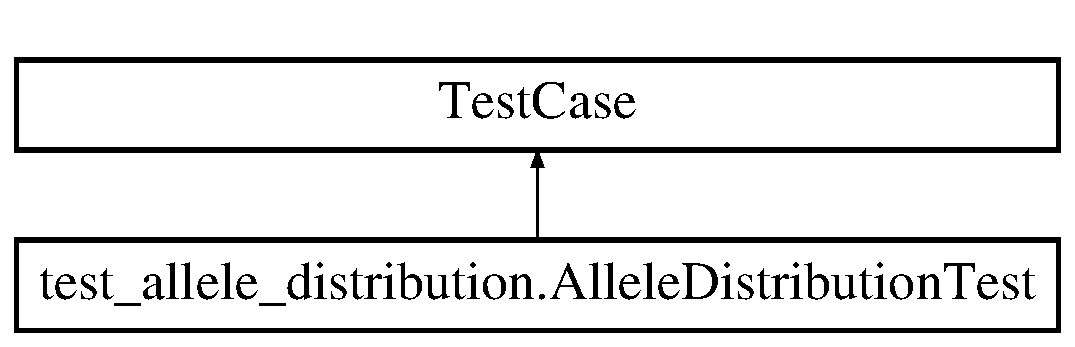
\includegraphics[height=2.000000cm]{classtest__allele__distribution_1_1_allele_distribution_test}
\end{center}
\end{figure}
\subsection*{Public Member Functions}
\begin{DoxyCompactItemize}
\item 
\hypertarget{classtest__allele__distribution_1_1_allele_distribution_test_a4381a11d850f763aa2654b6097ae79d6}{def {\bfseries test\-\_\-uniform\-\_\-10alleles}}\label{classtest__allele__distribution_1_1_allele_distribution_test_a4381a11d850f763aa2654b6097ae79d6}

\item 
\hypertarget{classtest__allele__distribution_1_1_allele_distribution_test_a12922560389617f45be6481745bcf5c5}{def {\bfseries test\-\_\-uniform\-\_\-5alleles}}\label{classtest__allele__distribution_1_1_allele_distribution_test_a12922560389617f45be6481745bcf5c5}

\item 
\hypertarget{classtest__allele__distribution_1_1_allele_distribution_test_adda324f718f761b0320b793c6c88e3ba}{def {\bfseries test\-\_\-uniform\-\_\-3alleles}}\label{classtest__allele__distribution_1_1_allele_distribution_test_adda324f718f761b0320b793c6c88e3ba}

\end{DoxyCompactItemize}


The documentation for this class was generated from the following file\-:\begin{DoxyCompactItemize}
\item 
test/test\-\_\-allele\-\_\-distribution.\-py\end{DoxyCompactItemize}

\hypertarget{classctpy_1_1data_1_1classification__data_1_1_classification_data}{\section{ctpy.\-data.\-classification\-\_\-data.\-Classification\-Data Class Reference}
\label{classctpy_1_1data_1_1classification__data_1_1_classification_data}\index{ctpy.\-data.\-classification\-\_\-data.\-Classification\-Data@{ctpy.\-data.\-classification\-\_\-data.\-Classification\-Data}}
}


A classification is represented by a dict of dimensions, each of which points to a mode definition.  


Inheritance diagram for ctpy.\-data.\-classification\-\_\-data.\-Classification\-Data\-:\begin{figure}[H]
\begin{center}
\leavevmode
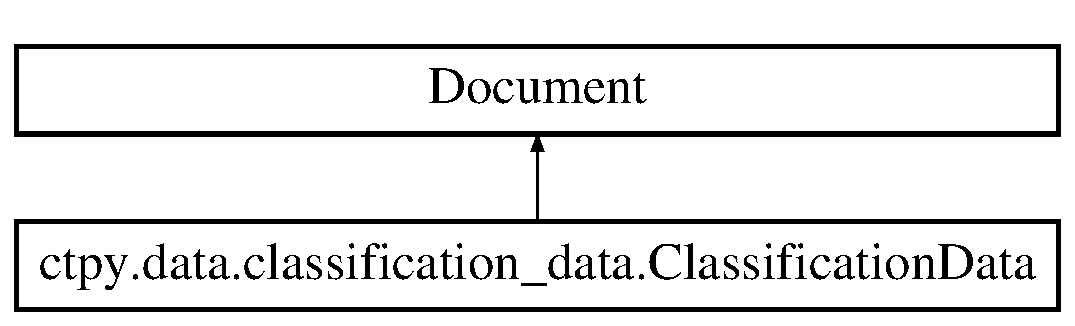
\includegraphics[height=2.000000cm]{classctpy_1_1data_1_1classification__data_1_1_classification_data}
\end{center}
\end{figure}
\subsection*{Classes}
\begin{DoxyCompactItemize}
\item 
class \hyperlink{classctpy_1_1data_1_1classification__data_1_1_classification_data_1_1____mongometa____}{\-\_\-\-\_\-mongometa\-\_\-\-\_\-}
\end{DoxyCompactItemize}
\subsection*{Static Public Attributes}
\begin{DoxyCompactItemize}
\item 
\hypertarget{classctpy_1_1data_1_1classification__data_1_1_classification_data_a0faebdc46a56568dce1bfdd7dbff188b}{tuple {\bfseries classification\-\_\-type} = Field(str)}\label{classctpy_1_1data_1_1classification__data_1_1_classification_data_a0faebdc46a56568dce1bfdd7dbff188b}

\item 
\hypertarget{classctpy_1_1data_1_1classification__data_1_1_classification_data_aad96024b8c65db43ed3618d2c01635b1}{tuple {\bfseries maxalleles} = Field(int)}\label{classctpy_1_1data_1_1classification__data_1_1_classification_data_aad96024b8c65db43ed3618d2c01635b1}

\item 
\hypertarget{classctpy_1_1data_1_1classification__data_1_1_classification_data_a07d5db6b6a8228083bc1ee38eb1de9fc}{tuple {\bfseries dimensions} = Field(int)}\label{classctpy_1_1data_1_1classification__data_1_1_classification_data_a07d5db6b6a8228083bc1ee38eb1de9fc}

\item 
\hypertarget{classctpy_1_1data_1_1classification__data_1_1_classification_data_a336bd7d4b008d108b8c08a7f6ce1cb0d}{tuple {\bfseries mean\-\_\-coarseness} = Field(float)}\label{classctpy_1_1data_1_1classification__data_1_1_classification_data_a336bd7d4b008d108b8c08a7f6ce1cb0d}

\item 
\hypertarget{classctpy_1_1data_1_1classification__data_1_1_classification_data_a5ddfc6b558a9ccd262f795cbed1a6bdb}{tuple {\bfseries modes\-\_\-for\-\_\-dimensions} = Field(\mbox{[}schema.\-Object\-Id\mbox{]})}\label{classctpy_1_1data_1_1classification__data_1_1_classification_data_a5ddfc6b558a9ccd262f795cbed1a6bdb}

\end{DoxyCompactItemize}


\subsection{Detailed Description}
A classification is represented by a dict of dimensions, each of which points to a mode definition. 



The documentation for this class was generated from the following file\-:\begin{DoxyCompactItemize}
\item 
ctpy/data/classification\-\_\-data.\-py\end{DoxyCompactItemize}

\hypertarget{classctpy_1_1data_1_1classification__mode__definitions_1_1_classification_mode_definitions}{\section{ctpy.\-data.\-classification\-\_\-mode\-\_\-definitions.\-Classification\-Mode\-Definitions Class Reference}
\label{classctpy_1_1data_1_1classification__mode__definitions_1_1_classification_mode_definitions}\index{ctpy.\-data.\-classification\-\_\-mode\-\_\-definitions.\-Classification\-Mode\-Definitions@{ctpy.\-data.\-classification\-\_\-mode\-\_\-definitions.\-Classification\-Mode\-Definitions}}
}


A classification dimension is defined by a set of modes which partition the space of the dimension.  


Inheritance diagram for ctpy.\-data.\-classification\-\_\-mode\-\_\-definitions.\-Classification\-Mode\-Definitions\-:\begin{figure}[H]
\begin{center}
\leavevmode
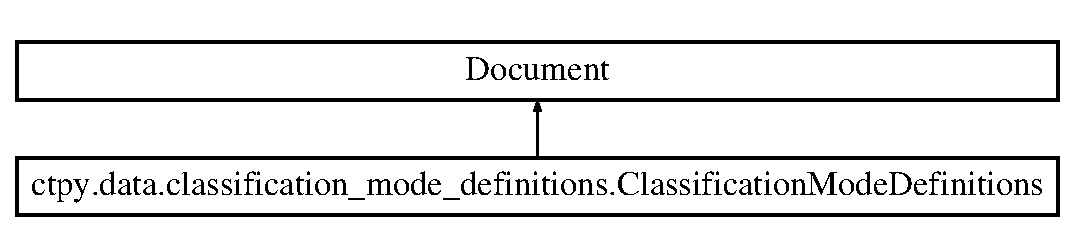
\includegraphics[height=2.000000cm]{classctpy_1_1data_1_1classification__mode__definitions_1_1_classification_mode_definitions}
\end{center}
\end{figure}
\subsection*{Classes}
\begin{DoxyCompactItemize}
\item 
class \hyperlink{classctpy_1_1data_1_1classification__mode__definitions_1_1_classification_mode_definitions_1_1____mongometa____}{\-\_\-\-\_\-mongometa\-\_\-\-\_\-}
\end{DoxyCompactItemize}


\subsection{Detailed Description}
A classification dimension is defined by a set of modes which partition the space of the dimension. 

The documentation for this class was generated from the following file\-:\begin{DoxyCompactItemize}
\item 
ctpy/data/classification\-\_\-mode\-\_\-definitions.\-py\end{DoxyCompactItemize}

\hypertarget{classctpy_1_1coarsegraining_1_1classification_1_1_classification_stats_per_sample}{\section{ctpy.\-coarsegraining.\-classification.\-Classification\-Stats\-Per\-Sample Class Reference}
\label{classctpy_1_1coarsegraining_1_1classification_1_1_classification_stats_per_sample}\index{ctpy.\-coarsegraining.\-classification.\-Classification\-Stats\-Per\-Sample@{ctpy.\-coarsegraining.\-classification.\-Classification\-Stats\-Per\-Sample}}
}
\subsection*{Public Member Functions}
\begin{DoxyCompactItemize}
\item 
\hypertarget{classctpy_1_1coarsegraining_1_1classification_1_1_classification_stats_per_sample_a3dc6686da12386c7ca84d767e2d74397}{def {\bfseries \-\_\-\-\_\-init\-\_\-\-\_\-}}\label{classctpy_1_1coarsegraining_1_1classification_1_1_classification_stats_per_sample_a3dc6686da12386c7ca84d767e2d74397}

\item 
def \hyperlink{classctpy_1_1coarsegraining_1_1classification_1_1_classification_stats_per_sample_a8873877c1648b605c1c53d159beb775b}{identify\-\_\-individual\-\_\-samples}
\begin{DoxyCompactList}\small\item\em Identify the individuals sampled from each generation of a simulation run to the appropriate class from the focal classification. \end{DoxyCompactList}\end{DoxyCompactItemize}
\subsection*{Public Attributes}
\begin{DoxyCompactItemize}
\item 
\hypertarget{classctpy_1_1coarsegraining_1_1classification_1_1_classification_stats_per_sample_a1f15c70ddc00b8d3c4dbb9f02bbe2012}{{\bfseries simconfig}}\label{classctpy_1_1coarsegraining_1_1classification_1_1_classification_stats_per_sample_a1f15c70ddc00b8d3c4dbb9f02bbe2012}

\item 
\hypertarget{classctpy_1_1coarsegraining_1_1classification_1_1_classification_stats_per_sample_a30efb7bbd6932a862b11ff7c9e44e847}{{\bfseries classification}}\label{classctpy_1_1coarsegraining_1_1classification_1_1_classification_stats_per_sample_a30efb7bbd6932a862b11ff7c9e44e847}

\item 
\hypertarget{classctpy_1_1coarsegraining_1_1classification_1_1_classification_stats_per_sample_aec04213135dd7098bff5a77ba12f3c61}{{\bfseries class\-\_\-id}}\label{classctpy_1_1coarsegraining_1_1classification_1_1_classification_stats_per_sample_aec04213135dd7098bff5a77ba12f3c61}

\item 
\hypertarget{classctpy_1_1coarsegraining_1_1classification_1_1_classification_stats_per_sample_a41eb764dcf920c2f1ead5babd5a4fd62}{{\bfseries dimensionality}}\label{classctpy_1_1coarsegraining_1_1classification_1_1_classification_stats_per_sample_a41eb764dcf920c2f1ead5babd5a4fd62}

\item 
\hypertarget{classctpy_1_1coarsegraining_1_1classification_1_1_classification_stats_per_sample_a80ce53e21e1abcd96005629de2d8325b}{{\bfseries coarseness}}\label{classctpy_1_1coarsegraining_1_1classification_1_1_classification_stats_per_sample_a80ce53e21e1abcd96005629de2d8325b}

\item 
\hypertarget{classctpy_1_1coarsegraining_1_1classification_1_1_classification_stats_per_sample_ab67521172a03bd20fdc9b3df84373515}{{\bfseries class\-\_\-type}}\label{classctpy_1_1coarsegraining_1_1classification_1_1_classification_stats_per_sample_ab67521172a03bd20fdc9b3df84373515}

\item 
\hypertarget{classctpy_1_1coarsegraining_1_1classification_1_1_classification_stats_per_sample_aeffe32767caab3a4f44dfeca524f4255}{{\bfseries save\-\_\-indiv}}\label{classctpy_1_1coarsegraining_1_1classification_1_1_classification_stats_per_sample_aeffe32767caab3a4f44dfeca524f4255}

\item 
\hypertarget{classctpy_1_1coarsegraining_1_1classification_1_1_classification_stats_per_sample_a517b549fb25f4724123dd8a5d8d989cd}{{\bfseries classification\-\_\-size}}\label{classctpy_1_1coarsegraining_1_1classification_1_1_classification_stats_per_sample_a517b549fb25f4724123dd8a5d8d989cd}

\end{DoxyCompactItemize}
\subsection*{Static Public Attributes}
\begin{DoxyCompactItemize}
\item 
\hypertarget{classctpy_1_1coarsegraining_1_1classification_1_1_classification_stats_per_sample_a4f5abbe4ff5780bde87a625a8663fc39}{tuple {\bfseries mode\-\_\-definition\-\_\-cache} = dict()}\label{classctpy_1_1coarsegraining_1_1classification_1_1_classification_stats_per_sample_a4f5abbe4ff5780bde87a625a8663fc39}

\item 
\hypertarget{classctpy_1_1coarsegraining_1_1classification_1_1_classification_stats_per_sample_a36513e0a82af30a180b9f45e19ab0a9f}{tuple {\bfseries classification\-\_\-dimension\-\_\-cache} = dict()}\label{classctpy_1_1coarsegraining_1_1classification_1_1_classification_stats_per_sample_a36513e0a82af30a180b9f45e19ab0a9f}

\end{DoxyCompactItemize}


\subsection{Member Function Documentation}
\hypertarget{classctpy_1_1coarsegraining_1_1classification_1_1_classification_stats_per_sample_a8873877c1648b605c1c53d159beb775b}{\index{ctpy\-::coarsegraining\-::classification\-::\-Classification\-Stats\-Per\-Sample@{ctpy\-::coarsegraining\-::classification\-::\-Classification\-Stats\-Per\-Sample}!identify\-\_\-individual\-\_\-samples@{identify\-\_\-individual\-\_\-samples}}
\index{identify\-\_\-individual\-\_\-samples@{identify\-\_\-individual\-\_\-samples}!ctpy::coarsegraining::classification::ClassificationStatsPerSample@{ctpy\-::coarsegraining\-::classification\-::\-Classification\-Stats\-Per\-Sample}}
\subsubsection[{identify\-\_\-individual\-\_\-samples}]{\setlength{\rightskip}{0pt plus 5cm}def ctpy.\-coarsegraining.\-classification.\-Classification\-Stats\-Per\-Sample.\-identify\-\_\-individual\-\_\-samples (
\begin{DoxyParamCaption}
\item[{}]{self}
\end{DoxyParamCaption}
)}}\label{classctpy_1_1coarsegraining_1_1classification_1_1_classification_stats_per_sample_a8873877c1648b605c1c53d159beb775b}


Identify the individuals sampled from each generation of a simulation run to the appropriate class from the focal classification. 

Each \char`\"{}sample\char`\"{} is a record from one generation of one replication of one simulation run, at a given sample size and dimensionality. Within each sample record is a list of sampled individual genotypes. This list is what we iterate over to identify via the classification, and then we calculate various stats, and store the resulting stats. If the flag for saving raw individuals (after classification identification) is set, we also store the list of individuals and the classes to which their genotypes identify.

\-:return\-: None 

The documentation for this class was generated from the following file\-:\begin{DoxyCompactItemize}
\item 
ctpy/coarsegraining/classification.\-py\end{DoxyCompactItemize}

\hypertarget{classctpy_1_1coarsegraining_1_1classification_1_1_classification_stats_per_simrun}{\section{ctpy.\-coarsegraining.\-classification.\-Classification\-Stats\-Per\-Simrun Class Reference}
\label{classctpy_1_1coarsegraining_1_1classification_1_1_classification_stats_per_simrun}\index{ctpy.\-coarsegraining.\-classification.\-Classification\-Stats\-Per\-Simrun@{ctpy.\-coarsegraining.\-classification.\-Classification\-Stats\-Per\-Simrun}}
}
\subsection*{Public Member Functions}
\begin{DoxyCompactItemize}
\item 
\hypertarget{classctpy_1_1coarsegraining_1_1classification_1_1_classification_stats_per_simrun_ab5221d9eb26315dc3e912d6cd85ae9fb}{def {\bfseries \-\_\-\-\_\-init\-\_\-\-\_\-}}\label{classctpy_1_1coarsegraining_1_1classification_1_1_classification_stats_per_simrun_ab5221d9eb26315dc3e912d6cd85ae9fb}

\item 
def \hyperlink{classctpy_1_1coarsegraining_1_1classification_1_1_classification_stats_per_simrun_a92bf4508aa14b53c4e1b13a0dd96dccb}{process\-\_\-simulation\-\_\-run}
\begin{DoxyCompactList}\small\item\em Process the individual samples for a single simulation run, calculating any statistics that require aggregation over the simulation run, saving the results to the database. \end{DoxyCompactList}\end{DoxyCompactItemize}
\subsection*{Public Attributes}
\begin{DoxyCompactItemize}
\item 
\hypertarget{classctpy_1_1coarsegraining_1_1classification_1_1_classification_stats_per_simrun_a4434a9162d24c6335a9aaf1240d8a6b7}{{\bfseries simconfig}}\label{classctpy_1_1coarsegraining_1_1classification_1_1_classification_stats_per_simrun_a4434a9162d24c6335a9aaf1240d8a6b7}

\item 
\hypertarget{classctpy_1_1coarsegraining_1_1classification_1_1_classification_stats_per_simrun_a1a042e351fb73ec03e5ac175dcf14389}{{\bfseries simrun\-\_\-param\-\_\-cache}}\label{classctpy_1_1coarsegraining_1_1classification_1_1_classification_stats_per_simrun_a1a042e351fb73ec03e5ac175dcf14389}

\item 
\hypertarget{classctpy_1_1coarsegraining_1_1classification_1_1_classification_stats_per_simrun_aeca79e2cd17c19e06c97cbd8fff83788}{{\bfseries param\-\_\-cached}}\label{classctpy_1_1coarsegraining_1_1classification_1_1_classification_stats_per_simrun_aeca79e2cd17c19e06c97cbd8fff83788}

\end{DoxyCompactItemize}


\subsection{Member Function Documentation}
\hypertarget{classctpy_1_1coarsegraining_1_1classification_1_1_classification_stats_per_simrun_a92bf4508aa14b53c4e1b13a0dd96dccb}{\index{ctpy\-::coarsegraining\-::classification\-::\-Classification\-Stats\-Per\-Simrun@{ctpy\-::coarsegraining\-::classification\-::\-Classification\-Stats\-Per\-Simrun}!process\-\_\-simulation\-\_\-run@{process\-\_\-simulation\-\_\-run}}
\index{process\-\_\-simulation\-\_\-run@{process\-\_\-simulation\-\_\-run}!ctpy::coarsegraining::classification::ClassificationStatsPerSimrun@{ctpy\-::coarsegraining\-::classification\-::\-Classification\-Stats\-Per\-Simrun}}
\subsubsection[{process\-\_\-simulation\-\_\-run}]{\setlength{\rightskip}{0pt plus 5cm}def ctpy.\-coarsegraining.\-classification.\-Classification\-Stats\-Per\-Simrun.\-process\-\_\-simulation\-\_\-run (
\begin{DoxyParamCaption}
\item[{}]{self, }
\item[{}]{simrun\-\_\-id}
\end{DoxyParamCaption}
)}}\label{classctpy_1_1coarsegraining_1_1classification_1_1_classification_stats_per_simrun_a92bf4508aa14b53c4e1b13a0dd96dccb}


Process the individual samples for a single simulation run, calculating any statistics that require aggregation over the simulation run, saving the results to the database. 

This requires that we process each \char`\"{}replication\char`\"{} separately, so that we do not mix them together.

\-:return\-: 

The documentation for this class was generated from the following file\-:\begin{DoxyCompactItemize}
\item 
ctpy/coarsegraining/classification.\-py\end{DoxyCompactItemize}

\hypertarget{classtest__configuration_1_1_configuration_test}{\section{test\-\_\-configuration.\-Configuration\-Test Class Reference}
\label{classtest__configuration_1_1_configuration_test}\index{test\-\_\-configuration.\-Configuration\-Test@{test\-\_\-configuration.\-Configuration\-Test}}
}
Inheritance diagram for test\-\_\-configuration.\-Configuration\-Test\-:\begin{figure}[H]
\begin{center}
\leavevmode
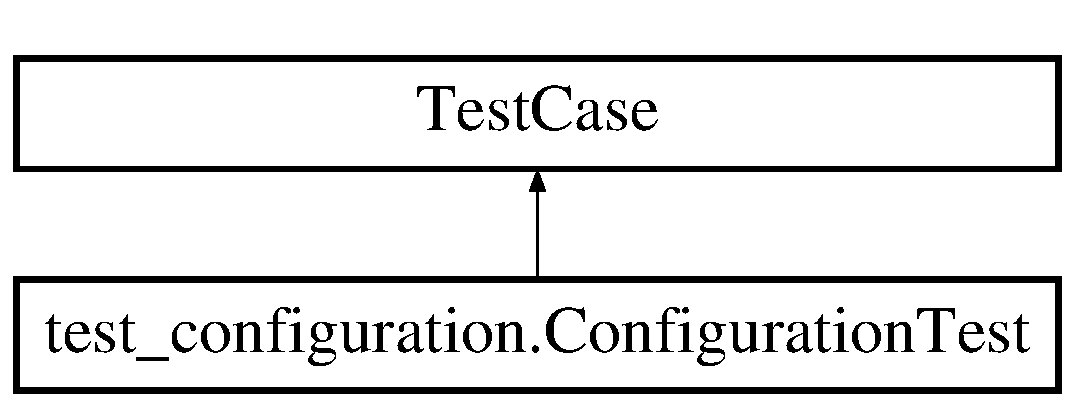
\includegraphics[height=2.000000cm]{classtest__configuration_1_1_configuration_test}
\end{center}
\end{figure}
\subsection*{Public Member Functions}
\begin{DoxyCompactItemize}
\item 
\hypertarget{classtest__configuration_1_1_configuration_test_ad469b92cd21087bdce65770727628c58}{def {\bfseries set\-Up}}\label{classtest__configuration_1_1_configuration_test_ad469b92cd21087bdce65770727628c58}

\item 
\hypertarget{classtest__configuration_1_1_configuration_test_aff4b1244aa951499069307cc282401e2}{def {\bfseries tear\-Down}}\label{classtest__configuration_1_1_configuration_test_aff4b1244aa951499069307cc282401e2}

\item 
\hypertarget{classtest__configuration_1_1_configuration_test_a3a77773b5cb19ef4a090c77ed9017fd6}{def {\bfseries test\-\_\-configuration}}\label{classtest__configuration_1_1_configuration_test_a3a77773b5cb19ef4a090c77ed9017fd6}

\item 
\hypertarget{classtest__configuration_1_1_configuration_test_a7b47ad52641e965723f4d68cffa1bd12}{def {\bfseries test\-\_\-latex\-\_\-output}}\label{classtest__configuration_1_1_configuration_test_a7b47ad52641e965723f4d68cffa1bd12}

\item 
\hypertarget{classtest__configuration_1_1_configuration_test_ab2abe2b5082506f29f1d2dd3ae2e636b}{def {\bfseries test\-\_\-pandoc\-\_\-output}}\label{classtest__configuration_1_1_configuration_test_ab2abe2b5082506f29f1d2dd3ae2e636b}

\end{DoxyCompactItemize}
\subsection*{Public Attributes}
\begin{DoxyCompactItemize}
\item 
\hypertarget{classtest__configuration_1_1_configuration_test_a17b43808c59024e2240c485331e2ec1f}{{\bfseries tf}}\label{classtest__configuration_1_1_configuration_test_a17b43808c59024e2240c485331e2ec1f}

\end{DoxyCompactItemize}
\subsection*{Static Public Attributes}
\begin{DoxyCompactItemize}
\item 
\hypertarget{classtest__configuration_1_1_configuration_test_a73ef01cf9f31d245934eadf2c4279d89}{string {\bfseries filename} = \char`\"{}test\char`\"{}}\label{classtest__configuration_1_1_configuration_test_a73ef01cf9f31d245934eadf2c4279d89}

\end{DoxyCompactItemize}


The documentation for this class was generated from the following file\-:\begin{DoxyCompactItemize}
\item 
test/test\-\_\-configuration.\-py\end{DoxyCompactItemize}

\hypertarget{classctpy_1_1strategies_1_1conformism_1_1_conformist_mating_scheme}{\section{ctpy.\-strategies.\-conformism.\-Conformist\-Mating\-Scheme Class Reference}
\label{classctpy_1_1strategies_1_1conformism_1_1_conformist_mating_scheme}\index{ctpy.\-strategies.\-conformism.\-Conformist\-Mating\-Scheme@{ctpy.\-strategies.\-conformism.\-Conformist\-Mating\-Scheme}}
}


A homogeneous mating scheme which implements a variety of \char`\"{}conformist\char`\"{} transmission rules.  


Inheritance diagram for ctpy.\-strategies.\-conformism.\-Conformist\-Mating\-Scheme\-:\begin{figure}[H]
\begin{center}
\leavevmode
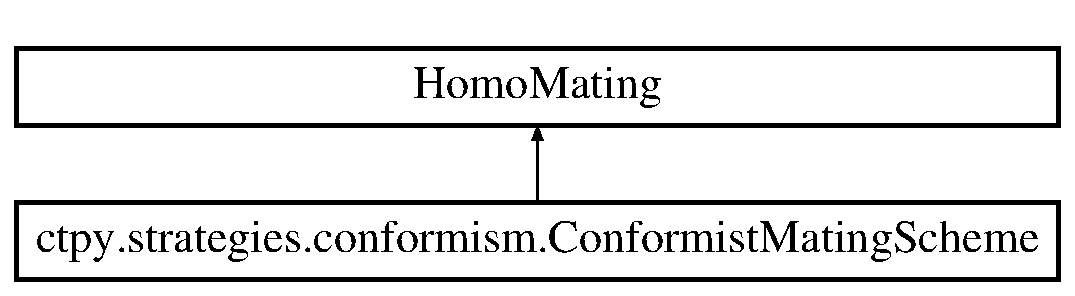
\includegraphics[height=2.000000cm]{classctpy_1_1strategies_1_1conformism_1_1_conformist_mating_scheme}
\end{center}
\end{figure}
\subsection*{Public Member Functions}
\begin{DoxyCompactItemize}
\item 
\hypertarget{classctpy_1_1strategies_1_1conformism_1_1_conformist_mating_scheme_abb9cbd891f0d3a9aeaa215667545d33f}{def {\bfseries \-\_\-\-\_\-init\-\_\-\-\_\-}}\label{classctpy_1_1strategies_1_1conformism_1_1_conformist_mating_scheme_abb9cbd891f0d3a9aeaa215667545d33f}

\item 
\hypertarget{classctpy_1_1strategies_1_1conformism_1_1_conformist_mating_scheme_a45b0ad3f6028fed92b50dcd45ac6533e}{def \hyperlink{classctpy_1_1strategies_1_1conformism_1_1_conformist_mating_scheme_a45b0ad3f6028fed92b50dcd45ac6533e}{prob\-Select\-Parent\-With\-Most\-Popular\-Traits}}\label{classctpy_1_1strategies_1_1conformism_1_1_conformist_mating_scheme_a45b0ad3f6028fed92b50dcd45ac6533e}

\begin{DoxyCompactList}\small\item\em Selects parents with the \char`\"{}most popular\char`\"{} traits, with probability. \end{DoxyCompactList}\end{DoxyCompactItemize}


\subsection{Detailed Description}
A homogeneous mating scheme which implements a variety of \char`\"{}conformist\char`\"{} transmission rules. 

The documentation for this class was generated from the following file\-:\begin{DoxyCompactItemize}
\item 
ctpy/strategies/conformism.\-py\end{DoxyCompactItemize}

\hypertarget{classctpy_1_1utils_1_1configuration_1_1_c_t_py_configuration}{\section{ctpy.\-utils.\-configuration.\-C\-T\-Py\-Configuration Class Reference}
\label{classctpy_1_1utils_1_1configuration_1_1_c_t_py_configuration}\index{ctpy.\-utils.\-configuration.\-C\-T\-Py\-Configuration@{ctpy.\-utils.\-configuration.\-C\-T\-Py\-Configuration}}
}
\subsection*{Public Member Functions}
\begin{DoxyCompactItemize}
\item 
\hypertarget{classctpy_1_1utils_1_1configuration_1_1_c_t_py_configuration_adbb9201a49e6b4c5feaaf1cb31a5eb3b}{def {\bfseries \-\_\-\-\_\-init\-\_\-\-\_\-}}\label{classctpy_1_1utils_1_1configuration_1_1_c_t_py_configuration_adbb9201a49e6b4c5feaaf1cb31a5eb3b}

\item 
\hypertarget{classctpy_1_1utils_1_1configuration_1_1_c_t_py_configuration_af70073aca0f56ad01a38c56a712c4ece}{def {\bfseries \-\_\-\-\_\-repr\-\_\-\-\_\-}}\label{classctpy_1_1utils_1_1configuration_1_1_c_t_py_configuration_af70073aca0f56ad01a38c56a712c4ece}

\item 
def \hyperlink{classctpy_1_1utils_1_1configuration_1_1_c_t_py_configuration_abed8bebe92b3bc48b3ed87c64e102f35}{to\-\_\-latex\-\_\-table}
\begin{DoxyCompactList}\small\item\em Constructs a La\-Te\-X table and tabular environment for the simulation parameters and control variable settings. \end{DoxyCompactList}\item 
def \hyperlink{classctpy_1_1utils_1_1configuration_1_1_c_t_py_configuration_a3693c03da84920bc9f8a0d77f4e7f976}{to\-\_\-pandoc\-\_\-table}
\begin{DoxyCompactList}\small\item\em Constructs a Markdown table (in pandoc format) for the simulation parameters and control variable settings. \end{DoxyCompactList}\end{DoxyCompactItemize}
\subsection*{Public Attributes}
\begin{DoxyCompactItemize}
\item 
\hypertarget{classctpy_1_1utils_1_1configuration_1_1_c_t_py_configuration_a54210799908da15bc8320ace48528e23}{{\bfseries config}}\label{classctpy_1_1utils_1_1configuration_1_1_c_t_py_configuration_a54210799908da15bc8320ace48528e23}

\item 
\hypertarget{classctpy_1_1utils_1_1configuration_1_1_c_t_py_configuration_a052fd16ce5b0ada7df66e4f05261b52d}{{\bfseries N\-U\-M\-\_\-\-S\-A\-M\-P\-L\-E\-S\-\_\-\-A\-N\-A\-L\-Y\-Z\-E\-D\-\_\-\-P\-E\-R\-\_\-\-F\-I\-N\-A\-L\-\_\-\-S\-A\-M\-P\-L\-E\-\_\-\-P\-A\-T\-H}}\label{classctpy_1_1utils_1_1configuration_1_1_c_t_py_configuration_a052fd16ce5b0ada7df66e4f05261b52d}

\end{DoxyCompactItemize}
\subsection*{Static Public Attributes}
\begin{DoxyCompactItemize}
\item 
\hypertarget{classctpy_1_1utils_1_1configuration_1_1_c_t_py_configuration_aa813fec1e5c80d6e14b66f45c80f1b60}{tuple {\bfseries M\-O\-D\-E\-T\-Y\-P\-E\-\_\-\-E\-V\-E\-N} = str(\char`\"{}E\-V\-E\-N\char`\"{})}\label{classctpy_1_1utils_1_1configuration_1_1_c_t_py_configuration_aa813fec1e5c80d6e14b66f45c80f1b60}

\item 
\hypertarget{classctpy_1_1utils_1_1configuration_1_1_c_t_py_configuration_aa071918fa157efea06a7b19f8032d6e4}{tuple {\bfseries M\-O\-D\-E\-T\-Y\-P\-E\-\_\-\-R\-A\-N\-D\-O\-M} = str('R\-A\-N\-D\-O\-M')}\label{classctpy_1_1utils_1_1configuration_1_1_c_t_py_configuration_aa071918fa157efea06a7b19f8032d6e4}

\item 
\hypertarget{classctpy_1_1utils_1_1configuration_1_1_c_t_py_configuration_a07120c4edf79fb3d8dd463f94673ba48}{int {\bfseries S\-L\-A\-T\-K\-I\-N\-\_\-\-M\-O\-N\-T\-E\-C\-A\-R\-L\-O\-\_\-\-R\-E\-P\-L\-I\-C\-A\-T\-E\-S} = 10000}\label{classctpy_1_1utils_1_1configuration_1_1_c_t_py_configuration_a07120c4edf79fb3d8dd463f94673ba48}

\item 
\hypertarget{classctpy_1_1utils_1_1configuration_1_1_c_t_py_configuration_ae612fd6b9bfbead69156fc7d28d15a38}{int \hyperlink{classctpy_1_1utils_1_1configuration_1_1_c_t_py_configuration_ae612fd6b9bfbead69156fc7d28d15a38}{M\-A\-X\-A\-L\-L\-E\-L\-E\-S} = 1000000000}\label{classctpy_1_1utils_1_1configuration_1_1_c_t_py_configuration_ae612fd6b9bfbead69156fc7d28d15a38}

\begin{DoxyCompactList}\small\item\em Research-\/level constants. \end{DoxyCompactList}\item 
\hypertarget{classctpy_1_1utils_1_1configuration_1_1_c_t_py_configuration_ab30a00cf60918969bf12fd0a4e7369a0}{int {\bfseries N\-U\-M\-\_\-\-R\-E\-P\-L\-I\-C\-A\-T\-E\-S\-\_\-\-F\-O\-R\-\_\-\-R\-A\-N\-D\-O\-M\-\_\-\-D\-I\-M\-E\-N\-S\-I\-O\-N\-\_\-\-M\-O\-D\-E\-S} = 10}\label{classctpy_1_1utils_1_1configuration_1_1_c_t_py_configuration_ab30a00cf60918969bf12fd0a4e7369a0}

\item 
\hypertarget{classctpy_1_1utils_1_1configuration_1_1_c_t_py_configuration_a89842ee405e327fa3693ed6c18a76528}{list {\bfseries D\-I\-M\-E\-N\-S\-I\-O\-N\-\_\-\-P\-A\-R\-T\-I\-T\-I\-O\-N\-S} = \mbox{[}2,3,4,8,16,32\mbox{]}}\label{classctpy_1_1utils_1_1configuration_1_1_c_t_py_configuration_a89842ee405e327fa3693ed6c18a76528}

\item 
\hypertarget{classctpy_1_1utils_1_1configuration_1_1_c_t_py_configuration_acfc622926aabf1367f72065dc69232ea}{list {\bfseries D\-I\-M\-E\-N\-S\-I\-O\-N\-S\-\_\-\-S\-T\-U\-D\-I\-E\-D} = \mbox{[}2,3,4,6,8\mbox{]}}\label{classctpy_1_1utils_1_1configuration_1_1_c_t_py_configuration_acfc622926aabf1367f72065dc69232ea}

\item 
\hypertarget{classctpy_1_1utils_1_1configuration_1_1_c_t_py_configuration_a09901731aea99c438ed336557fdc2708}{list {\bfseries I\-N\-N\-O\-V\-A\-T\-I\-O\-N\-\_\-\-R\-A\-T\-E\-S\-\_\-\-S\-T\-U\-D\-I\-E\-D} = \mbox{[}0.\-0001,0.\-00025,0.\-0005,0.\-001,0.\-0025,0.\-005,0.\-01,0.\-025\mbox{]}}\label{classctpy_1_1utils_1_1configuration_1_1_c_t_py_configuration_a09901731aea99c438ed336557fdc2708}

\item 
\hypertarget{classctpy_1_1utils_1_1configuration_1_1_c_t_py_configuration_a28bbeedd6c10b248b1d3615138a88be3}{int {\bfseries S\-I\-M\-U\-L\-A\-T\-I\-O\-N\-\_\-\-L\-E\-N\-G\-T\-H\-\_\-\-A\-F\-T\-E\-R\-\_\-\-S\-T\-A\-T\-I\-O\-N\-A\-R\-I\-T\-Y} = 10000}\label{classctpy_1_1utils_1_1configuration_1_1_c_t_py_configuration_a28bbeedd6c10b248b1d3615138a88be3}

\item 
\hypertarget{classctpy_1_1utils_1_1configuration_1_1_c_t_py_configuration_aae958167a9ac940a31ebd14c4cfa58c2}{list {\bfseries T\-I\-M\-E\-\_\-\-A\-V\-E\-R\-A\-G\-I\-N\-G\-\_\-\-D\-U\-R\-A\-T\-I\-O\-N\-S\-\_\-\-S\-T\-U\-D\-I\-E\-D} = \mbox{[}1000,500,250,125,63,32,16,8,1\mbox{]}}\label{classctpy_1_1utils_1_1configuration_1_1_c_t_py_configuration_aae958167a9ac940a31ebd14c4cfa58c2}

\item 
\hypertarget{classctpy_1_1utils_1_1configuration_1_1_c_t_py_configuration_ac00ba87d08ec209c61c93a8169525410}{int {\bfseries I\-N\-I\-T\-I\-A\-L\-\_\-\-T\-R\-A\-I\-T\-\_\-\-N\-U\-M\-B\-E\-R} = 10}\label{classctpy_1_1utils_1_1configuration_1_1_c_t_py_configuration_ac00ba87d08ec209c61c93a8169525410}

\item 
\hypertarget{classctpy_1_1utils_1_1configuration_1_1_c_t_py_configuration_aae400a6af08ceb075da1ba90abb2fed4}{int {\bfseries S\-A\-M\-P\-L\-I\-N\-G\-\_\-\-I\-N\-T\-E\-R\-V\-A\-L} = 1}\label{classctpy_1_1utils_1_1configuration_1_1_c_t_py_configuration_aae400a6af08ceb075da1ba90abb2fed4}

\item 
\hypertarget{classctpy_1_1utils_1_1configuration_1_1_c_t_py_configuration_a1bbcbf5c6b2e29647b64c693122fcb0b}{int {\bfseries R\-E\-P\-L\-I\-C\-A\-T\-I\-O\-N\-S\-\_\-\-P\-E\-R\-\_\-\-P\-A\-R\-A\-M\-\_\-\-S\-E\-T} = 10}\label{classctpy_1_1utils_1_1configuration_1_1_c_t_py_configuration_a1bbcbf5c6b2e29647b64c693122fcb0b}

\item 
\hypertarget{classctpy_1_1utils_1_1configuration_1_1_c_t_py_configuration_aaac008492674f70791c1176e39746b7c}{list {\bfseries S\-A\-M\-P\-L\-E\-\_\-\-S\-I\-Z\-E\-S\-\_\-\-S\-T\-U\-D\-I\-E\-D} = \mbox{[}25,50,100,200\mbox{]}}\label{classctpy_1_1utils_1_1configuration_1_1_c_t_py_configuration_aaac008492674f70791c1176e39746b7c}

\item 
\hypertarget{classctpy_1_1utils_1_1configuration_1_1_c_t_py_configuration_a1dafedca7d79e57ba40c9c576143900e}{list {\bfseries P\-O\-P\-U\-L\-A\-T\-I\-O\-N\-\_\-\-S\-I\-Z\-E\-S\-\_\-\-S\-T\-U\-D\-I\-E\-D} = \mbox{[}500,1000,2500,5000\mbox{]}}\label{classctpy_1_1utils_1_1configuration_1_1_c_t_py_configuration_a1dafedca7d79e57ba40c9c576143900e}

\item 
\hypertarget{classctpy_1_1utils_1_1configuration_1_1_c_t_py_configuration_a32fdaa7016b928746886eb1171042ea5}{list {\bfseries D\-E\-M\-E\-\_\-\-N\-U\-M\-B\-E\-R\-S\-\_\-\-S\-T\-U\-D\-I\-E\-D} = \mbox{[}32\mbox{]}}\label{classctpy_1_1utils_1_1configuration_1_1_c_t_py_configuration_a32fdaa7016b928746886eb1171042ea5}

\item 
\hypertarget{classctpy_1_1utils_1_1configuration_1_1_c_t_py_configuration_ab3f4b06e4d980c7213fe2cdf9af4ee21}{int {\bfseries N\-U\-M\-B\-E\-R\-\_\-\-R\-A\-N\-D\-O\-M\-\_\-\-M\-I\-G\-R\-A\-T\-I\-O\-N\-\_\-\-M\-A\-T\-R\-I\-C\-E\-S\-\_\-\-S\-T\-U\-D\-I\-E\-D} = 10}\label{classctpy_1_1utils_1_1configuration_1_1_c_t_py_configuration_ab3f4b06e4d980c7213fe2cdf9af4ee21}

\item 
\hypertarget{classctpy_1_1utils_1_1configuration_1_1_c_t_py_configuration_a1732fed6532f6791470984c6aa93b5b3}{list {\bfseries D\-E\-N\-S\-I\-T\-Y\-\_\-\-S\-M\-A\-L\-L\-\_\-\-W\-O\-R\-L\-D\-\_\-\-L\-I\-N\-K\-S\-\_\-\-S\-T\-U\-D\-I\-E\-D} = \mbox{[}0.\-0,0.\-1,0.\-25,0.\-5,0.\-75\mbox{]}}\label{classctpy_1_1utils_1_1configuration_1_1_c_t_py_configuration_a1732fed6532f6791470984c6aa93b5b3}

\item 
\hypertarget{classctpy_1_1utils_1_1configuration_1_1_c_t_py_configuration_a447666e9624d05209a6f0895b50a4225}{list {\bfseries C\-L\-U\-S\-T\-E\-R\-I\-N\-G\-\_\-\-C\-O\-E\-F\-F\-I\-C\-I\-E\-N\-T\-S\-\_\-\-S\-T\-U\-D\-I\-E\-D} = \mbox{[}0.\-0,0.\-1,0.\-25,0.\-5,0.\-75\mbox{]}}\label{classctpy_1_1utils_1_1configuration_1_1_c_t_py_configuration_a447666e9624d05209a6f0895b50a4225}

\item 
\hypertarget{classctpy_1_1utils_1_1configuration_1_1_c_t_py_configuration_a9be3bb52eeaf49da39e0cf5520c074e8}{int {\bfseries N\-U\-M\-\_\-\-S\-A\-M\-P\-L\-E\-S\-\_\-\-A\-N\-A\-L\-Y\-Z\-E\-D\-\_\-\-P\-E\-R\-\_\-\-F\-I\-N\-A\-L\-\_\-\-S\-A\-M\-P\-L\-E\-\_\-\-P\-A\-T\-H} = 1}\label{classctpy_1_1utils_1_1configuration_1_1_c_t_py_configuration_a9be3bb52eeaf49da39e0cf5520c074e8}

\item 
dictionary {\bfseries parameter\-\_\-labels}
\item 
\hypertarget{classctpy_1_1utils_1_1configuration_1_1_c_t_py_configuration_a8e8b666431ab422770c3c675a369f124}{list {\bfseries vars\-\_\-to\-\_\-filter} = \mbox{[}'config', 'T\-I\-M\-E\-\_\-\-A\-V\-E\-R\-A\-G\-I\-N\-G\-\_\-\-D\-U\-R\-A\-T\-I\-O\-N\-S\-\_\-\-S\-T\-U\-D\-I\-E\-D', 'M\-O\-D\-E\-T\-Y\-P\-E\-\_\-\-E\-V\-E\-N','M\-O\-D\-E\-T\-Y\-P\-E\-\_\-\-R\-A\-N\-D\-O\-M','\hyperlink{classctpy_1_1utils_1_1configuration_1_1_c_t_py_configuration_ae612fd6b9bfbead69156fc7d28d15a38}{M\-A\-X\-A\-L\-L\-E\-L\-E\-S}','D\-E\-M\-E\-\_\-\-N\-U\-M\-B\-E\-R\-S\-\_\-\-S\-T\-U\-D\-I\-E\-D','N\-U\-M\-B\-E\-R\-\_\-\-R\-A\-N\-D\-O\-M\-\_\-\-M\-I\-G\-R\-A\-T\-I\-O\-N\-\_\-\-M\-A\-T\-R\-I\-C\-E\-S\-\_\-\-S\-T\-U\-D\-I\-E\-D','D\-E\-N\-S\-I\-T\-Y\-\_\-\-S\-M\-A\-L\-L\-\_\-\-W\-O\-R\-L\-D\-\_\-\-L\-I\-N\-K\-S\-\_\-\-S\-T\-U\-D\-I\-E\-D','C\-L\-U\-S\-T\-E\-R\-I\-N\-G\-\_\-\-C\-O\-E\-F\-F\-I\-C\-I\-E\-N\-T\-S\-\_\-\-S\-T\-U\-D\-I\-E\-D'\mbox{]}}\label{classctpy_1_1utils_1_1configuration_1_1_c_t_py_configuration_a8e8b666431ab422770c3c675a369f124}

\end{DoxyCompactItemize}


\subsection{Member Function Documentation}
\hypertarget{classctpy_1_1utils_1_1configuration_1_1_c_t_py_configuration_abed8bebe92b3bc48b3ed87c64e102f35}{\index{ctpy\-::utils\-::configuration\-::\-C\-T\-Py\-Configuration@{ctpy\-::utils\-::configuration\-::\-C\-T\-Py\-Configuration}!to\-\_\-latex\-\_\-table@{to\-\_\-latex\-\_\-table}}
\index{to\-\_\-latex\-\_\-table@{to\-\_\-latex\-\_\-table}!ctpy::utils::configuration::CTPyConfiguration@{ctpy\-::utils\-::configuration\-::\-C\-T\-Py\-Configuration}}
\subsubsection[{to\-\_\-latex\-\_\-table}]{\setlength{\rightskip}{0pt plus 5cm}def ctpy.\-utils.\-configuration.\-C\-T\-Py\-Configuration.\-to\-\_\-latex\-\_\-table (
\begin{DoxyParamCaption}
\item[{}]{self, }
\item[{}]{experiment, }
\item[{}]{kwargs}
\end{DoxyParamCaption}
)}}\label{classctpy_1_1utils_1_1configuration_1_1_c_t_py_configuration_abed8bebe92b3bc48b3ed87c64e102f35}


Constructs a La\-Te\-X table and tabular environment for the simulation parameters and control variable settings. 

A list of \char`\"{}internal\char`\"{} or unimplemented variables are filtered out of this list, and actual variable names are translated to human-\/readable phrases with a lookup table.

Takes an optional named argument\-: caption=String. This parameter will replace the caption automatically generated by this method.

\-:return\-: A string comprising the La\-Te\-X representation for the parameters. \hypertarget{classctpy_1_1utils_1_1configuration_1_1_c_t_py_configuration_a3693c03da84920bc9f8a0d77f4e7f976}{\index{ctpy\-::utils\-::configuration\-::\-C\-T\-Py\-Configuration@{ctpy\-::utils\-::configuration\-::\-C\-T\-Py\-Configuration}!to\-\_\-pandoc\-\_\-table@{to\-\_\-pandoc\-\_\-table}}
\index{to\-\_\-pandoc\-\_\-table@{to\-\_\-pandoc\-\_\-table}!ctpy::utils::configuration::CTPyConfiguration@{ctpy\-::utils\-::configuration\-::\-C\-T\-Py\-Configuration}}
\subsubsection[{to\-\_\-pandoc\-\_\-table}]{\setlength{\rightskip}{0pt plus 5cm}def ctpy.\-utils.\-configuration.\-C\-T\-Py\-Configuration.\-to\-\_\-pandoc\-\_\-table (
\begin{DoxyParamCaption}
\item[{}]{self, }
\item[{}]{experiment, }
\item[{}]{kwargs}
\end{DoxyParamCaption}
)}}\label{classctpy_1_1utils_1_1configuration_1_1_c_t_py_configuration_a3693c03da84920bc9f8a0d77f4e7f976}


Constructs a Markdown table (in pandoc format) for the simulation parameters and control variable settings. 

A list of \char`\"{}internal\char`\"{} or unimplemented variables are filtered out of this list, and actual variable names are translated to human-\/readable phrases with a lookup table.

\-:return\-: Text string representing a Pandoc table 

\subsection{Member Data Documentation}
\hypertarget{classctpy_1_1utils_1_1configuration_1_1_c_t_py_configuration_a32b0c831d473a6aa1968f98d46415820}{\index{ctpy\-::utils\-::configuration\-::\-C\-T\-Py\-Configuration@{ctpy\-::utils\-::configuration\-::\-C\-T\-Py\-Configuration}!parameter\-\_\-labels@{parameter\-\_\-labels}}
\index{parameter\-\_\-labels@{parameter\-\_\-labels}!ctpy::utils::configuration::CTPyConfiguration@{ctpy\-::utils\-::configuration\-::\-C\-T\-Py\-Configuration}}
\subsubsection[{parameter\-\_\-labels}]{\setlength{\rightskip}{0pt plus 5cm}dictionary ctpy.\-utils.\-configuration.\-C\-T\-Py\-Configuration.\-parameter\-\_\-labels\hspace{0.3cm}{\ttfamily [static]}}}\label{classctpy_1_1utils_1_1configuration_1_1_c_t_py_configuration_a32b0c831d473a6aa1968f98d46415820}
{\bfseries Initial value\-:}
\begin{DoxyCode}
1 = \{
2         \textcolor{stringliteral}{'NUM\_SAMPLES\_ANALYZED\_PER\_FINAL\_SAMPLE\_PATH'} : \textcolor{stringliteral}{'Num samples taken after stationarity, per run'},
3         \textcolor{stringliteral}{'POPULATION\_SIZES\_STUDIED'} : \textcolor{stringliteral}{'Population sizes'},
4         \textcolor{stringliteral}{'SAMPLE\_SIZES\_STUDIED'} : \textcolor{stringliteral}{'Sample sizes taken at each sampling interval'},
5         \textcolor{stringliteral}{'REPLICATIONS\_PER\_PARAM\_SET'} : \textcolor{stringliteral}{'Replicate simulation runs at each parameter combination'},
6         \textcolor{stringliteral}{'SAMPLING\_INTERVAL'} : \textcolor{stringliteral}{'Interval in generations for samples after stationarity'},
7         \textcolor{stringliteral}{'INITIAL\_TRAIT\_NUMBER'} : \textcolor{stringliteral}{'Number of traits per dimension for initializing population'},
8         \textcolor{stringliteral}{'SIMULATION\_LENGTH\_AFTER\_STATIONARITY'} : \textcolor{stringliteral}{'Length of simulation run after stationarity'},
9         \textcolor{stringliteral}{'INNOVATION\_RATES\_STUDIED'} : \textcolor{stringliteral}{'Innovation rates (event probability per person per generation)'},
10         \textcolor{stringliteral}{'DIMENSIONS\_STUDIED'} : \textcolor{stringliteral}{'Trait and classification dimensionalities'},
11         \textcolor{stringliteral}{'DIMENSION\_PARTITIONS'} : \textcolor{stringliteral}{'Classification coarseness levels (modes per dimension)'},
12         \textcolor{stringliteral}{'NUM\_REPLICATES\_FOR\_RANDOM\_DIMENSION\_MODES'} : \textcolor{stringliteral}{'Replicate random classifications per coarseness
       level'},
13         \textcolor{stringliteral}{'SLATKIN\_MONTECARLO\_REPLICATES'} : \textcolor{stringliteral}{'Number of Monte Carlo replicates for Ewens-Slatkin neutrality
       test'},
14     \}
\end{DoxyCode}


The documentation for this class was generated from the following file\-:\begin{DoxyCompactItemize}
\item 
ctpy/utils/configuration.\-py\end{DoxyCompactItemize}

\hypertarget{classtest__dimension__mode__creation_1_1_dimension_mode_creation_test}{\section{test\-\_\-dimension\-\_\-mode\-\_\-creation.\-Dimension\-Mode\-Creation\-Test Class Reference}
\label{classtest__dimension__mode__creation_1_1_dimension_mode_creation_test}\index{test\-\_\-dimension\-\_\-mode\-\_\-creation.\-Dimension\-Mode\-Creation\-Test@{test\-\_\-dimension\-\_\-mode\-\_\-creation.\-Dimension\-Mode\-Creation\-Test}}
}
Inheritance diagram for test\-\_\-dimension\-\_\-mode\-\_\-creation.\-Dimension\-Mode\-Creation\-Test\-:\begin{figure}[H]
\begin{center}
\leavevmode
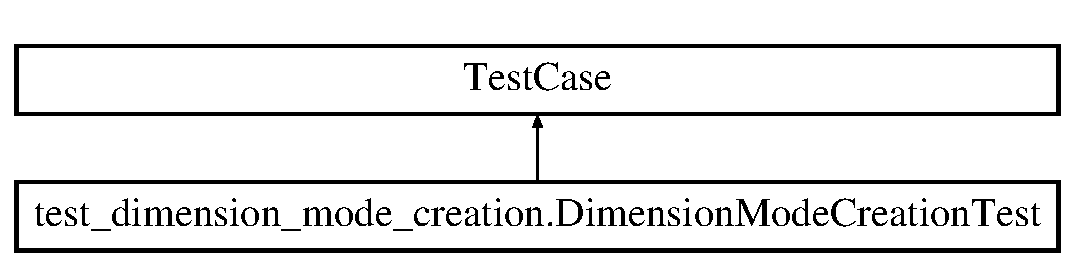
\includegraphics[height=2.000000cm]{classtest__dimension__mode__creation_1_1_dimension_mode_creation_test}
\end{center}
\end{figure}
\subsection*{Public Member Functions}
\begin{DoxyCompactItemize}
\item 
\hypertarget{classtest__dimension__mode__creation_1_1_dimension_mode_creation_test_a270636459480ac12e0c24524f5265e9f}{def {\bfseries set\-Up}}\label{classtest__dimension__mode__creation_1_1_dimension_mode_creation_test_a270636459480ac12e0c24524f5265e9f}

\item 
\hypertarget{classtest__dimension__mode__creation_1_1_dimension_mode_creation_test_a075d013032b40ae2e2ea654faf91f964}{def {\bfseries test\-\_\-random\-\_\-creation}}\label{classtest__dimension__mode__creation_1_1_dimension_mode_creation_test_a075d013032b40ae2e2ea654faf91f964}

\end{DoxyCompactItemize}
\subsection*{Public Attributes}
\begin{DoxyCompactItemize}
\item 
\hypertarget{classtest__dimension__mode__creation_1_1_dimension_mode_creation_test_a314058ecd7e18a734af6783a556aea9d}{{\bfseries config}}\label{classtest__dimension__mode__creation_1_1_dimension_mode_creation_test_a314058ecd7e18a734af6783a556aea9d}

\end{DoxyCompactItemize}


The documentation for this class was generated from the following file\-:\begin{DoxyCompactItemize}
\item 
test/test\-\_\-dimension\-\_\-mode\-\_\-creation.\-py\end{DoxyCompactItemize}

\hypertarget{classctpy_1_1data_1_1experiment__tracking_1_1_experiment_tracking}{\section{ctpy.\-data.\-experiment\-\_\-tracking.\-Experiment\-Tracking Class Reference}
\label{classctpy_1_1data_1_1experiment__tracking_1_1_experiment_tracking}\index{ctpy.\-data.\-experiment\-\_\-tracking.\-Experiment\-Tracking@{ctpy.\-data.\-experiment\-\_\-tracking.\-Experiment\-Tracking}}
}
Inheritance diagram for ctpy.\-data.\-experiment\-\_\-tracking.\-Experiment\-Tracking\-:\begin{figure}[H]
\begin{center}
\leavevmode
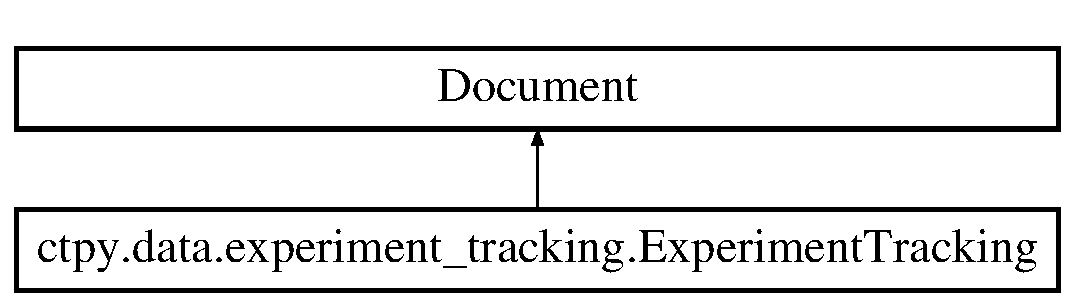
\includegraphics[height=2.000000cm]{classctpy_1_1data_1_1experiment__tracking_1_1_experiment_tracking}
\end{center}
\end{figure}
\subsection*{Classes}
\begin{DoxyCompactItemize}
\item 
class \hyperlink{classctpy_1_1data_1_1experiment__tracking_1_1_experiment_tracking_1_1____mongometa____}{\-\_\-\-\_\-mongometa\-\_\-\-\_\-}
\end{DoxyCompactItemize}
\subsection*{Static Public Attributes}
\begin{DoxyCompactItemize}
\item 
\hypertarget{classctpy_1_1data_1_1experiment__tracking_1_1_experiment_tracking_a11a6ddd6e390436eaac0c7f3dd2e590a}{tuple {\bfseries experiment\-\_\-name} = Field(str)}\label{classctpy_1_1data_1_1experiment__tracking_1_1_experiment_tracking_a11a6ddd6e390436eaac0c7f3dd2e590a}

\item 
\hypertarget{classctpy_1_1data_1_1experiment__tracking_1_1_experiment_tracking_a01d55d64424436fef833ea6ee8423b8c}{tuple {\bfseries experiment\-\_\-begin\-\_\-tstamp} = Field(datetime)}\label{classctpy_1_1data_1_1experiment__tracking_1_1_experiment_tracking_a01d55d64424436fef833ea6ee8423b8c}

\item 
\hypertarget{classctpy_1_1data_1_1experiment__tracking_1_1_experiment_tracking_ae7f01b7af62a12d733e16e4c55be51fb}{tuple {\bfseries description} = Field(str)}\label{classctpy_1_1data_1_1experiment__tracking_1_1_experiment_tracking_ae7f01b7af62a12d733e16e4c55be51fb}

\item 
\hypertarget{classctpy_1_1data_1_1experiment__tracking_1_1_experiment_tracking_a9ee1c729744f4a30e30323d9ba66a443}{tuple {\bfseries sim\-\_\-data\-\_\-collected} = Field(bool)}\label{classctpy_1_1data_1_1experiment__tracking_1_1_experiment_tracking_a9ee1c729744f4a30e30323d9ba66a443}

\item 
\hypertarget{classctpy_1_1data_1_1experiment__tracking_1_1_experiment_tracking_ade8ab199d56941ac98d041efb4871b53}{tuple {\bfseries sim\-\_\-data\-\_\-tstamp} = Field(datetime)}\label{classctpy_1_1data_1_1experiment__tracking_1_1_experiment_tracking_ade8ab199d56941ac98d041efb4871b53}

\item 
\hypertarget{classctpy_1_1data_1_1experiment__tracking_1_1_experiment_tracking_a6be2aaee1fc4b82bd6f145d765e9fe19}{tuple {\bfseries subsampling\-\_\-complete} = Field(bool)}\label{classctpy_1_1data_1_1experiment__tracking_1_1_experiment_tracking_a6be2aaee1fc4b82bd6f145d765e9fe19}

\item 
\hypertarget{classctpy_1_1data_1_1experiment__tracking_1_1_experiment_tracking_a598be75ac627f12e13aac7bd92abfbc0}{tuple {\bfseries subsampling\-\_\-tstamp} = Field(datetime)}\label{classctpy_1_1data_1_1experiment__tracking_1_1_experiment_tracking_a598be75ac627f12e13aac7bd92abfbc0}

\item 
\hypertarget{classctpy_1_1data_1_1experiment__tracking_1_1_experiment_tracking_a14ad63655e4b950f99e93aad80e885b0}{tuple {\bfseries classification\-\_\-complete} = Field(bool)}\label{classctpy_1_1data_1_1experiment__tracking_1_1_experiment_tracking_a14ad63655e4b950f99e93aad80e885b0}

\item 
\hypertarget{classctpy_1_1data_1_1experiment__tracking_1_1_experiment_tracking_a24101514fc68b9f3f668a94e7fc8c83e}{tuple {\bfseries classification\-\_\-tstamp} = Field(datetime)}\label{classctpy_1_1data_1_1experiment__tracking_1_1_experiment_tracking_a24101514fc68b9f3f668a94e7fc8c83e}

\item 
\hypertarget{classctpy_1_1data_1_1experiment__tracking_1_1_experiment_tracking_a106950435a85af9924a006cfb398221e}{tuple {\bfseries postclassification\-\_\-simrun\-\_\-stats\-\_\-complete} = Field(bool)}\label{classctpy_1_1data_1_1experiment__tracking_1_1_experiment_tracking_a106950435a85af9924a006cfb398221e}

\item 
\hypertarget{classctpy_1_1data_1_1experiment__tracking_1_1_experiment_tracking_a239be38dc51505a336eb9dcb7a624906}{tuple {\bfseries postclassification\-\_\-simrun\-\_\-stats\-\_\-tstamp} = Field(datetime)}\label{classctpy_1_1data_1_1experiment__tracking_1_1_experiment_tracking_a239be38dc51505a336eb9dcb7a624906}

\item 
\hypertarget{classctpy_1_1data_1_1experiment__tracking_1_1_experiment_tracking_a39a44da7a732920a3a46f5425e6d3226}{tuple {\bfseries timeaveraging\-\_\-complete} = Field(bool)}\label{classctpy_1_1data_1_1experiment__tracking_1_1_experiment_tracking_a39a44da7a732920a3a46f5425e6d3226}

\item 
\hypertarget{classctpy_1_1data_1_1experiment__tracking_1_1_experiment_tracking_a630e57bcbffb4fedd747c4c17cc433f5}{tuple {\bfseries timeaveraging\-\_\-tstamp} = Field(datetime)}\label{classctpy_1_1data_1_1experiment__tracking_1_1_experiment_tracking_a630e57bcbffb4fedd747c4c17cc433f5}

\item 
\hypertarget{classctpy_1_1data_1_1experiment__tracking_1_1_experiment_tracking_ab2e1e717321525dc37770425a81f2080}{tuple {\bfseries ta\-\_\-classification\-\_\-complete} = Field(bool)}\label{classctpy_1_1data_1_1experiment__tracking_1_1_experiment_tracking_ab2e1e717321525dc37770425a81f2080}

\item 
\hypertarget{classctpy_1_1data_1_1experiment__tracking_1_1_experiment_tracking_a0d1d93c5e5027d9413face9446ccb3da}{tuple {\bfseries ta\-\_\-classification\-\_\-tstamp} = Field(datetime)}\label{classctpy_1_1data_1_1experiment__tracking_1_1_experiment_tracking_a0d1d93c5e5027d9413face9446ccb3da}

\item 
\hypertarget{classctpy_1_1data_1_1experiment__tracking_1_1_experiment_tracking_a0190e75dcf9cd377b6e77eb223d00c5c}{tuple {\bfseries trait\-\_\-statistics\-\_\-complete} = Field(bool)}\label{classctpy_1_1data_1_1experiment__tracking_1_1_experiment_tracking_a0190e75dcf9cd377b6e77eb223d00c5c}

\item 
\hypertarget{classctpy_1_1data_1_1experiment__tracking_1_1_experiment_tracking_a59413bb77b9bb4035b06f28afae0f14d}{tuple {\bfseries trait\-\_\-statistics\-\_\-tstamp} = Field(datetime)}\label{classctpy_1_1data_1_1experiment__tracking_1_1_experiment_tracking_a59413bb77b9bb4035b06f28afae0f14d}

\item 
\hypertarget{classctpy_1_1data_1_1experiment__tracking_1_1_experiment_tracking_a9991f135d33eda5fe80d1290f90a96b3}{tuple {\bfseries experiment\-\_\-end\-\_\-processing\-\_\-time} = Field(datetime)}\label{classctpy_1_1data_1_1experiment__tracking_1_1_experiment_tracking_a9991f135d33eda5fe80d1290f90a96b3}

\end{DoxyCompactItemize}


The documentation for this class was generated from the following file\-:\begin{DoxyCompactItemize}
\item 
ctpy/data/experiment\-\_\-tracking.\-py\end{DoxyCompactItemize}

\hypertarget{classctpy_1_1data_1_1individual__sample_1_1_individual_sample}{\section{ctpy.\-data.\-individual\-\_\-sample.\-Individual\-Sample Class Reference}
\label{classctpy_1_1data_1_1individual__sample_1_1_individual_sample}\index{ctpy.\-data.\-individual\-\_\-sample.\-Individual\-Sample@{ctpy.\-data.\-individual\-\_\-sample.\-Individual\-Sample}}
}
Inheritance diagram for ctpy.\-data.\-individual\-\_\-sample.\-Individual\-Sample\-:\begin{figure}[H]
\begin{center}
\leavevmode
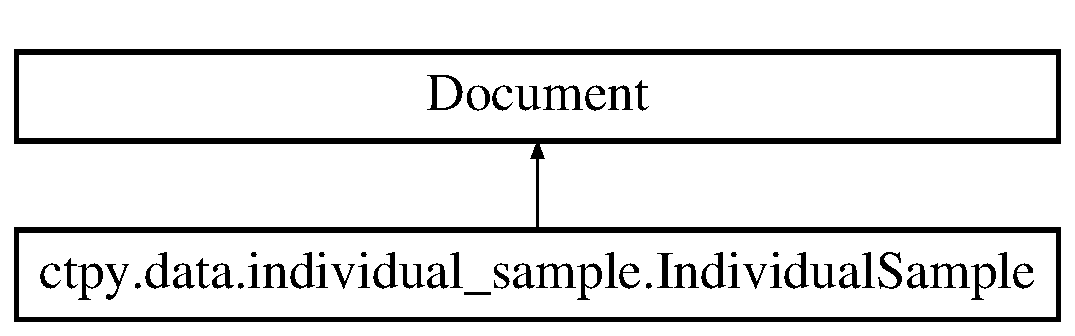
\includegraphics[height=2.000000cm]{classctpy_1_1data_1_1individual__sample_1_1_individual_sample}
\end{center}
\end{figure}
\subsection*{Classes}
\begin{DoxyCompactItemize}
\item 
class \hyperlink{classctpy_1_1data_1_1individual__sample_1_1_individual_sample_1_1____mongometa____}{\-\_\-\-\_\-mongometa\-\_\-\-\_\-}
\end{DoxyCompactItemize}


The documentation for this class was generated from the following file\-:\begin{DoxyCompactItemize}
\item 
ctpy/data/individual\-\_\-sample.\-py\end{DoxyCompactItemize}

\hypertarget{classctpy_1_1data_1_1individual__sample__classified_1_1_individual_sample_classified}{\section{ctpy.\-data.\-individual\-\_\-sample\-\_\-classified.\-Individual\-Sample\-Classified Class Reference}
\label{classctpy_1_1data_1_1individual__sample__classified_1_1_individual_sample_classified}\index{ctpy.\-data.\-individual\-\_\-sample\-\_\-classified.\-Individual\-Sample\-Classified@{ctpy.\-data.\-individual\-\_\-sample\-\_\-classified.\-Individual\-Sample\-Classified}}
}
Inheritance diagram for ctpy.\-data.\-individual\-\_\-sample\-\_\-classified.\-Individual\-Sample\-Classified\-:\begin{figure}[H]
\begin{center}
\leavevmode
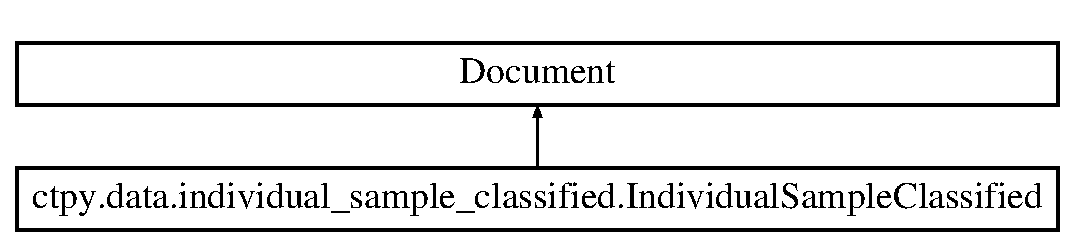
\includegraphics[height=2.000000cm]{classctpy_1_1data_1_1individual__sample__classified_1_1_individual_sample_classified}
\end{center}
\end{figure}
\subsection*{Classes}
\begin{DoxyCompactItemize}
\item 
class \hyperlink{classctpy_1_1data_1_1individual__sample__classified_1_1_individual_sample_classified_1_1____mongometa____}{\-\_\-\-\_\-mongometa\-\_\-\-\_\-}
\end{DoxyCompactItemize}


The documentation for this class was generated from the following file\-:\begin{DoxyCompactItemize}
\item 
ctpy/data/individual\-\_\-sample\-\_\-classified.\-py\end{DoxyCompactItemize}

\hypertarget{classctpy_1_1data_1_1individual__sample__fulldataset_1_1_individual_sample_full_dataset}{\section{ctpy.\-data.\-individual\-\_\-sample\-\_\-fulldataset.\-Individual\-Sample\-Full\-Dataset Class Reference}
\label{classctpy_1_1data_1_1individual__sample__fulldataset_1_1_individual_sample_full_dataset}\index{ctpy.\-data.\-individual\-\_\-sample\-\_\-fulldataset.\-Individual\-Sample\-Full\-Dataset@{ctpy.\-data.\-individual\-\_\-sample\-\_\-fulldataset.\-Individual\-Sample\-Full\-Dataset}}
}
Inheritance diagram for ctpy.\-data.\-individual\-\_\-sample\-\_\-fulldataset.\-Individual\-Sample\-Full\-Dataset\-:\begin{figure}[H]
\begin{center}
\leavevmode
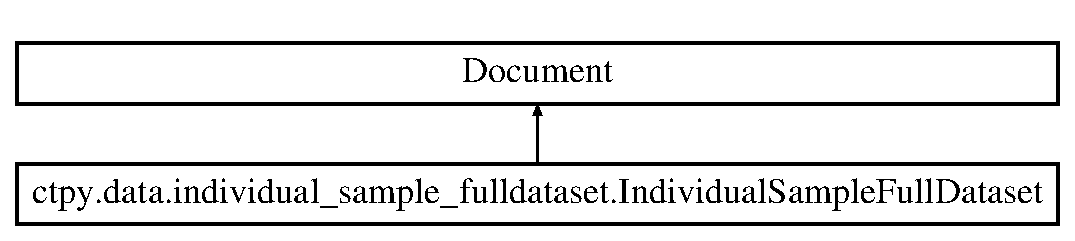
\includegraphics[height=2.000000cm]{classctpy_1_1data_1_1individual__sample__fulldataset_1_1_individual_sample_full_dataset}
\end{center}
\end{figure}
\subsection*{Classes}
\begin{DoxyCompactItemize}
\item 
class \hyperlink{classctpy_1_1data_1_1individual__sample__fulldataset_1_1_individual_sample_full_dataset_1_1____mongometa____}{\-\_\-\-\_\-mongometa\-\_\-\-\_\-}
\end{DoxyCompactItemize}


The documentation for this class was generated from the following file\-:\begin{DoxyCompactItemize}
\item 
ctpy/data/individual\-\_\-sample\-\_\-fulldataset.\-py\end{DoxyCompactItemize}

\hypertarget{classctpy_1_1innovation__models_1_1simple__mutators_1_1_k_allele_lifetime_tracking_mutator}{\section{ctpy.\-innovation\-\_\-models.\-simple\-\_\-mutators.\-K\-Allele\-Lifetime\-Tracking\-Mutator Class Reference}
\label{classctpy_1_1innovation__models_1_1simple__mutators_1_1_k_allele_lifetime_tracking_mutator}\index{ctpy.\-innovation\-\_\-models.\-simple\-\_\-mutators.\-K\-Allele\-Lifetime\-Tracking\-Mutator@{ctpy.\-innovation\-\_\-models.\-simple\-\_\-mutators.\-K\-Allele\-Lifetime\-Tracking\-Mutator}}
}
Inheritance diagram for ctpy.\-innovation\-\_\-models.\-simple\-\_\-mutators.\-K\-Allele\-Lifetime\-Tracking\-Mutator\-:\begin{figure}[H]
\begin{center}
\leavevmode
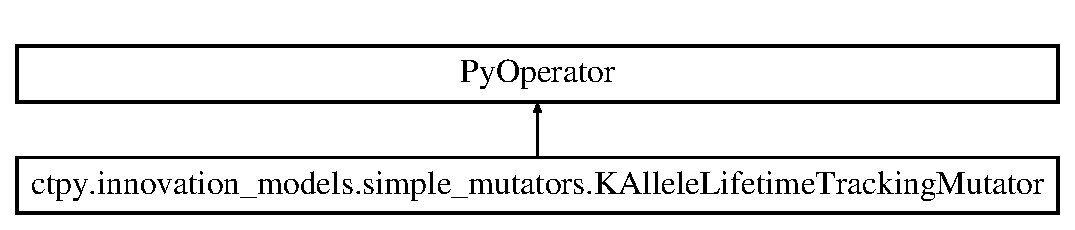
\includegraphics[height=2.000000cm]{classctpy_1_1innovation__models_1_1simple__mutators_1_1_k_allele_lifetime_tracking_mutator}
\end{center}
\end{figure}
\subsection*{Public Member Functions}
\begin{DoxyCompactItemize}
\item 
\hypertarget{classctpy_1_1innovation__models_1_1simple__mutators_1_1_k_allele_lifetime_tracking_mutator_a382c3c821858fcc554d4d97788f986c7}{def {\bfseries \-\_\-\-\_\-init\-\_\-\-\_\-}}\label{classctpy_1_1innovation__models_1_1simple__mutators_1_1_k_allele_lifetime_tracking_mutator_a382c3c821858fcc554d4d97788f986c7}

\item 
\hypertarget{classctpy_1_1innovation__models_1_1simple__mutators_1_1_k_allele_lifetime_tracking_mutator_a08c1d80f4c8dbbda11b7a989cde703af}{def {\bfseries mutate}}\label{classctpy_1_1innovation__models_1_1simple__mutators_1_1_k_allele_lifetime_tracking_mutator_a08c1d80f4c8dbbda11b7a989cde703af}

\end{DoxyCompactItemize}
\subsection*{Public Attributes}
\begin{DoxyCompactItemize}
\item 
\hypertarget{classctpy_1_1innovation__models_1_1simple__mutators_1_1_k_allele_lifetime_tracking_mutator_a520255f4c4c432dec6a359f3fbe43e2c}{{\bfseries k}}\label{classctpy_1_1innovation__models_1_1simple__mutators_1_1_k_allele_lifetime_tracking_mutator_a520255f4c4c432dec6a359f3fbe43e2c}

\item 
\hypertarget{classctpy_1_1innovation__models_1_1simple__mutators_1_1_k_allele_lifetime_tracking_mutator_a0e1450702578e2e363e0b2950cf0eb5b}{{\bfseries rates}}\label{classctpy_1_1innovation__models_1_1simple__mutators_1_1_k_allele_lifetime_tracking_mutator_a0e1450702578e2e363e0b2950cf0eb5b}

\item 
\hypertarget{classctpy_1_1innovation__models_1_1simple__mutators_1_1_k_allele_lifetime_tracking_mutator_acb611732a2906165e25c5b0a324d8683}{{\bfseries loci}}\label{classctpy_1_1innovation__models_1_1simple__mutators_1_1_k_allele_lifetime_tracking_mutator_acb611732a2906165e25c5b0a324d8683}

\end{DoxyCompactItemize}


The documentation for this class was generated from the following file\-:\begin{DoxyCompactItemize}
\item 
ctpy/innovation\-\_\-models/simple\-\_\-mutators.\-py\end{DoxyCompactItemize}

\hypertarget{classtest__math_1_1_math_test}{\section{test\-\_\-math.\-Math\-Test Class Reference}
\label{classtest__math_1_1_math_test}\index{test\-\_\-math.\-Math\-Test@{test\-\_\-math.\-Math\-Test}}
}
Inheritance diagram for test\-\_\-math.\-Math\-Test\-:\begin{figure}[H]
\begin{center}
\leavevmode
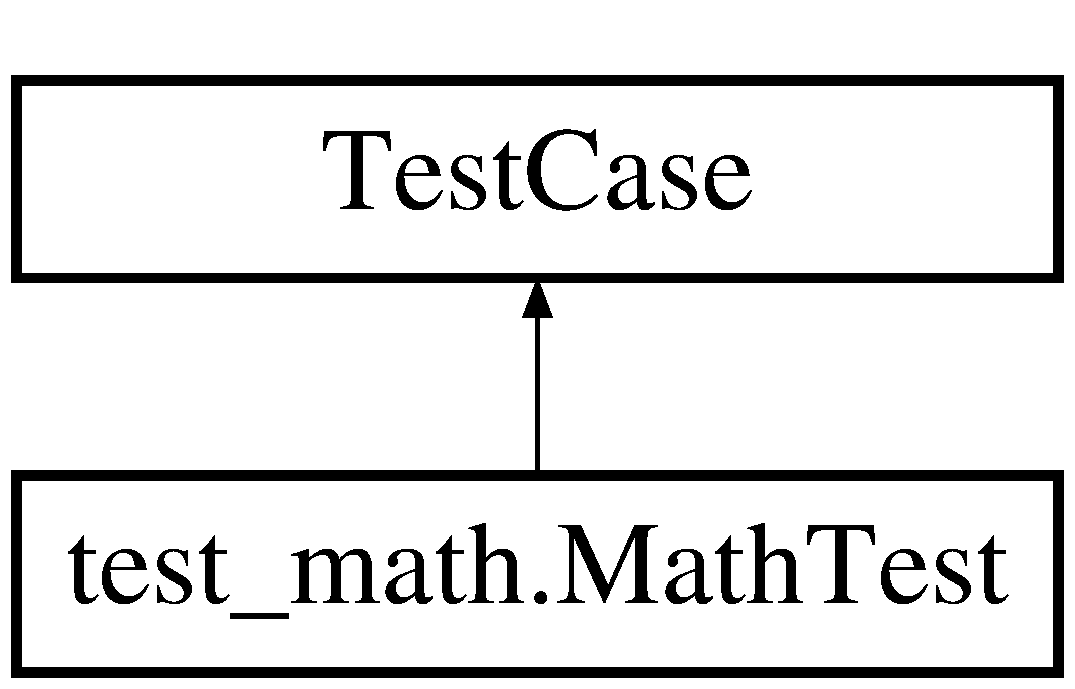
\includegraphics[height=2.000000cm]{classtest__math_1_1_math_test}
\end{center}
\end{figure}
\subsection*{Public Member Functions}
\begin{DoxyCompactItemize}
\item 
\hypertarget{classtest__math_1_1_math_test_a17a48883f0f84b75af8bd91d68fcb941}{def {\bfseries test\-\_\-expected\-Time\-Stationarity\-Haploid}}\label{classtest__math_1_1_math_test_a17a48883f0f84b75af8bd91d68fcb941}

\end{DoxyCompactItemize}


The documentation for this class was generated from the following file\-:\begin{DoxyCompactItemize}
\item 
test/test\-\_\-math.\-py\end{DoxyCompactItemize}

\hypertarget{classctpy_1_1data_1_1pergeneration__stats__postclassification_1_1_per_generation_stats_postclassification}{\section{ctpy.\-data.\-pergeneration\-\_\-stats\-\_\-postclassification.\-Per\-Generation\-Stats\-Postclassification Class Reference}
\label{classctpy_1_1data_1_1pergeneration__stats__postclassification_1_1_per_generation_stats_postclassification}\index{ctpy.\-data.\-pergeneration\-\_\-stats\-\_\-postclassification.\-Per\-Generation\-Stats\-Postclassification@{ctpy.\-data.\-pergeneration\-\_\-stats\-\_\-postclassification.\-Per\-Generation\-Stats\-Postclassification}}
}
Inheritance diagram for ctpy.\-data.\-pergeneration\-\_\-stats\-\_\-postclassification.\-Per\-Generation\-Stats\-Postclassification\-:\begin{figure}[H]
\begin{center}
\leavevmode
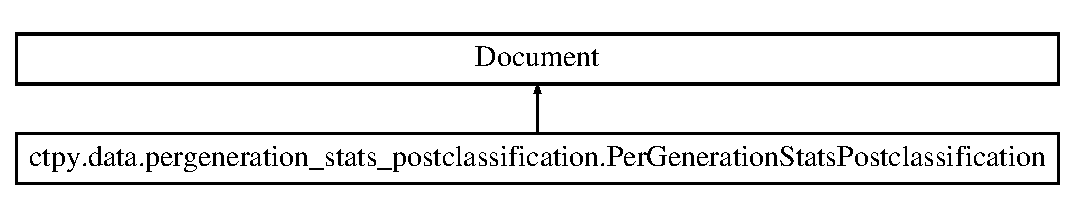
\includegraphics[height=2.000000cm]{classctpy_1_1data_1_1pergeneration__stats__postclassification_1_1_per_generation_stats_postclassification}
\end{center}
\end{figure}
\subsection*{Classes}
\begin{DoxyCompactItemize}
\item 
class \hyperlink{classctpy_1_1data_1_1pergeneration__stats__postclassification_1_1_per_generation_stats_postclassification_1_1____mongometa____}{\-\_\-\-\_\-mongometa\-\_\-\-\_\-}
\end{DoxyCompactItemize}


The documentation for this class was generated from the following file\-:\begin{DoxyCompactItemize}
\item 
ctpy/data/pergeneration\-\_\-stats\-\_\-postclassification.\-py\end{DoxyCompactItemize}

\hypertarget{classctpy_1_1data_1_1pergeneration__stats__traits_1_1_per_generation_stats_traits}{\section{ctpy.\-data.\-pergeneration\-\_\-stats\-\_\-traits.\-Per\-Generation\-Stats\-Traits Class Reference}
\label{classctpy_1_1data_1_1pergeneration__stats__traits_1_1_per_generation_stats_traits}\index{ctpy.\-data.\-pergeneration\-\_\-stats\-\_\-traits.\-Per\-Generation\-Stats\-Traits@{ctpy.\-data.\-pergeneration\-\_\-stats\-\_\-traits.\-Per\-Generation\-Stats\-Traits}}
}
Inheritance diagram for ctpy.\-data.\-pergeneration\-\_\-stats\-\_\-traits.\-Per\-Generation\-Stats\-Traits\-:\begin{figure}[H]
\begin{center}
\leavevmode
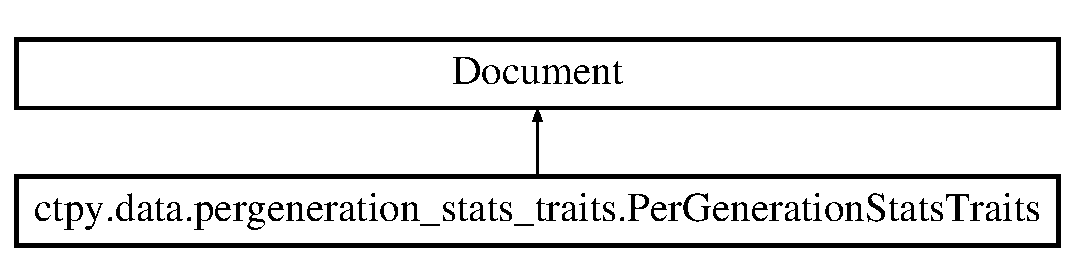
\includegraphics[height=2.000000cm]{classctpy_1_1data_1_1pergeneration__stats__traits_1_1_per_generation_stats_traits}
\end{center}
\end{figure}
\subsection*{Classes}
\begin{DoxyCompactItemize}
\item 
class \hyperlink{classctpy_1_1data_1_1pergeneration__stats__traits_1_1_per_generation_stats_traits_1_1____mongometa____}{\-\_\-\-\_\-mongometa\-\_\-\-\_\-}
\end{DoxyCompactItemize}


The documentation for this class was generated from the following file\-:\begin{DoxyCompactItemize}
\item 
ctpy/data/pergeneration\-\_\-stats\-\_\-traits.\-py\end{DoxyCompactItemize}

\hypertarget{classctpy_1_1data_1_1persimrun__stats__postclassification_1_1_per_simrun_stats_postclassification}{\section{ctpy.\-data.\-persimrun\-\_\-stats\-\_\-postclassification.\-Per\-Simrun\-Stats\-Postclassification Class Reference}
\label{classctpy_1_1data_1_1persimrun__stats__postclassification_1_1_per_simrun_stats_postclassification}\index{ctpy.\-data.\-persimrun\-\_\-stats\-\_\-postclassification.\-Per\-Simrun\-Stats\-Postclassification@{ctpy.\-data.\-persimrun\-\_\-stats\-\_\-postclassification.\-Per\-Simrun\-Stats\-Postclassification}}
}
Inheritance diagram for ctpy.\-data.\-persimrun\-\_\-stats\-\_\-postclassification.\-Per\-Simrun\-Stats\-Postclassification\-:\begin{figure}[H]
\begin{center}
\leavevmode
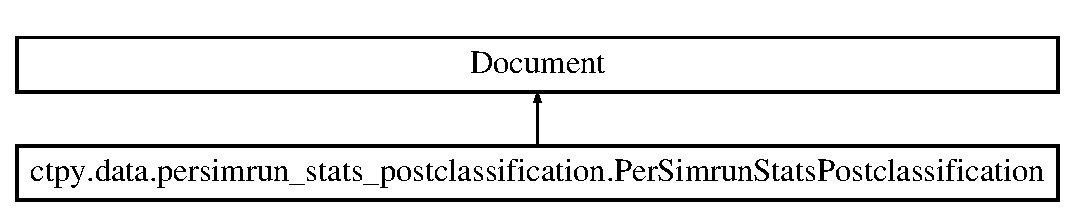
\includegraphics[height=2.000000cm]{classctpy_1_1data_1_1persimrun__stats__postclassification_1_1_per_simrun_stats_postclassification}
\end{center}
\end{figure}
\subsection*{Classes}
\begin{DoxyCompactItemize}
\item 
class \hyperlink{classctpy_1_1data_1_1persimrun__stats__postclassification_1_1_per_simrun_stats_postclassification_1_1____mongometa____}{\-\_\-\-\_\-mongometa\-\_\-\-\_\-}
\end{DoxyCompactItemize}


The documentation for this class was generated from the following file\-:\begin{DoxyCompactItemize}
\item 
ctpy/data/persimrun\-\_\-stats\-\_\-postclassification.\-py\end{DoxyCompactItemize}

\hypertarget{classctpy_1_1data_1_1richness__sample_1_1_richness_sample}{\section{ctpy.\-data.\-richness\-\_\-sample.\-Richness\-Sample Class Reference}
\label{classctpy_1_1data_1_1richness__sample_1_1_richness_sample}\index{ctpy.\-data.\-richness\-\_\-sample.\-Richness\-Sample@{ctpy.\-data.\-richness\-\_\-sample.\-Richness\-Sample}}
}
Inheritance diagram for ctpy.\-data.\-richness\-\_\-sample.\-Richness\-Sample\-:\begin{figure}[H]
\begin{center}
\leavevmode
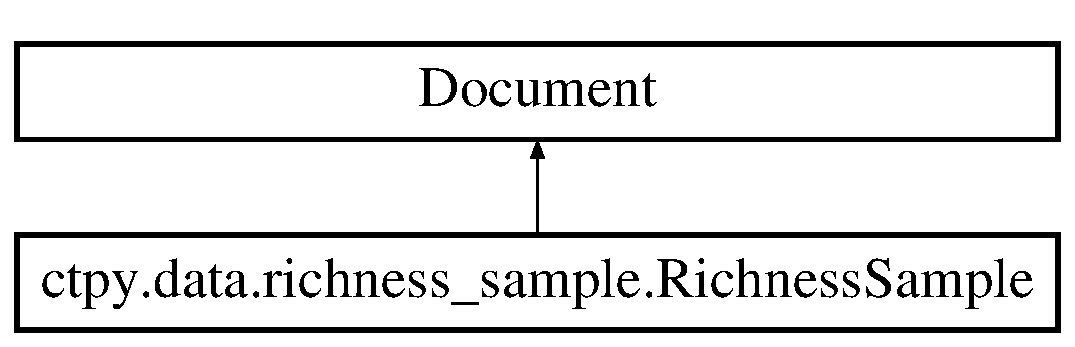
\includegraphics[height=2.000000cm]{classctpy_1_1data_1_1richness__sample_1_1_richness_sample}
\end{center}
\end{figure}
\subsection*{Classes}
\begin{DoxyCompactItemize}
\item 
class \hyperlink{classctpy_1_1data_1_1richness__sample_1_1_richness_sample_1_1____mongometa____}{\-\_\-\-\_\-mongometa\-\_\-\-\_\-}
\end{DoxyCompactItemize}
\subsection*{Static Public Attributes}
\begin{DoxyCompactItemize}
\item 
\hypertarget{classctpy_1_1data_1_1richness__sample_1_1_richness_sample_a68eb673c08d6805ec7cbf3a3e7068b46}{tuple {\bfseries simulation\-\_\-time} = Field(int)}\label{classctpy_1_1data_1_1richness__sample_1_1_richness_sample_a68eb673c08d6805ec7cbf3a3e7068b46}

\item 
\hypertarget{classctpy_1_1data_1_1richness__sample_1_1_richness_sample_a1e9a60f41a65d8dfa0d4a339705e9747}{tuple {\bfseries replication} = Field(int)}\label{classctpy_1_1data_1_1richness__sample_1_1_richness_sample_a1e9a60f41a65d8dfa0d4a339705e9747}

\item 
\hypertarget{classctpy_1_1data_1_1richness__sample_1_1_richness_sample_a6612fa63c3dea6f498a046b50bf90c5f}{tuple {\bfseries locus} = Field(int)}\label{classctpy_1_1data_1_1richness__sample_1_1_richness_sample_a6612fa63c3dea6f498a046b50bf90c5f}

\item 
\hypertarget{classctpy_1_1data_1_1richness__sample_1_1_richness_sample_a12d73e9a2988f502470749a553d3c391}{tuple {\bfseries richness} = Field(int)}\label{classctpy_1_1data_1_1richness__sample_1_1_richness_sample_a12d73e9a2988f502470749a553d3c391}

\item 
\hypertarget{classctpy_1_1data_1_1richness__sample_1_1_richness_sample_a237b768196934d75e3ce25ccc46855f1}{tuple {\bfseries sample\-\_\-size} = Field(int)}\label{classctpy_1_1data_1_1richness__sample_1_1_richness_sample_a237b768196934d75e3ce25ccc46855f1}

\item 
\hypertarget{classctpy_1_1data_1_1richness__sample_1_1_richness_sample_aa520a15eb11320d2c6e9745d09a93eb3}{tuple {\bfseries population\-\_\-size} = Field(int)}\label{classctpy_1_1data_1_1richness__sample_1_1_richness_sample_aa520a15eb11320d2c6e9745d09a93eb3}

\item 
\hypertarget{classctpy_1_1data_1_1richness__sample_1_1_richness_sample_a61f176e0fc3d53500c1797e45690bee6}{tuple {\bfseries mutation\-\_\-rate} = Field(float)}\label{classctpy_1_1data_1_1richness__sample_1_1_richness_sample_a61f176e0fc3d53500c1797e45690bee6}

\item 
\hypertarget{classctpy_1_1data_1_1richness__sample_1_1_richness_sample_a1867be6ea892d9b5d7b33a7135707556}{tuple {\bfseries simulation\-\_\-run\-\_\-id} = Field(str)}\label{classctpy_1_1data_1_1richness__sample_1_1_richness_sample_a1867be6ea892d9b5d7b33a7135707556}

\end{DoxyCompactItemize}


The documentation for this class was generated from the following file\-:\begin{DoxyCompactItemize}
\item 
ctpy/data/richness\-\_\-sample.\-py\end{DoxyCompactItemize}

\hypertarget{classctpy_1_1data_1_1richness__population_1_1_richness_sample}{\section{ctpy.\-data.\-richness\-\_\-population.\-Richness\-Sample Class Reference}
\label{classctpy_1_1data_1_1richness__population_1_1_richness_sample}\index{ctpy.\-data.\-richness\-\_\-population.\-Richness\-Sample@{ctpy.\-data.\-richness\-\_\-population.\-Richness\-Sample}}
}
Inheritance diagram for ctpy.\-data.\-richness\-\_\-population.\-Richness\-Sample\-:\begin{figure}[H]
\begin{center}
\leavevmode
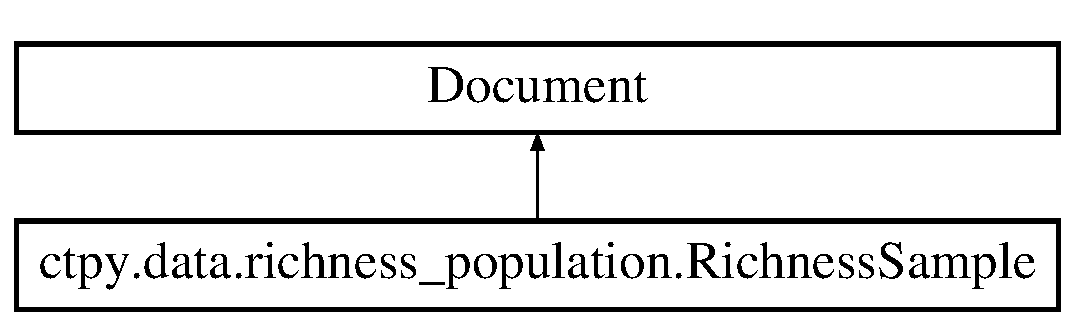
\includegraphics[height=2.000000cm]{classctpy_1_1data_1_1richness__population_1_1_richness_sample}
\end{center}
\end{figure}
\subsection*{Classes}
\begin{DoxyCompactItemize}
\item 
class \hyperlink{classctpy_1_1data_1_1richness__population_1_1_richness_sample_1_1____mongometa____}{\-\_\-\-\_\-mongometa\-\_\-\-\_\-}
\end{DoxyCompactItemize}
\subsection*{Static Public Attributes}
\begin{DoxyCompactItemize}
\item 
\hypertarget{classctpy_1_1data_1_1richness__population_1_1_richness_sample_a2ab22098b5717c5e6b56111a257c6d65}{tuple {\bfseries simulation\-\_\-time} = Field(int)}\label{classctpy_1_1data_1_1richness__population_1_1_richness_sample_a2ab22098b5717c5e6b56111a257c6d65}

\item 
\hypertarget{classctpy_1_1data_1_1richness__population_1_1_richness_sample_aa52e6656d0ee603c7fa8839a73bdbc81}{tuple {\bfseries replication} = Field(int)}\label{classctpy_1_1data_1_1richness__population_1_1_richness_sample_aa52e6656d0ee603c7fa8839a73bdbc81}

\item 
\hypertarget{classctpy_1_1data_1_1richness__population_1_1_richness_sample_a11d69ad62eb0cfea1398ab07f382c3dd}{tuple {\bfseries locus} = Field(int)}\label{classctpy_1_1data_1_1richness__population_1_1_richness_sample_a11d69ad62eb0cfea1398ab07f382c3dd}

\item 
\hypertarget{classctpy_1_1data_1_1richness__population_1_1_richness_sample_aa8f49f1cb4f8e79f8e869708ccc131f0}{tuple {\bfseries richness} = Field(int)}\label{classctpy_1_1data_1_1richness__population_1_1_richness_sample_aa8f49f1cb4f8e79f8e869708ccc131f0}

\item 
\hypertarget{classctpy_1_1data_1_1richness__population_1_1_richness_sample_a7a32f3ee38da08e1291b114c219dc658}{tuple {\bfseries population\-\_\-size} = Field(int)}\label{classctpy_1_1data_1_1richness__population_1_1_richness_sample_a7a32f3ee38da08e1291b114c219dc658}

\item 
\hypertarget{classctpy_1_1data_1_1richness__population_1_1_richness_sample_aa98cb410fba2165a8e9cf07a7adeedd0}{tuple {\bfseries mutation\-\_\-rate} = Field(float)}\label{classctpy_1_1data_1_1richness__population_1_1_richness_sample_aa98cb410fba2165a8e9cf07a7adeedd0}

\item 
\hypertarget{classctpy_1_1data_1_1richness__population_1_1_richness_sample_ace79f1b9c235fb93832961547fd5c851}{tuple {\bfseries simulation\-\_\-run\-\_\-id} = Field(str)}\label{classctpy_1_1data_1_1richness__population_1_1_richness_sample_ace79f1b9c235fb93832961547fd5c851}

\end{DoxyCompactItemize}


The documentation for this class was generated from the following file\-:\begin{DoxyCompactItemize}
\item 
ctpy/data/richness\-\_\-population.\-py\end{DoxyCompactItemize}

\hypertarget{classtest__sampling_1_1_sampling_test}{\section{test\-\_\-sampling.\-Sampling\-Test Class Reference}
\label{classtest__sampling_1_1_sampling_test}\index{test\-\_\-sampling.\-Sampling\-Test@{test\-\_\-sampling.\-Sampling\-Test}}
}
Inheritance diagram for test\-\_\-sampling.\-Sampling\-Test\-:\begin{figure}[H]
\begin{center}
\leavevmode
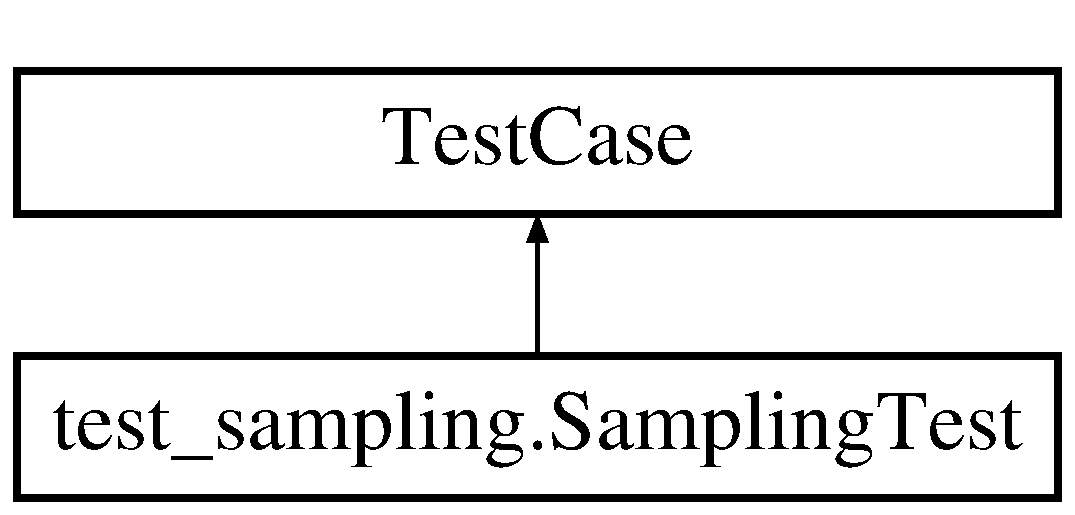
\includegraphics[height=2.000000cm]{classtest__sampling_1_1_sampling_test}
\end{center}
\end{figure}
\subsection*{Public Member Functions}
\begin{DoxyCompactItemize}
\item 
\hypertarget{classtest__sampling_1_1_sampling_test_a6f817a84e2cea300d82d21afea82dbd3}{def {\bfseries test\-\_\-ewens\-\_\-sample}}\label{classtest__sampling_1_1_sampling_test_a6f817a84e2cea300d82d21afea82dbd3}

\end{DoxyCompactItemize}


The documentation for this class was generated from the following file\-:\begin{DoxyCompactItemize}
\item 
test/test\-\_\-sampling.\-py\end{DoxyCompactItemize}

\hypertarget{classctpy_1_1utils_1_1script__args_1_1_script_args}{\section{ctpy.\-utils.\-script\-\_\-args.\-Script\-Args Class Reference}
\label{classctpy_1_1utils_1_1script__args_1_1_script_args}\index{ctpy.\-utils.\-script\-\_\-args.\-Script\-Args@{ctpy.\-utils.\-script\-\_\-args.\-Script\-Args}}
}
\subsection*{Public Member Functions}
\begin{DoxyCompactItemize}
\item 
\hypertarget{classctpy_1_1utils_1_1script__args_1_1_script_args_afa6de6722a57b8cffcbb772508024887}{def {\bfseries \-\_\-\-\_\-init\-\_\-\-\_\-}}\label{classctpy_1_1utils_1_1script__args_1_1_script_args_afa6de6722a57b8cffcbb772508024887}

\end{DoxyCompactItemize}
\subsection*{Public Attributes}
\begin{DoxyCompactItemize}
\item 
\hypertarget{classctpy_1_1utils_1_1script__args_1_1_script_args_a8190230c34ea72ccbdb53736f54ad21d}{{\bfseries experiment\-\_\-name}}\label{classctpy_1_1utils_1_1script__args_1_1_script_args_a8190230c34ea72ccbdb53736f54ad21d}

\item 
\hypertarget{classctpy_1_1utils_1_1script__args_1_1_script_args_a1a54fcb34e30a94ac8f23751ee71ce4f}{{\bfseries database\-\_\-hostname}}\label{classctpy_1_1utils_1_1script__args_1_1_script_args_a1a54fcb34e30a94ac8f23751ee71ce4f}

\item 
\hypertarget{classctpy_1_1utils_1_1script__args_1_1_script_args_a55db3e14c5abf387d141092e4571f266}{{\bfseries database\-\_\-port}}\label{classctpy_1_1utils_1_1script__args_1_1_script_args_a55db3e14c5abf387d141092e4571f266}

\item 
\hypertarget{classctpy_1_1utils_1_1script__args_1_1_script_args_afbe19af07ce4af333ab71969472e75d4}{{\bfseries classification\-\_\-list}}\label{classctpy_1_1utils_1_1script__args_1_1_script_args_afbe19af07ce4af333ab71969472e75d4}

\item 
\hypertarget{classctpy_1_1utils_1_1script__args_1_1_script_args_a5abc22ae880888339a07eff349d69ea0}{{\bfseries parallelization}}\label{classctpy_1_1utils_1_1script__args_1_1_script_args_a5abc22ae880888339a07eff349d69ea0}

\end{DoxyCompactItemize}
\subsection*{Static Public Attributes}
\begin{DoxyCompactItemize}
\item 
\hypertarget{classctpy_1_1utils_1_1script__args_1_1_script_args_af8bc17ca882862f169e6aee8d37fb345}{{\bfseries debug} = False}\label{classctpy_1_1utils_1_1script__args_1_1_script_args_af8bc17ca882862f169e6aee8d37fb345}

\item 
\hypertarget{classctpy_1_1utils_1_1script__args_1_1_script_args_a241e38cac36cd44efdb406c71e1f5b79}{string {\bfseries experiment\-\_\-name} = \char`\"{}default\char`\"{}}\label{classctpy_1_1utils_1_1script__args_1_1_script_args_a241e38cac36cd44efdb406c71e1f5b79}

\item 
\hypertarget{classctpy_1_1utils_1_1script__args_1_1_script_args_a0f9df5a18b78baaba90299af4a629c91}{string {\bfseries database\-\_\-hostname} = \char`\"{}localhost\char`\"{}}\label{classctpy_1_1utils_1_1script__args_1_1_script_args_a0f9df5a18b78baaba90299af4a629c91}

\item 
\hypertarget{classctpy_1_1utils_1_1script__args_1_1_script_args_a7f2ddcc4e3fd25b29e8456d871e5df71}{string {\bfseries database\-\_\-port} = \char`\"{}27017\char`\"{}}\label{classctpy_1_1utils_1_1script__args_1_1_script_args_a7f2ddcc4e3fd25b29e8456d871e5df71}

\item 
\hypertarget{classctpy_1_1utils_1_1script__args_1_1_script_args_a8f943aaed17c05687c6c82f3f77743d4}{list {\bfseries classification\-\_\-list} = \mbox{[}$\,$\mbox{]}}\label{classctpy_1_1utils_1_1script__args_1_1_script_args_a8f943aaed17c05687c6c82f3f77743d4}

\item 
\hypertarget{classctpy_1_1utils_1_1script__args_1_1_script_args_adfd6a8c7df43fe35add1692f42a0b44d}{int {\bfseries parallelization} = 5}\label{classctpy_1_1utils_1_1script__args_1_1_script_args_adfd6a8c7df43fe35add1692f42a0b44d}

\item 
\hypertarget{classctpy_1_1utils_1_1script__args_1_1_script_args_a0484dd6c11a41205161489e07d0a673f}{{\bfseries configuration} = None}\label{classctpy_1_1utils_1_1script__args_1_1_script_args_a0484dd6c11a41205161489e07d0a673f}

\end{DoxyCompactItemize}


The documentation for this class was generated from the following file\-:\begin{DoxyCompactItemize}
\item 
ctpy/utils/script\-\_\-args.\-py\end{DoxyCompactItemize}

\hypertarget{classctpy_1_1math_1_1simulation__calculations_1_1_simulation_calculations}{\section{ctpy.\-math.\-simulation\-\_\-calculations.\-Simulation\-Calculations Class Reference}
\label{classctpy_1_1math_1_1simulation__calculations_1_1_simulation_calculations}\index{ctpy.\-math.\-simulation\-\_\-calculations.\-Simulation\-Calculations@{ctpy.\-math.\-simulation\-\_\-calculations.\-Simulation\-Calculations}}
}


Common Values \#\#\#\#\#\#\#\#\#\#\#\#\#.  


\subsection*{Public Member Functions}
\begin{DoxyCompactItemize}
\item 
\hypertarget{classctpy_1_1math_1_1simulation__calculations_1_1_simulation_calculations_ab00bd033de015209aba7b2e10f547d5d}{def {\bfseries \-\_\-\-\_\-init\-\_\-\-\_\-}}\label{classctpy_1_1math_1_1simulation__calculations_1_1_simulation_calculations_ab00bd033de015209aba7b2e10f547d5d}

\item 
def \hyperlink{classctpy_1_1math_1_1simulation__calculations_1_1_simulation_calculations_a26e2aee1058529d61399e51767a12460}{compute\-\_\-sim\-\_\-param\-\_\-combinations}
\begin{DoxyCompactList}\small\item\em The number of simulation parameter combinations can probably be reduced to the Cartesian product of innovation rates and overall population sizes. \end{DoxyCompactList}\item 
def \hyperlink{classctpy_1_1math_1_1simulation__calculations_1_1_simulation_calculations_af4774a281ed7c5b5c80a0440b6d12949}{compute\-\_\-even\-\_\-dimension\-\_\-classifications}
\begin{DoxyCompactList}\small\item\em Classification Combinations \#\#\#\#\#\#\#\#\#\#\#\#\#. \end{DoxyCompactList}\item 
def \hyperlink{classctpy_1_1math_1_1simulation__calculations_1_1_simulation_calculations_a8f9ffc30a7e7c68dca35021e193fcad0}{compute\-\_\-random\-\_\-dimension\-\_\-classifications}
\begin{DoxyCompactList}\small\item\em For each dimensionality, we have R classifications per level of mode partitioning M. \end{DoxyCompactList}\item 
def \hyperlink{classctpy_1_1math_1_1simulation__calculations_1_1_simulation_calculations_a8b960cd6d285a6de588321c02c00cb77}{compute\-\_\-total\-\_\-classifications}
\begin{DoxyCompactList}\small\item\em Since dimensionality is a property of subsampling the simulation output into separate data samples, any given data sample stream has a specific dimensionality (and other configuration parameters). \end{DoxyCompactList}\item 
def \hyperlink{classctpy_1_1math_1_1simulation__calculations_1_1_simulation_calculations_ad455df8e83ed3d3bc0fba5edbca5b79c}{compute\-\_\-total\-\_\-classifications\-\_\-across\-\_\-dimensionality}
\begin{DoxyCompactList}\small\item\em Sometimes we want to know how many classifications there are, across all the levels of dimensionality. \end{DoxyCompactList}\item 
def \hyperlink{classctpy_1_1math_1_1simulation__calculations_1_1_simulation_calculations_a908df80f1b75622aa3ac55786c826e45}{compute\-\_\-total\-\_\-simulation\-\_\-runs\-\_\-simple}
\begin{DoxyCompactList}\small\item\em Single Population Models (Simple Models) \#\#\#\#\#\#\#\#\#\#\#\#. \end{DoxyCompactList}\item 
def \hyperlink{classctpy_1_1math_1_1simulation__calculations_1_1_simulation_calculations_a0d1cb4ca9f1b3eb820c6c55290b54442}{compute\-\_\-total\-\_\-simulation\-\_\-replicates\-\_\-simple}
\begin{DoxyCompactList}\small\item\em For single population models, the number of simulation replicates is just the number of simulation parameter combinations times the number of simu\-P\-O\-P replicates. \end{DoxyCompactList}\item 
def \hyperlink{classctpy_1_1math_1_1simulation__calculations_1_1_simulation_calculations_aaa6bcc1a6b782731e34b9b45debd19ba}{compute\-\_\-total\-\_\-sample\-\_\-size\-\_\-replicates\-\_\-simple}
\begin{DoxyCompactList}\small\item\em For each simulation replicate in each run, we're also taking a variety of sample sizes of individuals for recording aggregate statistics and capturing genotypes for classification. \end{DoxyCompactList}\item 
def \hyperlink{classctpy_1_1math_1_1simulation__calculations_1_1_simulation_calculations_af04fd402c83c49ebeb20edbbf33371ea}{compute\-\_\-total\-\_\-replicates\-\_\-ssize\-\_\-dimensionality}
\begin{DoxyCompactList}\small\item\em From the raw sim runs, we also study different dimensionality by subsampling. \end{DoxyCompactList}\item 
def \hyperlink{classctpy_1_1math_1_1simulation__calculations_1_1_simulation_calculations_a8b4ad989ba3ccb1dcbbe74516582399c}{compute\-\_\-total\-\_\-replicates\-\_\-ssize\-\_\-dimensionality\-\_\-classifications}
\begin{DoxyCompactList}\small\item\em If we identify every replicate (given level of dimensionality, sample size, and combination of simulation parameters) with every even and random classification applicable to the given level of dimensionality, we end up with this many separate data stream samples. \end{DoxyCompactList}\item 
def \hyperlink{classctpy_1_1math_1_1simulation__calculations_1_1_simulation_calculations_a5f674e430d656ea58e8a65fecf828e89}{compute\-\_\-total\-\_\-sample\-\_\-paths\-\_\-ssize\-\_\-dim\-\_\-class\-\_\-taduration}
\begin{DoxyCompactList}\small\item\em If we aggregate raw sample paths at a variety of durations, and classify the results in addition to the raw unaggregated samples paths, this is the number of total sample paths that results. \end{DoxyCompactList}\item 
def \hyperlink{classctpy_1_1math_1_1simulation__calculations_1_1_simulation_calculations_a708d30886bbcf7f47275c068dcc48d22}{compute\-\_\-total\-\_\-number\-\_\-samples\-\_\-simple\-\_\-models}
\begin{DoxyCompactList}\small\item\em The total number of \char`\"{}samples\char`\"{} (sets of observations at a given level of ssize, dim, class, T\-A duration, simparams, replicated N times). \end{DoxyCompactList}\item 
def \hyperlink{classctpy_1_1math_1_1simulation__calculations_1_1_simulation_calculations_a0296fdc56eb45ac033f54911bd544003}{compute\-\_\-total\-\_\-number\-\_\-samples\-\_\-notimeavg\-\_\-simple\-\_\-models}
\begin{DoxyCompactList}\small\item\em For analyses with just raw samples, and no time averaging, this is the number of \char`\"{}samples\char`\"{} (sets of observations at a given level of ssize, dim, class, simparams, replicated N times). \end{DoxyCompactList}\item 
def \hyperlink{classctpy_1_1math_1_1simulation__calculations_1_1_simulation_calculations_af24f85fb2f5c2d6583d424450797e620}{compute\-\_\-network\-\_\-param\-\_\-combinations}
\begin{DoxyCompactList}\small\item\em metapopulation models \#\#\#\#\#\#\#\#\#\#\#\#\#\#\#\#\#\#\#\#\# \end{DoxyCompactList}\item 
def \hyperlink{classctpy_1_1math_1_1simulation__calculations_1_1_simulation_calculations_a80b8bc79f51913c9ec1de88f2077923f}{compute\-\_\-total\-\_\-network\-\_\-realizations}
\begin{DoxyCompactList}\small\item\em The number of network realizations is the number of network parameter combinations times the number of replicates we'll study per parameter combination. \end{DoxyCompactList}\item 
def \hyperlink{classctpy_1_1math_1_1simulation__calculations_1_1_simulation_calculations_ab4c7d2bde540dc4a98bf68030f7858b2}{compute\-\_\-total\-\_\-simulation\-\_\-runs\-\_\-metapopulation}
\begin{DoxyCompactList}\small\item\em Applicable to metapopulation models with networks of demes. \end{DoxyCompactList}\item 
def \hyperlink{classctpy_1_1math_1_1simulation__calculations_1_1_simulation_calculations_a9a2a4b527030b8870dc61c594058e8f4}{compute\-\_\-total\-\_\-simulation\-\_\-replicates\-\_\-metapopulation}
\begin{DoxyCompactList}\small\item\em Applicable to metapopulation models with networks of demes. \end{DoxyCompactList}\item 
\hypertarget{classctpy_1_1math_1_1simulation__calculations_1_1_simulation_calculations_a8ad4d81250f51646c2fc9446b2890a59}{def \hyperlink{classctpy_1_1math_1_1simulation__calculations_1_1_simulation_calculations_a8ad4d81250f51646c2fc9446b2890a59}{compute\-\_\-replicates\-\_\-ssize\-\_\-dimensionality\-\_\-metapop}}\label{classctpy_1_1math_1_1simulation__calculations_1_1_simulation_calculations_a8ad4d81250f51646c2fc9446b2890a59}

\begin{DoxyCompactList}\small\item\em \-:return\-: \end{DoxyCompactList}\item 
\hypertarget{classctpy_1_1math_1_1simulation__calculations_1_1_simulation_calculations_a1cf5ec800072697168f6e8637500d960}{def \hyperlink{classctpy_1_1math_1_1simulation__calculations_1_1_simulation_calculations_a1cf5ec800072697168f6e8637500d960}{compute\-\_\-replicates\-\_\-ssize\-\_\-dim\-\_\-classified\-\_\-metapop}}\label{classctpy_1_1math_1_1simulation__calculations_1_1_simulation_calculations_a1cf5ec800072697168f6e8637500d960}

\begin{DoxyCompactList}\small\item\em \-:return\-: \end{DoxyCompactList}\item 
\hypertarget{classctpy_1_1math_1_1simulation__calculations_1_1_simulation_calculations_a0159756aa16d7b4c2229ca4d143b05df}{def \hyperlink{classctpy_1_1math_1_1simulation__calculations_1_1_simulation_calculations_a0159756aa16d7b4c2229ca4d143b05df}{compute\-\_\-replicates\-\_\-ssize\-\_\-dim\-\_\-classified\-\_\-timeaveraged}}\label{classctpy_1_1math_1_1simulation__calculations_1_1_simulation_calculations_a0159756aa16d7b4c2229ca4d143b05df}

\begin{DoxyCompactList}\small\item\em \-:return\-: \end{DoxyCompactList}\end{DoxyCompactItemize}
\subsection*{Public Attributes}
\begin{DoxyCompactItemize}
\item 
\hypertarget{classctpy_1_1math_1_1simulation__calculations_1_1_simulation_calculations_af7970b2eae3b3acd6133b9f96373d3de}{{\bfseries simconfig}}\label{classctpy_1_1math_1_1simulation__calculations_1_1_simulation_calculations_af7970b2eae3b3acd6133b9f96373d3de}

\end{DoxyCompactItemize}


\subsection{Detailed Description}
Common Values \#\#\#\#\#\#\#\#\#\#\#\#\#. 

\subsection{Member Function Documentation}
\hypertarget{classctpy_1_1math_1_1simulation__calculations_1_1_simulation_calculations_af4774a281ed7c5b5c80a0440b6d12949}{\index{ctpy\-::math\-::simulation\-\_\-calculations\-::\-Simulation\-Calculations@{ctpy\-::math\-::simulation\-\_\-calculations\-::\-Simulation\-Calculations}!compute\-\_\-even\-\_\-dimension\-\_\-classifications@{compute\-\_\-even\-\_\-dimension\-\_\-classifications}}
\index{compute\-\_\-even\-\_\-dimension\-\_\-classifications@{compute\-\_\-even\-\_\-dimension\-\_\-classifications}!ctpy::math::simulation_calculations::SimulationCalculations@{ctpy\-::math\-::simulation\-\_\-calculations\-::\-Simulation\-Calculations}}
\subsubsection[{compute\-\_\-even\-\_\-dimension\-\_\-classifications}]{\setlength{\rightskip}{0pt plus 5cm}def ctpy.\-math.\-simulation\-\_\-calculations.\-Simulation\-Calculations.\-compute\-\_\-even\-\_\-dimension\-\_\-classifications (
\begin{DoxyParamCaption}
\item[{}]{self}
\end{DoxyParamCaption}
)}}\label{classctpy_1_1math_1_1simulation__calculations_1_1_simulation_calculations_af4774a281ed7c5b5c80a0440b6d12949}


Classification Combinations \#\#\#\#\#\#\#\#\#\#\#\#\#. 

For each dimensionality, we will have one classification per level of mode partitioning (i.\-e., a classification which chops dimensions into 2 modes, one which chops dimensions into 4 modes, etc). T\-O\-D\-O\-: We might also want classifications which are even, but different levels of partitioning for different dimensions...? \-:return\-: number of classifications with even dimensions \hypertarget{classctpy_1_1math_1_1simulation__calculations_1_1_simulation_calculations_af24f85fb2f5c2d6583d424450797e620}{\index{ctpy\-::math\-::simulation\-\_\-calculations\-::\-Simulation\-Calculations@{ctpy\-::math\-::simulation\-\_\-calculations\-::\-Simulation\-Calculations}!compute\-\_\-network\-\_\-param\-\_\-combinations@{compute\-\_\-network\-\_\-param\-\_\-combinations}}
\index{compute\-\_\-network\-\_\-param\-\_\-combinations@{compute\-\_\-network\-\_\-param\-\_\-combinations}!ctpy::math::simulation_calculations::SimulationCalculations@{ctpy\-::math\-::simulation\-\_\-calculations\-::\-Simulation\-Calculations}}
\subsubsection[{compute\-\_\-network\-\_\-param\-\_\-combinations}]{\setlength{\rightskip}{0pt plus 5cm}def ctpy.\-math.\-simulation\-\_\-calculations.\-Simulation\-Calculations.\-compute\-\_\-network\-\_\-param\-\_\-combinations (
\begin{DoxyParamCaption}
\item[{}]{self}
\end{DoxyParamCaption}
)}}\label{classctpy_1_1math_1_1simulation__calculations_1_1_simulation_calculations_af24f85fb2f5c2d6583d424450797e620}


metapopulation models \#\#\#\#\#\#\#\#\#\#\#\#\#\#\#\#\#\#\#\#\# 

The number of network model parameter combinations is important because for each combination, we will then test a number of random realizations, and each random realization will be run at all simulation parameter combinations. This value is currently the product of the levels of clustering coefficient and small-\/world rewiring probability that we're testing.

\-:return\-: number of network parameter combinations to test \hypertarget{classctpy_1_1math_1_1simulation__calculations_1_1_simulation_calculations_a8f9ffc30a7e7c68dca35021e193fcad0}{\index{ctpy\-::math\-::simulation\-\_\-calculations\-::\-Simulation\-Calculations@{ctpy\-::math\-::simulation\-\_\-calculations\-::\-Simulation\-Calculations}!compute\-\_\-random\-\_\-dimension\-\_\-classifications@{compute\-\_\-random\-\_\-dimension\-\_\-classifications}}
\index{compute\-\_\-random\-\_\-dimension\-\_\-classifications@{compute\-\_\-random\-\_\-dimension\-\_\-classifications}!ctpy::math::simulation_calculations::SimulationCalculations@{ctpy\-::math\-::simulation\-\_\-calculations\-::\-Simulation\-Calculations}}
\subsubsection[{compute\-\_\-random\-\_\-dimension\-\_\-classifications}]{\setlength{\rightskip}{0pt plus 5cm}def ctpy.\-math.\-simulation\-\_\-calculations.\-Simulation\-Calculations.\-compute\-\_\-random\-\_\-dimension\-\_\-classifications (
\begin{DoxyParamCaption}
\item[{}]{self}
\end{DoxyParamCaption}
)}}\label{classctpy_1_1math_1_1simulation__calculations_1_1_simulation_calculations_a8f9ffc30a7e7c68dca35021e193fcad0}


For each dimensionality, we have R classifications per level of mode partitioning M. 

For each of the R classifications, the M modes have random boundaries chosen uniformly. T\-O\-D\-O\-: We might want classifications which have different levels of M per dimension, but random mode boundaries....? \-:return\-: number of classifications with M mode partitions, given R randomly generated partitions per value of M \hypertarget{classctpy_1_1math_1_1simulation__calculations_1_1_simulation_calculations_a26e2aee1058529d61399e51767a12460}{\index{ctpy\-::math\-::simulation\-\_\-calculations\-::\-Simulation\-Calculations@{ctpy\-::math\-::simulation\-\_\-calculations\-::\-Simulation\-Calculations}!compute\-\_\-sim\-\_\-param\-\_\-combinations@{compute\-\_\-sim\-\_\-param\-\_\-combinations}}
\index{compute\-\_\-sim\-\_\-param\-\_\-combinations@{compute\-\_\-sim\-\_\-param\-\_\-combinations}!ctpy::math::simulation_calculations::SimulationCalculations@{ctpy\-::math\-::simulation\-\_\-calculations\-::\-Simulation\-Calculations}}
\subsubsection[{compute\-\_\-sim\-\_\-param\-\_\-combinations}]{\setlength{\rightskip}{0pt plus 5cm}def ctpy.\-math.\-simulation\-\_\-calculations.\-Simulation\-Calculations.\-compute\-\_\-sim\-\_\-param\-\_\-combinations (
\begin{DoxyParamCaption}
\item[{}]{self}
\end{DoxyParamCaption}
)}}\label{classctpy_1_1math_1_1simulation__calculations_1_1_simulation_calculations_a26e2aee1058529d61399e51767a12460}


The number of simulation parameter combinations can probably be reduced to the Cartesian product of innovation rates and overall population sizes. 

The number of trait dimensions can -- I\-F simu\-P\-O\-P evolves each locus independently in terms of mutations -- be a post-\/processing step. All \char`\"{}raw\char`\"{} simulation runs would occur with the highest number of dimensions studied (say, 8), and then to study a smaller number of dimensions (say, 2), we'd simply extract two dimensions from the raw dataset.

\-:return\-: number of simu\-P\-O\-P parameter combinations to test \hypertarget{classctpy_1_1math_1_1simulation__calculations_1_1_simulation_calculations_a8b960cd6d285a6de588321c02c00cb77}{\index{ctpy\-::math\-::simulation\-\_\-calculations\-::\-Simulation\-Calculations@{ctpy\-::math\-::simulation\-\_\-calculations\-::\-Simulation\-Calculations}!compute\-\_\-total\-\_\-classifications@{compute\-\_\-total\-\_\-classifications}}
\index{compute\-\_\-total\-\_\-classifications@{compute\-\_\-total\-\_\-classifications}!ctpy::math::simulation_calculations::SimulationCalculations@{ctpy\-::math\-::simulation\-\_\-calculations\-::\-Simulation\-Calculations}}
\subsubsection[{compute\-\_\-total\-\_\-classifications}]{\setlength{\rightskip}{0pt plus 5cm}def ctpy.\-math.\-simulation\-\_\-calculations.\-Simulation\-Calculations.\-compute\-\_\-total\-\_\-classifications (
\begin{DoxyParamCaption}
\item[{}]{self}
\end{DoxyParamCaption}
)}}\label{classctpy_1_1math_1_1simulation__calculations_1_1_simulation_calculations_a8b960cd6d285a6de588321c02c00cb77}


Since dimensionality is a property of subsampling the simulation output into separate data samples, any given data sample stream has a specific dimensionality (and other configuration parameters). 

We want, then, to identify the sample stream through each of the even and random classifications we pre-\/define. \-:return\-: number of total even and random classifications \hypertarget{classctpy_1_1math_1_1simulation__calculations_1_1_simulation_calculations_ad455df8e83ed3d3bc0fba5edbca5b79c}{\index{ctpy\-::math\-::simulation\-\_\-calculations\-::\-Simulation\-Calculations@{ctpy\-::math\-::simulation\-\_\-calculations\-::\-Simulation\-Calculations}!compute\-\_\-total\-\_\-classifications\-\_\-across\-\_\-dimensionality@{compute\-\_\-total\-\_\-classifications\-\_\-across\-\_\-dimensionality}}
\index{compute\-\_\-total\-\_\-classifications\-\_\-across\-\_\-dimensionality@{compute\-\_\-total\-\_\-classifications\-\_\-across\-\_\-dimensionality}!ctpy::math::simulation_calculations::SimulationCalculations@{ctpy\-::math\-::simulation\-\_\-calculations\-::\-Simulation\-Calculations}}
\subsubsection[{compute\-\_\-total\-\_\-classifications\-\_\-across\-\_\-dimensionality}]{\setlength{\rightskip}{0pt plus 5cm}def ctpy.\-math.\-simulation\-\_\-calculations.\-Simulation\-Calculations.\-compute\-\_\-total\-\_\-classifications\-\_\-across\-\_\-dimensionality (
\begin{DoxyParamCaption}
\item[{}]{self}
\end{DoxyParamCaption}
)}}\label{classctpy_1_1math_1_1simulation__calculations_1_1_simulation_calculations_ad455df8e83ed3d3bc0fba5edbca5b79c}


Sometimes we want to know how many classifications there are, across all the levels of dimensionality. 

\-:return\-: number of total classifications across all dimensions \hypertarget{classctpy_1_1math_1_1simulation__calculations_1_1_simulation_calculations_a80b8bc79f51913c9ec1de88f2077923f}{\index{ctpy\-::math\-::simulation\-\_\-calculations\-::\-Simulation\-Calculations@{ctpy\-::math\-::simulation\-\_\-calculations\-::\-Simulation\-Calculations}!compute\-\_\-total\-\_\-network\-\_\-realizations@{compute\-\_\-total\-\_\-network\-\_\-realizations}}
\index{compute\-\_\-total\-\_\-network\-\_\-realizations@{compute\-\_\-total\-\_\-network\-\_\-realizations}!ctpy::math::simulation_calculations::SimulationCalculations@{ctpy\-::math\-::simulation\-\_\-calculations\-::\-Simulation\-Calculations}}
\subsubsection[{compute\-\_\-total\-\_\-network\-\_\-realizations}]{\setlength{\rightskip}{0pt plus 5cm}def ctpy.\-math.\-simulation\-\_\-calculations.\-Simulation\-Calculations.\-compute\-\_\-total\-\_\-network\-\_\-realizations (
\begin{DoxyParamCaption}
\item[{}]{self}
\end{DoxyParamCaption}
)}}\label{classctpy_1_1math_1_1simulation__calculations_1_1_simulation_calculations_a80b8bc79f51913c9ec1de88f2077923f}


The number of network realizations is the number of network parameter combinations times the number of replicates we'll study per parameter combination. 

\-:return\-: number of network realizations to test \hypertarget{classctpy_1_1math_1_1simulation__calculations_1_1_simulation_calculations_a0296fdc56eb45ac033f54911bd544003}{\index{ctpy\-::math\-::simulation\-\_\-calculations\-::\-Simulation\-Calculations@{ctpy\-::math\-::simulation\-\_\-calculations\-::\-Simulation\-Calculations}!compute\-\_\-total\-\_\-number\-\_\-samples\-\_\-notimeavg\-\_\-simple\-\_\-models@{compute\-\_\-total\-\_\-number\-\_\-samples\-\_\-notimeavg\-\_\-simple\-\_\-models}}
\index{compute\-\_\-total\-\_\-number\-\_\-samples\-\_\-notimeavg\-\_\-simple\-\_\-models@{compute\-\_\-total\-\_\-number\-\_\-samples\-\_\-notimeavg\-\_\-simple\-\_\-models}!ctpy::math::simulation_calculations::SimulationCalculations@{ctpy\-::math\-::simulation\-\_\-calculations\-::\-Simulation\-Calculations}}
\subsubsection[{compute\-\_\-total\-\_\-number\-\_\-samples\-\_\-notimeavg\-\_\-simple\-\_\-models}]{\setlength{\rightskip}{0pt plus 5cm}def ctpy.\-math.\-simulation\-\_\-calculations.\-Simulation\-Calculations.\-compute\-\_\-total\-\_\-number\-\_\-samples\-\_\-notimeavg\-\_\-simple\-\_\-models (
\begin{DoxyParamCaption}
\item[{}]{self}
\end{DoxyParamCaption}
)}}\label{classctpy_1_1math_1_1simulation__calculations_1_1_simulation_calculations_a0296fdc56eb45ac033f54911bd544003}


For analyses with just raw samples, and no time averaging, this is the number of \char`\"{}samples\char`\"{} (sets of observations at a given level of ssize, dim, class, simparams, replicated N times). 

\-:return\-: number of sets of distinct observations including replication at each \char`\"{}combination\char`\"{} of treatments, without any time averaging \hypertarget{classctpy_1_1math_1_1simulation__calculations_1_1_simulation_calculations_a708d30886bbcf7f47275c068dcc48d22}{\index{ctpy\-::math\-::simulation\-\_\-calculations\-::\-Simulation\-Calculations@{ctpy\-::math\-::simulation\-\_\-calculations\-::\-Simulation\-Calculations}!compute\-\_\-total\-\_\-number\-\_\-samples\-\_\-simple\-\_\-models@{compute\-\_\-total\-\_\-number\-\_\-samples\-\_\-simple\-\_\-models}}
\index{compute\-\_\-total\-\_\-number\-\_\-samples\-\_\-simple\-\_\-models@{compute\-\_\-total\-\_\-number\-\_\-samples\-\_\-simple\-\_\-models}!ctpy::math::simulation_calculations::SimulationCalculations@{ctpy\-::math\-::simulation\-\_\-calculations\-::\-Simulation\-Calculations}}
\subsubsection[{compute\-\_\-total\-\_\-number\-\_\-samples\-\_\-simple\-\_\-models}]{\setlength{\rightskip}{0pt plus 5cm}def ctpy.\-math.\-simulation\-\_\-calculations.\-Simulation\-Calculations.\-compute\-\_\-total\-\_\-number\-\_\-samples\-\_\-simple\-\_\-models (
\begin{DoxyParamCaption}
\item[{}]{self}
\end{DoxyParamCaption}
)}}\label{classctpy_1_1math_1_1simulation__calculations_1_1_simulation_calculations_a708d30886bbcf7f47275c068dcc48d22}


The total number of \char`\"{}samples\char`\"{} (sets of observations at a given level of ssize, dim, class, T\-A duration, simparams, replicated N times). 

\-:return\-: number of sets of distinct observations including replication at each \char`\"{}combination\char`\"{} of treatments \hypertarget{classctpy_1_1math_1_1simulation__calculations_1_1_simulation_calculations_af04fd402c83c49ebeb20edbbf33371ea}{\index{ctpy\-::math\-::simulation\-\_\-calculations\-::\-Simulation\-Calculations@{ctpy\-::math\-::simulation\-\_\-calculations\-::\-Simulation\-Calculations}!compute\-\_\-total\-\_\-replicates\-\_\-ssize\-\_\-dimensionality@{compute\-\_\-total\-\_\-replicates\-\_\-ssize\-\_\-dimensionality}}
\index{compute\-\_\-total\-\_\-replicates\-\_\-ssize\-\_\-dimensionality@{compute\-\_\-total\-\_\-replicates\-\_\-ssize\-\_\-dimensionality}!ctpy::math::simulation_calculations::SimulationCalculations@{ctpy\-::math\-::simulation\-\_\-calculations\-::\-Simulation\-Calculations}}
\subsubsection[{compute\-\_\-total\-\_\-replicates\-\_\-ssize\-\_\-dimensionality}]{\setlength{\rightskip}{0pt plus 5cm}def ctpy.\-math.\-simulation\-\_\-calculations.\-Simulation\-Calculations.\-compute\-\_\-total\-\_\-replicates\-\_\-ssize\-\_\-dimensionality (
\begin{DoxyParamCaption}
\item[{}]{self}
\end{DoxyParamCaption}
)}}\label{classctpy_1_1math_1_1simulation__calculations_1_1_simulation_calculations_af04fd402c83c49ebeb20edbbf33371ea}


From the raw sim runs, we also study different dimensionality by subsampling. 

This leads to genotype and statistics which are distinct for each level of dimensionality, at each sample size, F\-O\-R each combination of simulation parameters, by the number of replicates at each sim param combination...

\-:return\-: number of replicates at each dimensionality and sample size and param combo, given replication level \hypertarget{classctpy_1_1math_1_1simulation__calculations_1_1_simulation_calculations_a8b4ad989ba3ccb1dcbbe74516582399c}{\index{ctpy\-::math\-::simulation\-\_\-calculations\-::\-Simulation\-Calculations@{ctpy\-::math\-::simulation\-\_\-calculations\-::\-Simulation\-Calculations}!compute\-\_\-total\-\_\-replicates\-\_\-ssize\-\_\-dimensionality\-\_\-classifications@{compute\-\_\-total\-\_\-replicates\-\_\-ssize\-\_\-dimensionality\-\_\-classifications}}
\index{compute\-\_\-total\-\_\-replicates\-\_\-ssize\-\_\-dimensionality\-\_\-classifications@{compute\-\_\-total\-\_\-replicates\-\_\-ssize\-\_\-dimensionality\-\_\-classifications}!ctpy::math::simulation_calculations::SimulationCalculations@{ctpy\-::math\-::simulation\-\_\-calculations\-::\-Simulation\-Calculations}}
\subsubsection[{compute\-\_\-total\-\_\-replicates\-\_\-ssize\-\_\-dimensionality\-\_\-classifications}]{\setlength{\rightskip}{0pt plus 5cm}def ctpy.\-math.\-simulation\-\_\-calculations.\-Simulation\-Calculations.\-compute\-\_\-total\-\_\-replicates\-\_\-ssize\-\_\-dimensionality\-\_\-classifications (
\begin{DoxyParamCaption}
\item[{}]{self}
\end{DoxyParamCaption}
)}}\label{classctpy_1_1math_1_1simulation__calculations_1_1_simulation_calculations_a8b4ad989ba3ccb1dcbbe74516582399c}


If we identify every replicate (given level of dimensionality, sample size, and combination of simulation parameters) with every even and random classification applicable to the given level of dimensionality, we end up with this many separate data stream samples. 

\-:return\-: number of data sample streams given classification, dimensionality, ssize, sim params \hypertarget{classctpy_1_1math_1_1simulation__calculations_1_1_simulation_calculations_a5f674e430d656ea58e8a65fecf828e89}{\index{ctpy\-::math\-::simulation\-\_\-calculations\-::\-Simulation\-Calculations@{ctpy\-::math\-::simulation\-\_\-calculations\-::\-Simulation\-Calculations}!compute\-\_\-total\-\_\-sample\-\_\-paths\-\_\-ssize\-\_\-dim\-\_\-class\-\_\-taduration@{compute\-\_\-total\-\_\-sample\-\_\-paths\-\_\-ssize\-\_\-dim\-\_\-class\-\_\-taduration}}
\index{compute\-\_\-total\-\_\-sample\-\_\-paths\-\_\-ssize\-\_\-dim\-\_\-class\-\_\-taduration@{compute\-\_\-total\-\_\-sample\-\_\-paths\-\_\-ssize\-\_\-dim\-\_\-class\-\_\-taduration}!ctpy::math::simulation_calculations::SimulationCalculations@{ctpy\-::math\-::simulation\-\_\-calculations\-::\-Simulation\-Calculations}}
\subsubsection[{compute\-\_\-total\-\_\-sample\-\_\-paths\-\_\-ssize\-\_\-dim\-\_\-class\-\_\-taduration}]{\setlength{\rightskip}{0pt plus 5cm}def ctpy.\-math.\-simulation\-\_\-calculations.\-Simulation\-Calculations.\-compute\-\_\-total\-\_\-sample\-\_\-paths\-\_\-ssize\-\_\-dim\-\_\-class\-\_\-taduration (
\begin{DoxyParamCaption}
\item[{}]{self}
\end{DoxyParamCaption}
)}}\label{classctpy_1_1math_1_1simulation__calculations_1_1_simulation_calculations_a5f674e430d656ea58e8a65fecf828e89}


If we aggregate raw sample paths at a variety of durations, and classify the results in addition to the raw unaggregated samples paths, this is the number of total sample paths that results. 

\-:return\-: number of data sample streams given class, dim, ssize, simparam, taduration \hypertarget{classctpy_1_1math_1_1simulation__calculations_1_1_simulation_calculations_aaa6bcc1a6b782731e34b9b45debd19ba}{\index{ctpy\-::math\-::simulation\-\_\-calculations\-::\-Simulation\-Calculations@{ctpy\-::math\-::simulation\-\_\-calculations\-::\-Simulation\-Calculations}!compute\-\_\-total\-\_\-sample\-\_\-size\-\_\-replicates\-\_\-simple@{compute\-\_\-total\-\_\-sample\-\_\-size\-\_\-replicates\-\_\-simple}}
\index{compute\-\_\-total\-\_\-sample\-\_\-size\-\_\-replicates\-\_\-simple@{compute\-\_\-total\-\_\-sample\-\_\-size\-\_\-replicates\-\_\-simple}!ctpy::math::simulation_calculations::SimulationCalculations@{ctpy\-::math\-::simulation\-\_\-calculations\-::\-Simulation\-Calculations}}
\subsubsection[{compute\-\_\-total\-\_\-sample\-\_\-size\-\_\-replicates\-\_\-simple}]{\setlength{\rightskip}{0pt plus 5cm}def ctpy.\-math.\-simulation\-\_\-calculations.\-Simulation\-Calculations.\-compute\-\_\-total\-\_\-sample\-\_\-size\-\_\-replicates\-\_\-simple (
\begin{DoxyParamCaption}
\item[{}]{self}
\end{DoxyParamCaption}
)}}\label{classctpy_1_1math_1_1simulation__calculations_1_1_simulation_calculations_aaa6bcc1a6b782731e34b9b45debd19ba}


For each simulation replicate in each run, we're also taking a variety of sample sizes of individuals for recording aggregate statistics and capturing genotypes for classification. 

This increases the total number of sample \char`\"{}streams\char`\"{} by a factor. \-:return\-: number of simulation replicates for each sample size factor \hypertarget{classctpy_1_1math_1_1simulation__calculations_1_1_simulation_calculations_a9a2a4b527030b8870dc61c594058e8f4}{\index{ctpy\-::math\-::simulation\-\_\-calculations\-::\-Simulation\-Calculations@{ctpy\-::math\-::simulation\-\_\-calculations\-::\-Simulation\-Calculations}!compute\-\_\-total\-\_\-simulation\-\_\-replicates\-\_\-metapopulation@{compute\-\_\-total\-\_\-simulation\-\_\-replicates\-\_\-metapopulation}}
\index{compute\-\_\-total\-\_\-simulation\-\_\-replicates\-\_\-metapopulation@{compute\-\_\-total\-\_\-simulation\-\_\-replicates\-\_\-metapopulation}!ctpy::math::simulation_calculations::SimulationCalculations@{ctpy\-::math\-::simulation\-\_\-calculations\-::\-Simulation\-Calculations}}
\subsubsection[{compute\-\_\-total\-\_\-simulation\-\_\-replicates\-\_\-metapopulation}]{\setlength{\rightskip}{0pt plus 5cm}def ctpy.\-math.\-simulation\-\_\-calculations.\-Simulation\-Calculations.\-compute\-\_\-total\-\_\-simulation\-\_\-replicates\-\_\-metapopulation (
\begin{DoxyParamCaption}
\item[{}]{self}
\end{DoxyParamCaption}
)}}\label{classctpy_1_1math_1_1simulation__calculations_1_1_simulation_calculations_a9a2a4b527030b8870dc61c594058e8f4}


Applicable to metapopulation models with networks of demes. 

The number of simulation replicates is the number of simulation execution runs, times the number of replications we ask simu\-P\-O\-P to do for every parameter combination and network realization (i.\-e., configuration).

\-:return\-: number of total simulation replicates across all parameter and network combinations \hypertarget{classctpy_1_1math_1_1simulation__calculations_1_1_simulation_calculations_a0d1cb4ca9f1b3eb820c6c55290b54442}{\index{ctpy\-::math\-::simulation\-\_\-calculations\-::\-Simulation\-Calculations@{ctpy\-::math\-::simulation\-\_\-calculations\-::\-Simulation\-Calculations}!compute\-\_\-total\-\_\-simulation\-\_\-replicates\-\_\-simple@{compute\-\_\-total\-\_\-simulation\-\_\-replicates\-\_\-simple}}
\index{compute\-\_\-total\-\_\-simulation\-\_\-replicates\-\_\-simple@{compute\-\_\-total\-\_\-simulation\-\_\-replicates\-\_\-simple}!ctpy::math::simulation_calculations::SimulationCalculations@{ctpy\-::math\-::simulation\-\_\-calculations\-::\-Simulation\-Calculations}}
\subsubsection[{compute\-\_\-total\-\_\-simulation\-\_\-replicates\-\_\-simple}]{\setlength{\rightskip}{0pt plus 5cm}def ctpy.\-math.\-simulation\-\_\-calculations.\-Simulation\-Calculations.\-compute\-\_\-total\-\_\-simulation\-\_\-replicates\-\_\-simple (
\begin{DoxyParamCaption}
\item[{}]{self}
\end{DoxyParamCaption}
)}}\label{classctpy_1_1math_1_1simulation__calculations_1_1_simulation_calculations_a0d1cb4ca9f1b3eb820c6c55290b54442}


For single population models, the number of simulation replicates is just the number of simulation parameter combinations times the number of simu\-P\-O\-P replicates. 

\-:return\-: number of simulation replicates for a single population model \hypertarget{classctpy_1_1math_1_1simulation__calculations_1_1_simulation_calculations_ab4c7d2bde540dc4a98bf68030f7858b2}{\index{ctpy\-::math\-::simulation\-\_\-calculations\-::\-Simulation\-Calculations@{ctpy\-::math\-::simulation\-\_\-calculations\-::\-Simulation\-Calculations}!compute\-\_\-total\-\_\-simulation\-\_\-runs\-\_\-metapopulation@{compute\-\_\-total\-\_\-simulation\-\_\-runs\-\_\-metapopulation}}
\index{compute\-\_\-total\-\_\-simulation\-\_\-runs\-\_\-metapopulation@{compute\-\_\-total\-\_\-simulation\-\_\-runs\-\_\-metapopulation}!ctpy::math::simulation_calculations::SimulationCalculations@{ctpy\-::math\-::simulation\-\_\-calculations\-::\-Simulation\-Calculations}}
\subsubsection[{compute\-\_\-total\-\_\-simulation\-\_\-runs\-\_\-metapopulation}]{\setlength{\rightskip}{0pt plus 5cm}def ctpy.\-math.\-simulation\-\_\-calculations.\-Simulation\-Calculations.\-compute\-\_\-total\-\_\-simulation\-\_\-runs\-\_\-metapopulation (
\begin{DoxyParamCaption}
\item[{}]{self}
\end{DoxyParamCaption}
)}}\label{classctpy_1_1math_1_1simulation__calculations_1_1_simulation_calculations_ab4c7d2bde540dc4a98bf68030f7858b2}


Applicable to metapopulation models with networks of demes. 

The number of simulation runs (i.\-e., execution runs) is the product of the number of simulation parameter combinations and the number of network realizations against which we want to test. Note that each execution run can generate multiple independent replicates of those parameters in simu\-P\-O\-P, so this is N\-O\-T the number of independent data sample streams.

\-:return\-: number of total simulation execution runs \hypertarget{classctpy_1_1math_1_1simulation__calculations_1_1_simulation_calculations_a908df80f1b75622aa3ac55786c826e45}{\index{ctpy\-::math\-::simulation\-\_\-calculations\-::\-Simulation\-Calculations@{ctpy\-::math\-::simulation\-\_\-calculations\-::\-Simulation\-Calculations}!compute\-\_\-total\-\_\-simulation\-\_\-runs\-\_\-simple@{compute\-\_\-total\-\_\-simulation\-\_\-runs\-\_\-simple}}
\index{compute\-\_\-total\-\_\-simulation\-\_\-runs\-\_\-simple@{compute\-\_\-total\-\_\-simulation\-\_\-runs\-\_\-simple}!ctpy::math::simulation_calculations::SimulationCalculations@{ctpy\-::math\-::simulation\-\_\-calculations\-::\-Simulation\-Calculations}}
\subsubsection[{compute\-\_\-total\-\_\-simulation\-\_\-runs\-\_\-simple}]{\setlength{\rightskip}{0pt plus 5cm}def ctpy.\-math.\-simulation\-\_\-calculations.\-Simulation\-Calculations.\-compute\-\_\-total\-\_\-simulation\-\_\-runs\-\_\-simple (
\begin{DoxyParamCaption}
\item[{}]{self}
\end{DoxyParamCaption}
)}}\label{classctpy_1_1math_1_1simulation__calculations_1_1_simulation_calculations_a908df80f1b75622aa3ac55786c826e45}


Single Population Models (Simple Models) \#\#\#\#\#\#\#\#\#\#\#\#. 

For single population models, the number of simulation runs is just the number of simulation parameter combinations, so this is a pass through. \-:return\-: number of simulation runs for a single population model 

The documentation for this class was generated from the following file\-:\begin{DoxyCompactItemize}
\item 
ctpy/math/simulation\-\_\-calculations.\-py\end{DoxyCompactItemize}

\hypertarget{classctpy_1_1data_1_1simulation__data_1_1_simulation_run}{\section{ctpy.\-data.\-simulation\-\_\-data.\-Simulation\-Run Class Reference}
\label{classctpy_1_1data_1_1simulation__data_1_1_simulation_run}\index{ctpy.\-data.\-simulation\-\_\-data.\-Simulation\-Run@{ctpy.\-data.\-simulation\-\_\-data.\-Simulation\-Run}}
}
Inheritance diagram for ctpy.\-data.\-simulation\-\_\-data.\-Simulation\-Run\-:\begin{figure}[H]
\begin{center}
\leavevmode
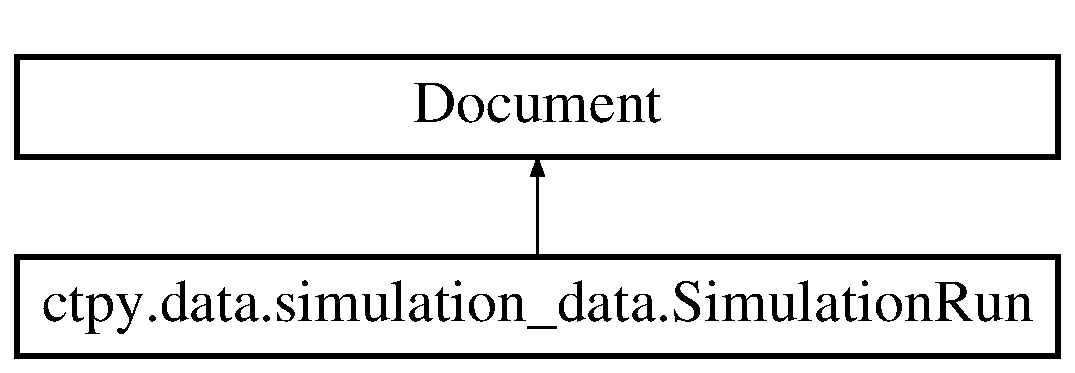
\includegraphics[height=2.000000cm]{classctpy_1_1data_1_1simulation__data_1_1_simulation_run}
\end{center}
\end{figure}
\subsection*{Classes}
\begin{DoxyCompactItemize}
\item 
class \hyperlink{classctpy_1_1data_1_1simulation__data_1_1_simulation_run_1_1____mongometa____}{\-\_\-\-\_\-mongometa\-\_\-\-\_\-}
\end{DoxyCompactItemize}
\subsection*{Static Public Attributes}
\begin{DoxyCompactItemize}
\item 
\hypertarget{classctpy_1_1data_1_1simulation__data_1_1_simulation_run_a4df73742b082e2fa5b7572766e23e8a8}{tuple {\bfseries script\-\_\-filename} = Field(str)}\label{classctpy_1_1data_1_1simulation__data_1_1_simulation_run_a4df73742b082e2fa5b7572766e23e8a8}

\item 
\hypertarget{classctpy_1_1data_1_1simulation__data_1_1_simulation_run_aa8837aff2316d00ac885d89fc71f9d76}{tuple {\bfseries replicates} = Field(int)}\label{classctpy_1_1data_1_1simulation__data_1_1_simulation_run_aa8837aff2316d00ac885d89fc71f9d76}

\item 
\hypertarget{classctpy_1_1data_1_1simulation__data_1_1_simulation_run_a125bb01518bd687c61fe8a556c8a8c30}{tuple {\bfseries num\-\_\-loci} = Field(int)}\label{classctpy_1_1data_1_1simulation__data_1_1_simulation_run_a125bb01518bd687c61fe8a556c8a8c30}

\item 
\hypertarget{classctpy_1_1data_1_1simulation__data_1_1_simulation_run_ad8a7fc40dc6eb1d351f6c64528c04792}{tuple {\bfseries sample\-\_\-size} = Field(int)}\label{classctpy_1_1data_1_1simulation__data_1_1_simulation_run_ad8a7fc40dc6eb1d351f6c64528c04792}

\item 
\hypertarget{classctpy_1_1data_1_1simulation__data_1_1_simulation_run_a36e06750c2922f4600d440bf203bb430}{tuple {\bfseries population\-\_\-size} = Field(int)}\label{classctpy_1_1data_1_1simulation__data_1_1_simulation_run_a36e06750c2922f4600d440bf203bb430}

\item 
\hypertarget{classctpy_1_1data_1_1simulation__data_1_1_simulation_run_a84870ab9688ce7cb3067fa6e438c872d}{tuple {\bfseries mutation\-\_\-rate} = Field(float)}\label{classctpy_1_1data_1_1simulation__data_1_1_simulation_run_a84870ab9688ce7cb3067fa6e438c872d}

\item 
\hypertarget{classctpy_1_1data_1_1simulation__data_1_1_simulation_run_aa4b992e3463e8598aa510203b1756b66}{tuple {\bfseries simulation\-\_\-run\-\_\-id} = Field(str)}\label{classctpy_1_1data_1_1simulation__data_1_1_simulation_run_aa4b992e3463e8598aa510203b1756b66}

\item 
\hypertarget{classctpy_1_1data_1_1simulation__data_1_1_simulation_run_a8c0a7043a1b310f2a49caff66a543f5f}{tuple {\bfseries num\-\_\-initial\-\_\-alleles} = Field(int)}\label{classctpy_1_1data_1_1simulation__data_1_1_simulation_run_a8c0a7043a1b310f2a49caff66a543f5f}

\item 
\hypertarget{classctpy_1_1data_1_1simulation__data_1_1_simulation_run_a6d3b9e680dcdbf92fdf89a43fc3656a5}{tuple {\bfseries max\-\_\-alleles} = Field(int)}\label{classctpy_1_1data_1_1simulation__data_1_1_simulation_run_a6d3b9e680dcdbf92fdf89a43fc3656a5}

\end{DoxyCompactItemize}


The documentation for this class was generated from the following file\-:\begin{DoxyCompactItemize}
\item 
ctpy/data/simulation\-\_\-data.\-py\end{DoxyCompactItemize}

\hypertarget{classtest__innovation__interval__stats_1_1_test_innovation_interval_stats}{\section{test\-\_\-innovation\-\_\-interval\-\_\-stats.\-Test\-Innovation\-Interval\-Stats Class Reference}
\label{classtest__innovation__interval__stats_1_1_test_innovation_interval_stats}\index{test\-\_\-innovation\-\_\-interval\-\_\-stats.\-Test\-Innovation\-Interval\-Stats@{test\-\_\-innovation\-\_\-interval\-\_\-stats.\-Test\-Innovation\-Interval\-Stats}}
}
Inheritance diagram for test\-\_\-innovation\-\_\-interval\-\_\-stats.\-Test\-Innovation\-Interval\-Stats\-:\begin{figure}[H]
\begin{center}
\leavevmode
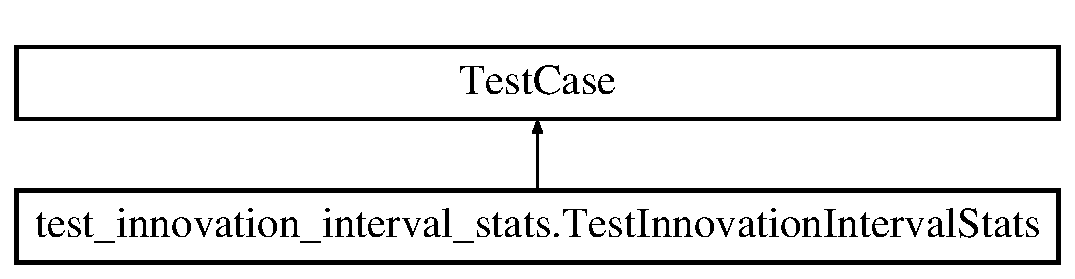
\includegraphics[height=2.000000cm]{classtest__innovation__interval__stats_1_1_test_innovation_interval_stats}
\end{center}
\end{figure}
\subsection*{Public Member Functions}
\begin{DoxyCompactItemize}
\item 
\hypertarget{classtest__innovation__interval__stats_1_1_test_innovation_interval_stats_a5c9d017a45cff00b45cf054185319b31}{def {\bfseries set\-Up}}\label{classtest__innovation__interval__stats_1_1_test_innovation_interval_stats_a5c9d017a45cff00b45cf054185319b31}

\item 
\hypertarget{classtest__innovation__interval__stats_1_1_test_innovation_interval_stats_a062f28a063d38a3c09c766a8d521ba34}{def {\bfseries test\-\_\-mean}}\label{classtest__innovation__interval__stats_1_1_test_innovation_interval_stats_a062f28a063d38a3c09c766a8d521ba34}

\item 
\hypertarget{classtest__innovation__interval__stats_1_1_test_innovation_interval_stats_aab3abfbea9309ab0240584c3b5df776c}{def {\bfseries test\-\_\-sd}}\label{classtest__innovation__interval__stats_1_1_test_innovation_interval_stats_aab3abfbea9309ab0240584c3b5df776c}

\end{DoxyCompactItemize}
\subsection*{Public Attributes}
\begin{DoxyCompactItemize}
\item 
\hypertarget{classtest__innovation__interval__stats_1_1_test_innovation_interval_stats_a4a02d72123db0217f66244540777805b}{{\bfseries config}}\label{classtest__innovation__interval__stats_1_1_test_innovation_interval_stats_a4a02d72123db0217f66244540777805b}

\item 
\hypertarget{classtest__innovation__interval__stats_1_1_test_innovation_interval_stats_a6c85d479879f3caeb308140b29a46e56}{{\bfseries test\-\_\-data}}\label{classtest__innovation__interval__stats_1_1_test_innovation_interval_stats_a6c85d479879f3caeb308140b29a46e56}

\item 
\hypertarget{classtest__innovation__interval__stats_1_1_test_innovation_interval_stats_a3126a3c7529aa52fd9de11611500a135}{{\bfseries expected\-\_\-intervals}}\label{classtest__innovation__interval__stats_1_1_test_innovation_interval_stats_a3126a3c7529aa52fd9de11611500a135}

\item 
\hypertarget{classtest__innovation__interval__stats_1_1_test_innovation_interval_stats_ac021fdf20ed2e03d3b62164c03af4703}{{\bfseries expected\-\_\-mean\-\_\-interval}}\label{classtest__innovation__interval__stats_1_1_test_innovation_interval_stats_ac021fdf20ed2e03d3b62164c03af4703}

\item 
\hypertarget{classtest__innovation__interval__stats_1_1_test_innovation_interval_stats_a690f564f03acb1ff2ba365d1fe68b75b}{{\bfseries expected\-\_\-sd\-\_\-interval}}\label{classtest__innovation__interval__stats_1_1_test_innovation_interval_stats_a690f564f03acb1ff2ba365d1fe68b75b}

\item 
\hypertarget{classtest__innovation__interval__stats_1_1_test_innovation_interval_stats_aead65a35b917b82d15e8a69abd331b88}{{\bfseries epsilon}}\label{classtest__innovation__interval__stats_1_1_test_innovation_interval_stats_aead65a35b917b82d15e8a69abd331b88}

\item 
\hypertarget{classtest__innovation__interval__stats_1_1_test_innovation_interval_stats_a970fb641bfb8dcd3b394cd0ace0a92e7}{{\bfseries stats}}\label{classtest__innovation__interval__stats_1_1_test_innovation_interval_stats_a970fb641bfb8dcd3b394cd0ace0a92e7}

\end{DoxyCompactItemize}


The documentation for this class was generated from the following file\-:\begin{DoxyCompactItemize}
\item 
test/test\-\_\-innovation\-\_\-interval\-\_\-stats.\-py\end{DoxyCompactItemize}

\hypertarget{classtest__update__data_1_1_test_update_data}{\section{test\-\_\-update\-\_\-data.\-Test\-Update\-Data Class Reference}
\label{classtest__update__data_1_1_test_update_data}\index{test\-\_\-update\-\_\-data.\-Test\-Update\-Data@{test\-\_\-update\-\_\-data.\-Test\-Update\-Data}}
}
Inheritance diagram for test\-\_\-update\-\_\-data.\-Test\-Update\-Data\-:\begin{figure}[H]
\begin{center}
\leavevmode
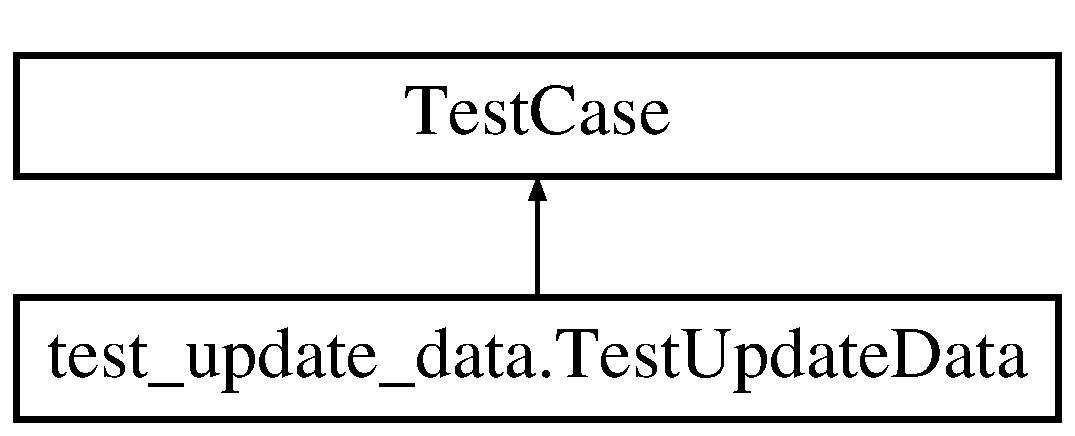
\includegraphics[height=2.000000cm]{classtest__update__data_1_1_test_update_data}
\end{center}
\end{figure}
\subsection*{Public Member Functions}
\begin{DoxyCompactItemize}
\item 
\hypertarget{classtest__update__data_1_1_test_update_data_a4c3c4d45fdcdce4fb85c64b024617bf6}{def {\bfseries set\-Up}}\label{classtest__update__data_1_1_test_update_data_a4c3c4d45fdcdce4fb85c64b024617bf6}

\item 
\hypertarget{classtest__update__data_1_1_test_update_data_aed110b33125f51888a168e265b8d72e9}{def {\bfseries test\-\_\-update}}\label{classtest__update__data_1_1_test_update_data_aed110b33125f51888a168e265b8d72e9}

\end{DoxyCompactItemize}
\subsection*{Public Attributes}
\begin{DoxyCompactItemize}
\item 
\hypertarget{classtest__update__data_1_1_test_update_data_a4902d5786ceeaded3ee22d4c5ffce6cc}{{\bfseries data}}\label{classtest__update__data_1_1_test_update_data_a4902d5786ceeaded3ee22d4c5ffce6cc}

\end{DoxyCompactItemize}


The documentation for this class was generated from the following file\-:\begin{DoxyCompactItemize}
\item 
test/test\-\_\-update\-\_\-data.\-py\end{DoxyCompactItemize}

\hypertarget{classctpy_1_1data_1_1trait__count__population_1_1_trait_count_sample}{\section{ctpy.\-data.\-trait\-\_\-count\-\_\-population.\-Trait\-Count\-Sample Class Reference}
\label{classctpy_1_1data_1_1trait__count__population_1_1_trait_count_sample}\index{ctpy.\-data.\-trait\-\_\-count\-\_\-population.\-Trait\-Count\-Sample@{ctpy.\-data.\-trait\-\_\-count\-\_\-population.\-Trait\-Count\-Sample}}
}
Inheritance diagram for ctpy.\-data.\-trait\-\_\-count\-\_\-population.\-Trait\-Count\-Sample\-:\begin{figure}[H]
\begin{center}
\leavevmode
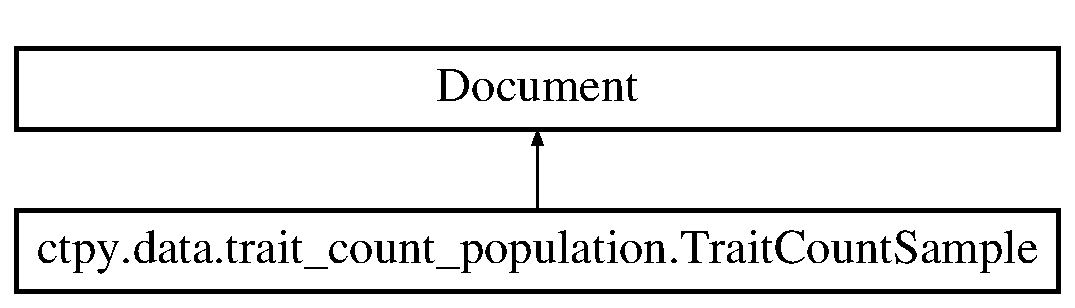
\includegraphics[height=2.000000cm]{classctpy_1_1data_1_1trait__count__population_1_1_trait_count_sample}
\end{center}
\end{figure}
\subsection*{Classes}
\begin{DoxyCompactItemize}
\item 
class \hyperlink{classctpy_1_1data_1_1trait__count__population_1_1_trait_count_sample_1_1____mongometa____}{\-\_\-\-\_\-mongometa\-\_\-\-\_\-}
\end{DoxyCompactItemize}
\subsection*{Static Public Attributes}
\begin{DoxyCompactItemize}
\item 
\hypertarget{classctpy_1_1data_1_1trait__count__population_1_1_trait_count_sample_a929e8abc40bbc300fdf3550b404392d0}{tuple {\bfseries simulation\-\_\-time} = Field(int)}\label{classctpy_1_1data_1_1trait__count__population_1_1_trait_count_sample_a929e8abc40bbc300fdf3550b404392d0}

\item 
\hypertarget{classctpy_1_1data_1_1trait__count__population_1_1_trait_count_sample_a153ac22e85aa8b7881dc6cd9bf695f81}{tuple {\bfseries replication} = Field(int)}\label{classctpy_1_1data_1_1trait__count__population_1_1_trait_count_sample_a153ac22e85aa8b7881dc6cd9bf695f81}

\item 
\hypertarget{classctpy_1_1data_1_1trait__count__population_1_1_trait_count_sample_aa6790e220da226ac39bffdf0f16e72a6}{tuple {\bfseries locus} = Field(int)}\label{classctpy_1_1data_1_1trait__count__population_1_1_trait_count_sample_aa6790e220da226ac39bffdf0f16e72a6}

\item 
\hypertarget{classctpy_1_1data_1_1trait__count__population_1_1_trait_count_sample_a8bef14ceca555d393710f4e6edb9cf7c}{tuple {\bfseries population\-\_\-size} = Field(int)}\label{classctpy_1_1data_1_1trait__count__population_1_1_trait_count_sample_a8bef14ceca555d393710f4e6edb9cf7c}

\item 
\hypertarget{classctpy_1_1data_1_1trait__count__population_1_1_trait_count_sample_ac3bbe96a5b5679c57b62ff4f825c80d3}{tuple {\bfseries mutation\-\_\-rate} = Field(float)}\label{classctpy_1_1data_1_1trait__count__population_1_1_trait_count_sample_ac3bbe96a5b5679c57b62ff4f825c80d3}

\item 
\hypertarget{classctpy_1_1data_1_1trait__count__population_1_1_trait_count_sample_aeb4a48abd2ff007caf8129eed8a7a74a}{tuple {\bfseries simulation\-\_\-run\-\_\-id} = Field(str)}\label{classctpy_1_1data_1_1trait__count__population_1_1_trait_count_sample_aeb4a48abd2ff007caf8129eed8a7a74a}

\item 
\hypertarget{classctpy_1_1data_1_1trait__count__population_1_1_trait_count_sample_a7f4a791925eb3b6db848f59b52a91ba1}{tuple {\bfseries allele} = Field(int)}\label{classctpy_1_1data_1_1trait__count__population_1_1_trait_count_sample_a7f4a791925eb3b6db848f59b52a91ba1}

\item 
\hypertarget{classctpy_1_1data_1_1trait__count__population_1_1_trait_count_sample_aa92a605257c9adb668bcbc48337a4ea0}{tuple {\bfseries count} = Field(float)}\label{classctpy_1_1data_1_1trait__count__population_1_1_trait_count_sample_aa92a605257c9adb668bcbc48337a4ea0}

\end{DoxyCompactItemize}


The documentation for this class was generated from the following file\-:\begin{DoxyCompactItemize}
\item 
ctpy/data/trait\-\_\-count\-\_\-population.\-py\end{DoxyCompactItemize}

\hypertarget{classctpy_1_1data_1_1trait__count__sample_1_1_trait_count_sample}{\section{ctpy.\-data.\-trait\-\_\-count\-\_\-sample.\-Trait\-Count\-Sample Class Reference}
\label{classctpy_1_1data_1_1trait__count__sample_1_1_trait_count_sample}\index{ctpy.\-data.\-trait\-\_\-count\-\_\-sample.\-Trait\-Count\-Sample@{ctpy.\-data.\-trait\-\_\-count\-\_\-sample.\-Trait\-Count\-Sample}}
}
Inheritance diagram for ctpy.\-data.\-trait\-\_\-count\-\_\-sample.\-Trait\-Count\-Sample\-:\begin{figure}[H]
\begin{center}
\leavevmode
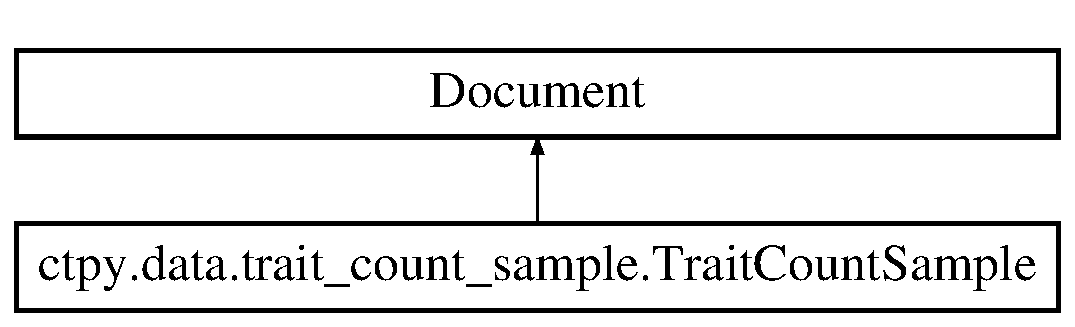
\includegraphics[height=2.000000cm]{classctpy_1_1data_1_1trait__count__sample_1_1_trait_count_sample}
\end{center}
\end{figure}
\subsection*{Classes}
\begin{DoxyCompactItemize}
\item 
class \hyperlink{classctpy_1_1data_1_1trait__count__sample_1_1_trait_count_sample_1_1____mongometa____}{\-\_\-\-\_\-mongometa\-\_\-\-\_\-}
\end{DoxyCompactItemize}
\subsection*{Static Public Attributes}
\begin{DoxyCompactItemize}
\item 
\hypertarget{classctpy_1_1data_1_1trait__count__sample_1_1_trait_count_sample_aa89ff4003d4ad212a0a2044bfbc8272b}{tuple {\bfseries simulation\-\_\-time} = Field(int)}\label{classctpy_1_1data_1_1trait__count__sample_1_1_trait_count_sample_aa89ff4003d4ad212a0a2044bfbc8272b}

\item 
\hypertarget{classctpy_1_1data_1_1trait__count__sample_1_1_trait_count_sample_adbe43cbab49af898bf28fb23f4bd0619}{tuple {\bfseries replication} = Field(int)}\label{classctpy_1_1data_1_1trait__count__sample_1_1_trait_count_sample_adbe43cbab49af898bf28fb23f4bd0619}

\item 
\hypertarget{classctpy_1_1data_1_1trait__count__sample_1_1_trait_count_sample_a3908478d3d7da0c280c2b1ef8dd07f34}{tuple {\bfseries locus} = Field(int)}\label{classctpy_1_1data_1_1trait__count__sample_1_1_trait_count_sample_a3908478d3d7da0c280c2b1ef8dd07f34}

\item 
\hypertarget{classctpy_1_1data_1_1trait__count__sample_1_1_trait_count_sample_a87443b775ba76c688a912d3f56627126}{tuple {\bfseries sample\-\_\-size} = Field(int)}\label{classctpy_1_1data_1_1trait__count__sample_1_1_trait_count_sample_a87443b775ba76c688a912d3f56627126}

\item 
\hypertarget{classctpy_1_1data_1_1trait__count__sample_1_1_trait_count_sample_a1bcfc1500a05fa001e4d4d8ac7bfe7b8}{tuple {\bfseries population\-\_\-size} = Field(int)}\label{classctpy_1_1data_1_1trait__count__sample_1_1_trait_count_sample_a1bcfc1500a05fa001e4d4d8ac7bfe7b8}

\item 
\hypertarget{classctpy_1_1data_1_1trait__count__sample_1_1_trait_count_sample_a318b84cb171b9f16652f99d33b47cd96}{tuple {\bfseries mutation\-\_\-rate} = Field(float)}\label{classctpy_1_1data_1_1trait__count__sample_1_1_trait_count_sample_a318b84cb171b9f16652f99d33b47cd96}

\item 
\hypertarget{classctpy_1_1data_1_1trait__count__sample_1_1_trait_count_sample_a53d4455d16b87408a329edab30b25e48}{tuple {\bfseries simulation\-\_\-run\-\_\-id} = Field(str)}\label{classctpy_1_1data_1_1trait__count__sample_1_1_trait_count_sample_a53d4455d16b87408a329edab30b25e48}

\item 
\hypertarget{classctpy_1_1data_1_1trait__count__sample_1_1_trait_count_sample_a4302dc23e3709cd5c42d90a1ce015bee}{tuple {\bfseries allele} = Field(int)}\label{classctpy_1_1data_1_1trait__count__sample_1_1_trait_count_sample_a4302dc23e3709cd5c42d90a1ce015bee}

\item 
\hypertarget{classctpy_1_1data_1_1trait__count__sample_1_1_trait_count_sample_a63f3169f758c96b45199a72bdf2737d5}{tuple {\bfseries count} = Field(float)}\label{classctpy_1_1data_1_1trait__count__sample_1_1_trait_count_sample_a63f3169f758c96b45199a72bdf2737d5}

\end{DoxyCompactItemize}


The documentation for this class was generated from the following file\-:\begin{DoxyCompactItemize}
\item 
ctpy/data/trait\-\_\-count\-\_\-sample.\-py\end{DoxyCompactItemize}

\hypertarget{classctpy_1_1data_1_1trait__lifetime_1_1_trait_lifetime_cache_i_a_models}{\section{ctpy.\-data.\-trait\-\_\-lifetime.\-Trait\-Lifetime\-Cache\-I\-A\-Models Class Reference}
\label{classctpy_1_1data_1_1trait__lifetime_1_1_trait_lifetime_cache_i_a_models}\index{ctpy.\-data.\-trait\-\_\-lifetime.\-Trait\-Lifetime\-Cache\-I\-A\-Models@{ctpy.\-data.\-trait\-\_\-lifetime.\-Trait\-Lifetime\-Cache\-I\-A\-Models}}
}


Caches the starting generation of each newly mutated allele.  


\subsection*{Public Member Functions}
\begin{DoxyCompactItemize}
\item 
\hypertarget{classctpy_1_1data_1_1trait__lifetime_1_1_trait_lifetime_cache_i_a_models_aa8f37e27c5e6c87657232372b748c6ba}{def {\bfseries \-\_\-\-\_\-init\-\_\-\-\_\-}}\label{classctpy_1_1data_1_1trait__lifetime_1_1_trait_lifetime_cache_i_a_models_aa8f37e27c5e6c87657232372b748c6ba}

\item 
\hypertarget{classctpy_1_1data_1_1trait__lifetime_1_1_trait_lifetime_cache_i_a_models_ae8808c305c0c7bd0c9a95aa5bcc15d29}{def {\bfseries debug\-Print\-Origin\-Cache}}\label{classctpy_1_1data_1_1trait__lifetime_1_1_trait_lifetime_cache_i_a_models_ae8808c305c0c7bd0c9a95aa5bcc15d29}

\item 
\hypertarget{classctpy_1_1data_1_1trait__lifetime_1_1_trait_lifetime_cache_i_a_models_a79dd58583fc674ec882f7e8119c563b0}{def \hyperlink{classctpy_1_1data_1_1trait__lifetime_1_1_trait_lifetime_cache_i_a_models_a79dd58583fc674ec882f7e8119c563b0}{allele\-\_\-origin\-\_\-tracker}}\label{classctpy_1_1data_1_1trait__lifetime_1_1_trait_lifetime_cache_i_a_models_a79dd58583fc674ec882f7e8119c563b0}

\begin{DoxyCompactList}\small\item\em Used as an output function in a simu\-P\-O\-P mutator, post 1.\-11. \end{DoxyCompactList}\item 
def \hyperlink{classctpy_1_1data_1_1trait__lifetime_1_1_trait_lifetime_cache_i_a_models_ab75d75f7c965b390dadc6a210cc860eb}{allele\-\_\-demise\-\_\-tracker}
\begin{DoxyCompactList}\small\item\em Checks to see if any traits have gone to zero frequency and thus exited the population. \end{DoxyCompactList}\end{DoxyCompactItemize}
\subsection*{Public Attributes}
\begin{DoxyCompactItemize}
\item 
\hypertarget{classctpy_1_1data_1_1trait__lifetime_1_1_trait_lifetime_cache_i_a_models_a97d755b0300aad41ae2afb6447cf89af}{{\bfseries origin\-\_\-cache}}\label{classctpy_1_1data_1_1trait__lifetime_1_1_trait_lifetime_cache_i_a_models_a97d755b0300aad41ae2afb6447cf89af}

\end{DoxyCompactItemize}


\subsection{Detailed Description}
Caches the starting generation of each newly mutated allele. 

Constructor takes as argument the number of loci and initial alleles, since these begin their lifetime at gen 0.

N\-O\-T\-E\-: This class is appropriate O\-N\-L\-Y for infinite alleles models, with no back-\/mutation or other mechanisms by which a trait can \char`\"{}come back\char`\"{} from an exit. 

\subsection{Member Function Documentation}
\hypertarget{classctpy_1_1data_1_1trait__lifetime_1_1_trait_lifetime_cache_i_a_models_ab75d75f7c965b390dadc6a210cc860eb}{\index{ctpy\-::data\-::trait\-\_\-lifetime\-::\-Trait\-Lifetime\-Cache\-I\-A\-Models@{ctpy\-::data\-::trait\-\_\-lifetime\-::\-Trait\-Lifetime\-Cache\-I\-A\-Models}!allele\-\_\-demise\-\_\-tracker@{allele\-\_\-demise\-\_\-tracker}}
\index{allele\-\_\-demise\-\_\-tracker@{allele\-\_\-demise\-\_\-tracker}!ctpy::data::trait_lifetime::TraitLifetimeCacheIAModels@{ctpy\-::data\-::trait\-\_\-lifetime\-::\-Trait\-Lifetime\-Cache\-I\-A\-Models}}
\subsubsection[{allele\-\_\-demise\-\_\-tracker}]{\setlength{\rightskip}{0pt plus 5cm}def ctpy.\-data.\-trait\-\_\-lifetime.\-Trait\-Lifetime\-Cache\-I\-A\-Models.\-allele\-\_\-demise\-\_\-tracker (
\begin{DoxyParamCaption}
\item[{}]{self, }
\item[{}]{pop, }
\item[{}]{param}
\end{DoxyParamCaption}
)}}\label{classctpy_1_1data_1_1trait__lifetime_1_1_trait_lifetime_cache_i_a_models_ab75d75f7c965b390dadc6a210cc860eb}


Checks to see if any traits have gone to zero frequency and thus exited the population. 

If a trait has exited, the generation of exit is recorded in the cache, and a record inserted into the database recording the total lifetime in generations of the trait.

N\-O\-T\-E\-: This operator is appropriate O\-N\-L\-Y for infinite alleles models, with no back-\/mutation or other mechanisms by which a trait can \char`\"{}come back\char`\"{} from an exit.

Args\-: \begin{DoxyVerb}pop (Population):  simuPOP population replicate.

params (list):  list of parameters (sample size, mutation rate, population size, simulation ID, number of loci)
\end{DoxyVerb}


Returns\-: \begin{DoxyVerb}Boolean true:  all PyOperators need to return true\end{DoxyVerb}
 

The documentation for this class was generated from the following file\-:\begin{DoxyCompactItemize}
\item 
ctpy/data/trait\-\_\-lifetime.\-py\end{DoxyCompactItemize}

\hypertarget{classctpy_1_1data_1_1trait__lifetime_1_1_trait_lifetime_record}{\section{ctpy.\-data.\-trait\-\_\-lifetime.\-Trait\-Lifetime\-Record Class Reference}
\label{classctpy_1_1data_1_1trait__lifetime_1_1_trait_lifetime_record}\index{ctpy.\-data.\-trait\-\_\-lifetime.\-Trait\-Lifetime\-Record@{ctpy.\-data.\-trait\-\_\-lifetime.\-Trait\-Lifetime\-Record}}
}
Inheritance diagram for ctpy.\-data.\-trait\-\_\-lifetime.\-Trait\-Lifetime\-Record\-:\begin{figure}[H]
\begin{center}
\leavevmode
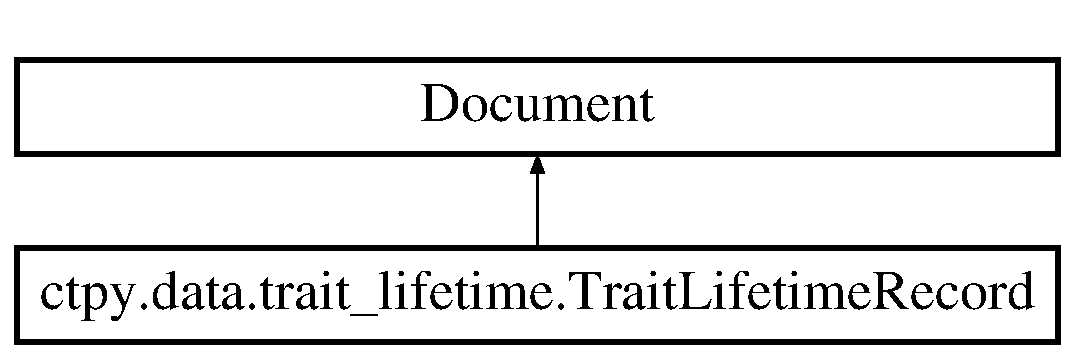
\includegraphics[height=2.000000cm]{classctpy_1_1data_1_1trait__lifetime_1_1_trait_lifetime_record}
\end{center}
\end{figure}
\subsection*{Classes}
\begin{DoxyCompactItemize}
\item 
class \hyperlink{classctpy_1_1data_1_1trait__lifetime_1_1_trait_lifetime_record_1_1____mongometa____}{\-\_\-\-\_\-mongometa\-\_\-\-\_\-}
\end{DoxyCompactItemize}
\subsection*{Static Public Attributes}
\begin{DoxyCompactItemize}
\item 
\hypertarget{classctpy_1_1data_1_1trait__lifetime_1_1_trait_lifetime_record_a34329c77033b3422941b5034210c8ec6}{tuple {\bfseries replication} = Field(int)}\label{classctpy_1_1data_1_1trait__lifetime_1_1_trait_lifetime_record_a34329c77033b3422941b5034210c8ec6}

\item 
\hypertarget{classctpy_1_1data_1_1trait__lifetime_1_1_trait_lifetime_record_abfcbbed46d42754bb88ab176fc271b19}{tuple {\bfseries locus} = Field(int)}\label{classctpy_1_1data_1_1trait__lifetime_1_1_trait_lifetime_record_abfcbbed46d42754bb88ab176fc271b19}

\item 
\hypertarget{classctpy_1_1data_1_1trait__lifetime_1_1_trait_lifetime_record_ab0cd686096450ceb9a9d5333b873cb8a}{tuple {\bfseries population\-\_\-size} = Field(int)}\label{classctpy_1_1data_1_1trait__lifetime_1_1_trait_lifetime_record_ab0cd686096450ceb9a9d5333b873cb8a}

\item 
\hypertarget{classctpy_1_1data_1_1trait__lifetime_1_1_trait_lifetime_record_ae2d69a03e8375928d093599c8752cd95}{tuple {\bfseries sample\-\_\-size} = Field(int)}\label{classctpy_1_1data_1_1trait__lifetime_1_1_trait_lifetime_record_ae2d69a03e8375928d093599c8752cd95}

\item 
\hypertarget{classctpy_1_1data_1_1trait__lifetime_1_1_trait_lifetime_record_a4d1b3124976e2428d1966cfe5cb30f26}{tuple {\bfseries mutation\-\_\-rate} = Field(float)}\label{classctpy_1_1data_1_1trait__lifetime_1_1_trait_lifetime_record_a4d1b3124976e2428d1966cfe5cb30f26}

\item 
\hypertarget{classctpy_1_1data_1_1trait__lifetime_1_1_trait_lifetime_record_a45be5dd9ab144209a493c552b5e2fcf3}{tuple {\bfseries simulation\-\_\-run\-\_\-id} = Field(str)}\label{classctpy_1_1data_1_1trait__lifetime_1_1_trait_lifetime_record_a45be5dd9ab144209a493c552b5e2fcf3}

\item 
\hypertarget{classctpy_1_1data_1_1trait__lifetime_1_1_trait_lifetime_record_aaec42f993041c174518023637ee97bc0}{tuple {\bfseries allele} = Field(int)}\label{classctpy_1_1data_1_1trait__lifetime_1_1_trait_lifetime_record_aaec42f993041c174518023637ee97bc0}

\item 
\hypertarget{classctpy_1_1data_1_1trait__lifetime_1_1_trait_lifetime_record_aa02fc335d053c6e90e2785eb837daf22}{tuple {\bfseries lifetime} = Field(int)}\label{classctpy_1_1data_1_1trait__lifetime_1_1_trait_lifetime_record_aa02fc335d053c6e90e2785eb837daf22}

\end{DoxyCompactItemize}


The documentation for this class was generated from the following file\-:\begin{DoxyCompactItemize}
\item 
ctpy/data/trait\-\_\-lifetime.\-py\end{DoxyCompactItemize}

\hypertarget{classctpy_1_1math_1_1trait__statistics_1_1_trait_statistics_per_sample}{\section{ctpy.\-math.\-trait\-\_\-statistics.\-Trait\-Statistics\-Per\-Sample Class Reference}
\label{classctpy_1_1math_1_1trait__statistics_1_1_trait_statistics_per_sample}\index{ctpy.\-math.\-trait\-\_\-statistics.\-Trait\-Statistics\-Per\-Sample@{ctpy.\-math.\-trait\-\_\-statistics.\-Trait\-Statistics\-Per\-Sample}}
}
\subsection*{Public Member Functions}
\begin{DoxyCompactItemize}
\item 
\hypertarget{classctpy_1_1math_1_1trait__statistics_1_1_trait_statistics_per_sample_ab11ed10d974dd4f2873ef6a283ed30ab}{def {\bfseries \-\_\-\-\_\-init\-\_\-\-\_\-}}\label{classctpy_1_1math_1_1trait__statistics_1_1_trait_statistics_per_sample_ab11ed10d974dd4f2873ef6a283ed30ab}

\item 
def \hyperlink{classctpy_1_1math_1_1trait__statistics_1_1_trait_statistics_per_sample_a368e901d667a703f72ef4b6aff9738b5}{process\-\_\-trait\-\_\-statistics}
\begin{DoxyCompactList}\small\item\em Given a sample in the fulldataset, we want to calculate the following\-: trait richness per locus for sample, mean trait richness per generation for sample, shannon entropy and iqv per locus for sample, mean shannon entropy and iqv per generation for sample. \end{DoxyCompactList}\item 
def \hyperlink{classctpy_1_1math_1_1trait__statistics_1_1_trait_statistics_per_sample_a6c5bd126d94e0b27407d70fd5fc035a6}{update\-\_\-with\-\_\-slatkin\-\_\-test}
\begin{DoxyCompactList}\small\item\em Given a per generation trait statistics record, we get the original sample, total its trait counts, get the slatkin exact neutrality result, and U\-P\-D\-A\-T\-E the per generation trait statistics record. \end{DoxyCompactList}\end{DoxyCompactItemize}
\subsection*{Public Attributes}
\begin{DoxyCompactItemize}
\item 
\hypertarget{classctpy_1_1math_1_1trait__statistics_1_1_trait_statistics_per_sample_a1e19ba5922fcdaf9a80d3633dad30f36}{{\bfseries simconfig}}\label{classctpy_1_1math_1_1trait__statistics_1_1_trait_statistics_per_sample_a1e19ba5922fcdaf9a80d3633dad30f36}

\item 
\hypertarget{classctpy_1_1math_1_1trait__statistics_1_1_trait_statistics_per_sample_a64dd95776aefda9aa63d255b20f1a660}{{\bfseries sample}}\label{classctpy_1_1math_1_1trait__statistics_1_1_trait_statistics_per_sample_a64dd95776aefda9aa63d255b20f1a660}

\end{DoxyCompactItemize}


\subsection{Member Function Documentation}
\hypertarget{classctpy_1_1math_1_1trait__statistics_1_1_trait_statistics_per_sample_a368e901d667a703f72ef4b6aff9738b5}{\index{ctpy\-::math\-::trait\-\_\-statistics\-::\-Trait\-Statistics\-Per\-Sample@{ctpy\-::math\-::trait\-\_\-statistics\-::\-Trait\-Statistics\-Per\-Sample}!process\-\_\-trait\-\_\-statistics@{process\-\_\-trait\-\_\-statistics}}
\index{process\-\_\-trait\-\_\-statistics@{process\-\_\-trait\-\_\-statistics}!ctpy::math::trait_statistics::TraitStatisticsPerSample@{ctpy\-::math\-::trait\-\_\-statistics\-::\-Trait\-Statistics\-Per\-Sample}}
\subsubsection[{process\-\_\-trait\-\_\-statistics}]{\setlength{\rightskip}{0pt plus 5cm}def ctpy.\-math.\-trait\-\_\-statistics.\-Trait\-Statistics\-Per\-Sample.\-process\-\_\-trait\-\_\-statistics (
\begin{DoxyParamCaption}
\item[{}]{self}
\end{DoxyParamCaption}
)}}\label{classctpy_1_1math_1_1trait__statistics_1_1_trait_statistics_per_sample_a368e901d667a703f72ef4b6aff9738b5}


Given a sample in the fulldataset, we want to calculate the following\-: trait richness per locus for sample, mean trait richness per generation for sample, shannon entropy and iqv per locus for sample, mean shannon entropy and iqv per generation for sample. 

These statistics are saved to the database with sim run I\-D, replication, sample size, mutation rate, simulation time, and population size as keys. With these keys, we can match them up to their post-\/classification counterparts.

\-:return\-: no return value \hypertarget{classctpy_1_1math_1_1trait__statistics_1_1_trait_statistics_per_sample_a6c5bd126d94e0b27407d70fd5fc035a6}{\index{ctpy\-::math\-::trait\-\_\-statistics\-::\-Trait\-Statistics\-Per\-Sample@{ctpy\-::math\-::trait\-\_\-statistics\-::\-Trait\-Statistics\-Per\-Sample}!update\-\_\-with\-\_\-slatkin\-\_\-test@{update\-\_\-with\-\_\-slatkin\-\_\-test}}
\index{update\-\_\-with\-\_\-slatkin\-\_\-test@{update\-\_\-with\-\_\-slatkin\-\_\-test}!ctpy::math::trait_statistics::TraitStatisticsPerSample@{ctpy\-::math\-::trait\-\_\-statistics\-::\-Trait\-Statistics\-Per\-Sample}}
\subsubsection[{update\-\_\-with\-\_\-slatkin\-\_\-test}]{\setlength{\rightskip}{0pt plus 5cm}def ctpy.\-math.\-trait\-\_\-statistics.\-Trait\-Statistics\-Per\-Sample.\-update\-\_\-with\-\_\-slatkin\-\_\-test (
\begin{DoxyParamCaption}
\item[{}]{self}
\end{DoxyParamCaption}
)}}\label{classctpy_1_1math_1_1trait__statistics_1_1_trait_statistics_per_sample_a6c5bd126d94e0b27407d70fd5fc035a6}


Given a per generation trait statistics record, we get the original sample, total its trait counts, get the slatkin exact neutrality result, and U\-P\-D\-A\-T\-E the per generation trait statistics record. 

\-:return\-: 

The documentation for this class was generated from the following file\-:\begin{DoxyCompactItemize}
\item 
ctpy/math/trait\-\_\-statistics.\-py\end{DoxyCompactItemize}

%--- End generated contents ---

% Index
\newpage
\phantomsection
\addcontentsline{toc}{part}{Index}
\printindex

\end{document}
